% !TeX program = pdflatex
% !TeX root = proyecto.tex
\documentclass[a4paper,11pt]{book}
%\documentclass[a4paper,twoside,11pt,titlepage]{book}
\usepackage{listings}
\usepackage[utf8]{inputenc}
\usepackage[spanish]{babel}

% \usepackage[style=list, number=none]{glossary} %
%\usepackage{titlesec}
%\usepackage{pailatino}

\decimalpoint
\usepackage{dcolumn}
\newcolumntype{.}{D{.}{\esperiod}{-1}}
\makeatletter
\addto\shorthandsspanish{\let\esperiod\es@period@code}
\makeatother


%\usepackage[chapter]{algorithm}
\RequirePackage{verbatim}
%\RequirePackage[Glenn]{fncychap}
\usepackage{fancyhdr}
\usepackage{graphicx}
\usepackage{float}
\usepackage{afterpage}

\usepackage{longtable}

\usepackage{hyperref} %referencia

\usepackage[
backend=biber,
style=apa,
sorting=nyt
]{biblatex}

\DeclareLanguageMapping{spanish}{spanish-apa}

\addbibresource{bibliografia/referencias.bib}

% ********************************************************************
% Re-usable information
% ********************************************************************
\newcommand{\myTitle}{Sistema de medida del consumo energético de las CPU de un clúster de computadores}
\newcommand{\myDegree}{Grado en Ingeniería Informática}
\newcommand{\myName}{Alejandro Madueño Buciegas}
\newcommand{\myProf}{Jesús González Peñalver}
\newcommand{\myOtherProf}{Beatriz Prieto Campos}
%\newcommand{\mySupervisor}{Put name here\xspace}
\newcommand{\myFaculty}{Escuela Técnica Superior de Ingenierías Informática y de
Telecomunicación}
\newcommand{\myFacultyShort}{E.T.S. de Ingenierías Informática y de
Telecomunicación}
\newcommand{\myUni}{\protect{Universidad de Granada}}
\newcommand{\myLocation}{Granada}
\newcommand{\myTime}{\today}
\newcommand{\myVersion}{Versión final}


\hypersetup{
pdfauthor = {\myName},
pdftitle = {\myTitle},
pdfsubject = {Trabajo Fin de Grado sobre medida energética de CPU en un clúster},
pdfkeywords = {eficiencia energética, Intel RAPL, HPC, SLURM, monitorización},
pdfcreator = {LaTeX},
pdfproducer = {pdflatex},
colorlinks = true,
linkcolor = blue,
citecolor = blue,
urlcolor = blue,
}

%\hyphenation{}


%\usepackage{doxygen/doxygen}
%\usepackage{pdfpages}
\usepackage{url}
\usepackage{colortbl,longtable}

\setlength{\emergencystretch}{2em}
\setcounter{biburlnumpenalty}{100}
\setcounter{biburlucpenalty}{100}
\setcounter{biburllcpenalty}{100}

% Recuadro breve para destacar decisiones e incidencias de ingeniería.
\newcommand{\decisionbox}[2]{%
    \par\medskip
    \begin{center}
        \fcolorbox[gray]{0.35}{0.96}{%
            \begin{minipage}{0.90\textwidth}
                \small
                \textbf{#1}\par\smallskip
                #2
            \end{minipage}%
        }
    \end{center}
    \medskip
}

% Componentes vectoriales reutilizables para los esquemas de la memoria.
\newcommand{\diagramnode}[2][0.19\textwidth]{%
    \fcolorbox[gray]{0.35}{0.95}{%
        \parbox[c][1.85cm][c]{%
            \dimexpr#1-2\fboxsep-2\fboxrule\relax
        }{\centering\small #2}%
    }%
}
\newcommand{\diagramnodeaccent}[2][0.19\textwidth]{%
    \fcolorbox[gray]{0.25}{0.87}{%
        \parbox[c][1.85cm][c]{%
            \dimexpr#1-2\fboxsep-2\fboxrule\relax
        }{\centering\small\bfseries #2}%
    }%
}
\newcommand{\diagramarrow}{\hspace{0.10cm}\ensuremath{\longrightarrow}\hspace{0.10cm}}
\newcommand{\diagramleftarrow}{\hspace{0.10cm}\ensuremath{\longleftarrow}\hspace{0.10cm}}
\newcommand{\diagramdown}{\ensuremath{\Big\downarrow}}
\usepackage[stable]{footmisc}
%\usepackage{index}

%\makeindex
%\usepackage[style=long, cols=2,border=plain,toc=true,number=none]{glossary}
% \makeglossary

% Definición de comandos que me son tiles:
%\renewcommand{\indexname}{Índice alfabético}
%\renewcommand{\glossaryname}{Glosario}

\pagestyle{fancy}
\fancyhf{}
\fancyhead[LO]{\leftmark}
\fancyhead[RE]{\rightmark}
\fancyhead[RO,LE]{\textbf{\thepage}}
\renewcommand{\chaptermark}[1]{\markboth{\textbf{#1}}{}}
\renewcommand{\sectionmark}[1]{\markright{\textbf{\thesection. #1}}}

\setlength{\headheight}{1.5\headheight}

\newcommand{\HRule}{\rule{\linewidth}{0.5mm}}
%Definimos los tipos teorema, ejemplo y definición podremos usar estos tipos
%simplemente poniendo \begin{teorema} \end{teorema} ...
\newtheorem{teorema}{Teorema}[chapter]
\newtheorem{ejemplo}{Ejemplo}[chapter]
\newtheorem{definicion}{Definición}[chapter]

\definecolor{gray97}{gray}{.97}
\definecolor{gray75}{gray}{.75}
\definecolor{gray45}{gray}{.45}
\definecolor{gray30}{gray}{.94}

\lstset{ frame=Ltb,
     framerule=0.5pt,
     aboveskip=0.5cm,
     framextopmargin=3pt,
     framexbottommargin=3pt,
     framexleftmargin=0.1cm,
     framesep=0pt,
     rulesep=.4pt,
     backgroundcolor=\color{gray97},
     rulesepcolor=\color{black},
     %
     stringstyle=\ttfamily,
     showstringspaces = false,
     basicstyle=\scriptsize\ttfamily,
     commentstyle=\color{gray45},
     keywordstyle=\bfseries,
     %
     numbers=left,
     numbersep=6pt,
     numberstyle=\tiny,
     numberfirstline = false,
     breaklines=true,
   }
 
% minimizar fragmentado de listados
\lstnewenvironment{listing}[1][]
   {\lstset{#1}\pagebreak[0]}{\pagebreak[0]}

\lstdefinestyle{CodigoC}
   {
	basicstyle=\scriptsize,
	frame=single,
	language=C,
	numbers=left
   }
\lstdefinestyle{CodigoC++}
   {
	basicstyle=\small,
	frame=single,
	backgroundcolor=\color{gray30},
	language=C++,
	numbers=left
   }

 
\lstdefinestyle{Consola}
   {basicstyle=\scriptsize\bf\ttfamily,
    backgroundcolor=\color{gray30},
    frame=single,
    numbers=none
   }


\newcommand{\bigrule}{\titlerule[0.5mm]}


%Para conseguir que en las páginas en blanco no ponga cabecerass
\makeatletter
\def\clearpage{%
  \ifvmode
    \ifnum \@dbltopnum =\m@ne
      \ifdim \pagetotal <\topskip
        \hbox{}
      \fi
    \fi
  \fi
  \newpage
  \thispagestyle{empty}
  \write\m@ne{}
  \vbox{}
  \penalty -\@Mi
}
\makeatother

\usepackage{pdfpages}
\begin{document}

\frontmatter

% Portada
\begin{titlepage}
 
 
\newlength{\centeroffset}
\setlength{\centeroffset}{-0.5\oddsidemargin}
\addtolength{\centeroffset}{0.5\evensidemargin}
\thispagestyle{empty}

\noindent\hspace*{\centeroffset}\begin{minipage}{\textwidth}

\centering

\includegraphics[width=0.9\textwidth]{imagenes/logo_ugr.jpg}\\[1.4cm]

\textsc{ \Large TRABAJO FIN DE GRADO\\[0.2cm]}
\textsc{ GRADO EN INGENIERÍA INFORMÁTICA}\\[1cm]
% Upper part of the page
% 
% Title
{\Huge\bfseries Sistema de medida del consumo energético de las CPU de un clúster de computadores
}
\end{minipage}

\vspace{2.5cm}
\noindent\hspace*{\centeroffset}\begin{minipage}{\textwidth}
\centering

\textbf{Autor}\\ {Alejandro Madueño Buciegas}\\[2.5ex]
\textbf{Directores}\\
{Jesús Gonzalez Peñalver\\
Beatriz Prieto Campos}\\[2cm]

\includegraphics[width=0.3\textwidth]{imagenes/etsiit_logo.png}\\[0.1cm]
\textsc{Escuela Técnica Superior de Ingenierías Informática y de Telecomunicación}\\
\textsc{---}\\
Granada, Septiembre de 2026
\end{minipage}
%\addtolength{\textwidth}{\centeroffset}
%\vspace{\stretch{2}}
\end{titlepage}



% Prefacios
\chapter*{Resumen}
\addcontentsline{toc}{chapter}{Resumen}

El consumo energético de los sistemas informáticos es un aspecto cada vez más relevante debido al crecimiento de las necesidades de cómputo y a la importancia de utilizar los recursos de forma eficiente y sostenible. En este contexto, este Trabajo Fin de Grado presenta el diseño, desarrollo y validación de un sistema para medir y analizar el consumo energético de los procesadores de un clúster de computadores.

El sistema se ha desarrollado y probado sobre el clúster HPMoon del departamento de Ingeniería de Computadores, Automática y Robótica de la Universidad de Granada. Su funcionamiento permite automatizar lotes de pruebas experimentales en las que se ejecutan diferentes programas de prueba bajo configuraciones controladas de procesador. Durante cada ejecución se recoge una medida interna del consumo energético mediante Intel RAPL, una tecnología integrada en determinados procesadores Intel, y una medida externa mediante Vampire, un vatímetro instalado en los nodos del clúster. De esta forma, se obtiene información tanto sobre la energía asociada al procesador como sobre el consumo eléctrico global del nodo. Los resultados de cada experimento se almacenan junto con la información necesaria para identificar y reproducir las condiciones en las que se realizó. Además, el sistema incorpora herramientas de monitorización que permiten visualizar las métricas obtenidas.

Para validar la solución se utilizaron tres tipos de carga: una situación de reposo, una carga intensiva sobre el sistema de memoria basada en STREAM y una carga intensiva de cálculo basada en la operación matricial DGEMM. Los experimentos se realizaron utilizando diferentes cantidades de núcleos de CPU, desde 1 hasta 12, con cinco repeticiones por configuración activa y una duración aproximada de 120 segundos por ejecución.

La campaña final estuvo formada por 61 ejecuciones válidas. Los resultados obtenidos permiten distinguir el comportamiento energético de las distintas cargas y muestran una baja variabilidad entre repeticiones realizadas en las mismas condiciones. También se observa que el aumento de los recursos utilizados produce cambios medibles en la potencia y en la energía consumida, aunque la evolución es diferente para las cargas de memoria y de cálculo.

La medida externa proporcionada por Vampire fue superior a la registrada mediante RAPL en todas las configuraciones analizadas, un comportamiento esperable dado que ambas herramientas miden partes diferentes del sistema. Sin embargo, las dos fuentes respondieron de forma coherente a los cambios de carga. En conjunto, los resultados muestran que el sistema desarrollado permite realizar experimentos energéticos de forma automatizada, reproducible y trazable, proporcionando una base para estudiar la relación entre rendimiento y consumo energético en infraestructuras de cómputo.

\textbf{Palabras clave:} eficiencia energética, consumo energético, Intel RAPL, Vampire, HPC, SLURM, monitorización, reproducibilidad.


\chapter*{Abstract}
\addcontentsline{toc}{chapter}{Abstract}

The energy consumption of computing systems is becoming increasingly relevant due to the growth in computational demand and the importance of using resources efficiently and sustainably. In this context, this Bachelor's Thesis presents the design, development and validation of a system for measuring and analysing the energy consumption of processors in a computing cluster.

The system has been developed and tested on the HPMoon cluster at the University of Granada. Its operation makes it possible to automate batches of experimental tests in which different benchmark programs are executed under controlled processor configurations. During each execution, an internal energy measurement is collected using Intel RAPL, a technology integrated into certain Intel processors, together with an external measurement obtained through Vampire, a power meter installed on the cluster nodes. This provides information both on the energy associated with the processor and on the overall electrical consumption of the node. The results of each experiment are stored together with the information required to identify and reproduce the conditions under which it was performed. In addition, the system incorporates monitoring tools that allow the collected metrics to be visualised.

To validate the solution, three types of workload were used: an idle state, a memory-intensive workload based on STREAM, and a compute-intensive workload based on the DGEMM matrix operation. The experiments were carried out using different numbers of CPU cores, ranging from 1 to 12, with five repetitions for each active configuration and an approximate duration of 120 seconds per execution.

The final campaign consisted of 61 valid executions. The results obtained make it possible to distinguish the energy behaviour of the different workloads and show low variability between repetitions performed under the same conditions. It is also observed that increasing the amount of computational resources produces measurable changes in power and energy consumption, although the behaviour differs between memory-intensive and compute-intensive workloads.

The external measurements provided by Vampire were higher than those recorded through RAPL for all analysed configurations, which is an expected result because the two tools measure different parts of the system. Nevertheless, both sources responded consistently to changes in workload. Overall, the results show that the developed system enables energy experiments to be carried out in an automated, reproducible and traceable manner, providing a basis for studying the relationship between performance and energy consumption in computing infrastructures.

\textbf{Keywords:} energy efficiency, energy consumption, Intel RAPL, Vampire, HPC, SLURM, monitoring, reproducibility.

\tableofcontents
\listoffigures\listoftables

\chapter*{Glosario}
\addcontentsline{toc}{chapter}{Glosario}
\markboth{Glosario}{Glosario}

\begin{description}

    \item[API]
    Siglas de \textit{Application Programming Interface}. Interfaz que permite la comunicación entre aplicaciones o componentes software.

    \item[Benchmark]
    Programa o carga de trabajo utilizada para evaluar el comportamiento de un sistema bajo unas condiciones controladas.

    \item[BLAS]
    Siglas de \textit{Basic Linear Algebra Subprograms}. Especificación de rutinas para realizar operaciones básicas de álgebra lineal.

    \item[Campaña experimental]
    Conjunto organizado de ejecuciones definido mediante programas de referencia, configuraciones, perfiles y repeticiones.

    \item[Carga CPU-bound]
    Carga de trabajo cuyo rendimiento está condicionado principalmente por la capacidad de cálculo del procesador.

    \item[Carga memory-bound]
    Carga de trabajo cuyo rendimiento está condicionado principalmente por el acceso a memoria.

    \item[Clúster de computadores]
    Conjunto de computadores interconectados que cooperan para ejecutar trabajos y compartir recursos de cómputo.

    \item[CPU]
    Siglas de \textit{Central Processing Unit}. Componente encargado de ejecutar las instrucciones de los programas.

    \item[CSV]
    Siglas de \textit{Comma-Separated Values}. Formato textual utilizado para almacenar información tabular.

    \item[DGEMM]
    Siglas de \textit{Double-Precision General Matrix Multiplication}. Operación de multiplicación de matrices utilizando números en doble precisión.

    \item[EDP]
    Siglas de \textit{Energy--Delay Product}. Métrica que combina la energía utilizada con el tiempo necesario para completar una ejecución.

    \item[Eficiencia energética]
    Relación entre el trabajo realizado o el rendimiento obtenido y la energía empleada para conseguirlo.

    \item[Energía]
    Magnitud que representa la energía utilizada durante un intervalo temporal. En esta memoria se expresa principalmente en julios.

    \item[Hilo lógico]
    Unidad de ejecución visible para el sistema operativo. Un núcleo físico puede proporcionar más de un hilo lógico mediante SMT.

    \item[HPC]
    Siglas de \textit{High Performance Computing}. Utilización de sistemas de cómputo de altas prestaciones para resolver problemas que requieren una elevada capacidad de procesamiento.

    \item[JSON]
    Siglas de \textit{JavaScript Object Notation}. Formato textual estructurado utilizado para almacenar configuraciones, resultados y metadatos.

    \item[Metadatos]
    Información que describe las condiciones de una ejecución, como el programa utilizado, el número de procesos, el nodo, los parámetros y las marcas temporales.

    \item[NUMA]
    Siglas de \textit{Non-Uniform Memory Access}. Arquitectura en la que el tiempo de acceso a memoria puede depender de la relación entre el procesador y el banco de memoria utilizado.

    \item[Potencia]
    Energía utilizada por unidad de tiempo. En esta memoria se expresa en vatios.

    \item[Prometheus]
    Sistema de monitorización utilizado para recopilar, almacenar y consultar series temporales.

    \item[Pushgateway]
    Componente que permite que trabajos de duración finita publiquen métricas para su posterior recopilación por Prometheus.

    \item[RAPL]
    Siglas de \textit{Running Average Power Limit}. Interfaz de Intel que proporciona contadores energéticos asociados a determinados dominios del procesador.

    \item[Repetibilidad]
    Grado de concordancia entre resultados obtenidos al repetir una ejecución bajo las mismas condiciones experimentales.

    \item[SLURM]
    Gestor de trabajos y recursos utilizado para enviar, planificar y ejecutar cargas en el clúster HPMoon.

    \item[SMT]
    Siglas de \textit{Simultaneous Multithreading}. Técnica que permite que un núcleo físico mantenga más de un hilo lógico de ejecución.

    \item[Throughput]
    Cantidad de trabajo completado por unidad de tiempo.

    \item[Trazabilidad]
    Capacidad para relacionar una ejecución con su configuración, sus muestras originales, sus resultados agregados y sus metadatos.

    \item[Vampire]
    Sistema externo empleado para medir la potencia eléctrica y la energía correspondientes al nodo de cómputo.

    \item[VPS]
    Siglas de \textit{Virtual Private Server}. Servidor virtual utilizado para alojar los servicios de observabilidad del proyecto.

\end{description}

\clearpage

\mainmatter

% Memoria
\chapter{Introducción}
\label{cap:introduccion}

\section{Contexto y motivación}
\label{sec:introduccion_contexto}

El aumento de la capacidad de procesamiento de los sistemas informáticos ha permitido abordar problemas cada vez más complejos y de mayor escala. La simulación científica, el análisis de datos y numerosos procesos de ingeniería recurren a la \textbf{computación de altas prestaciones} (HPC, \emph{High Performance Computing}) para ejecutar programas que requieren una carga importante de cálculo. En estas infraestructuras, el rendimiento depende tanto del hardware como del modo en que se organizan y se ejecutan las aplicaciones \parencite{hager2011}.

El aumento de la capacidad computacional también incrementa la demanda energética y las necesidades asociadas de alimentación y refrigeración. Por ello, el rendimiento ya no puede considerarse de forma aislada. La existencia de clasificaciones específicas como Green500 refleja la relevancia adquirida por la eficiencia energética en el ámbito de los HPC \parencite{green500}; además, el consumo de una infraestructura incluye todo el hardware como procesadores, memoria, almacenamiento, red y sistemas auxiliares \parencite{barroso2018datacenter}.

Una ejecución más rápida no es necesariamente energéticamente más eficiente. Asignar más recursos puede reducir el tiempo de ejecución pero también puede incrementar la energía consumida. El efecto final depende de la relación entre la calidad del trabajo realizado, la duración y la energía utilizada. En consecuencia, medir constituye un paso previo para poder comparar configuraciones e identificar aquellas que emplean recursos adicionales sin aportar una mejora proporcional.

Este Trabajo Fin de Grado se desarrolla utilizando HPMoon, un clúster de computadores del Departamento de Ingeniería de Computadores, Automática y Robótica de la Universidad de Granada. Su propósito es crear una infraestructura experimental que permita ejecutar programas con cargas controladas y relacionar sus resultados de rendimiento computacional con medidas de consumo energético. El sistema genera información para analizar la relación entre rendimiento y consumo e identificar posibles configuraciones energéticamente ineficientes. No aplica automáticamente medidas de ahorro energético ni permite asegurar, por sí solo, que se reduzcan el consumo de energía o las emisiones.

\section{Problema abordado}
\label{sec:introduccion_problema}

Medir el consumo de energía de un conjunto de programas en un clúster no consiste únicamente en consultar un valor de un contador. Una medida se puede interpretar si se conoce qué carga la produjo, qué recursos se han utilizado, cuándo comenzó y terminó su ejecución, qué nodo/s lo ejecutó y si los resultados de la ejecución son correctos. La repetición de la ejecución del conjunto de programas de prueba exige, aplicar el mismo procedimiento y conservar muestras y metadatos sin depender de operaciones manuales difíciles de reproducir.

El problema requiere coordinar la planificación de trabajos, la adquisición de medidas de energía, la delimitación temporal de cada carga, el tratamiento de errores, la persistencia de los resultados y su análisis. Las fuentes de medida no siempre miden lo mismo: una interfaz interna puede registrar el consumo de componentes concretos del procesador, mientras que un instrumento externo puede medir el consumo eléctrico de un conjunto más amplio del sistema. Compararlas exige tenerlo muy en cuenta.

El objetivo de este trabajo es darle respuesta a la siguiente pregunta:
\begin{quote}
¿Cómo puede diseñarse un sistema automatizado y reproducible que permita ejecutar cargas controladas en un clúster, medir el consumo energético de sus CPU y organizar los resultados para facilitar su validación y análisis?
\end{quote}
La respuesta propuesta integra la definición declarativa de campañas, la ejecución controlada de programas de referencia en el clúster, la adquisición coordinada de medidas energéticas internas y externas, el almacenamiento estructurado de muestras y metadatos y la publicación de métricas para su monitorización.

Los detalles de cada tecnología y su integración se verán en los capítulos posteriores.

\section{Utilidad y aportación del proyecto}
\label{sec:introduccion_utilidad}

La aportación principal es construir una \textbf{infraestructura experimental automatizada, reproducible, trazable y ampliable}, y no una colección de lecturas aisladas. A partir de una configuración revisable, el sistema genera ejecuciones, solicita recursos al planificador, coordina la carga y las fuentes de medida, comprueba su estado y conserva tanto las series brutas como los resultados agregados.

Esta automatización reduce las intervenciones repetitivas y aplica un procedimiento homogéneo a todas las combinaciones de una campaña. Cada ejecución recibe un identificador único que aparece en todos los archivos y resultados generados. Así se puede saber qué configuración, mediciones, registros y resultados pertenecen a una misma prueba.

El sistema admite nuevas cargas, perfiles y campañas sin alterar el flujo fundamental. También mantiene separados los datos experimentales almacenados de su representación en la plataforma de monitorización, de modo que el análisis puede realizarse independientemente del panel utilizado para visualizarlos. Esta organización integra conceptos de arquitectura de computadores, sistemas operativos, HPC, ingeniería del software, administración de sistemas, observabilidad y análisis de datos dentro de una infraestructura real.

Además de validar el desarrollo, las campañas permiten estudiar conjuntamente rendimiento, potencia y energía. Los datos obtenidos pueden reutilizarse como base para ampliar el estudio a otras aplicaciones o nodos de HPMoon, siempre que se documenten las condiciones de medida.

\section{Objetivos}
\label{sec:introduccion_objetivos}

\subsection{Objetivo general}
\label{subsec:objetivo_general}

El objetivo general es diseñar, implementar y validar un sistema para medir y analizar el consumo energético de las CPU del clúster HPMoon durante la ejecución de cargas de trabajo controladas, facilitando la evaluación conjunta del rendimiento y la eficiencia energética.

\subsection{Objetivos específicos}
\label{subsec:objetivos_especificos}

Para alcanzar este objetivo general se plantean los siguientes objetivos verificables:

\begin{enumerate}
    \item Caracterizar el entorno de ejecución y los mecanismos disponibles para planificar trabajos y obtener medidas energéticas.
    \item Definir una arquitectura modular que separe la configuración de campañas, la ejecución de los programas de prueba, la adquisición de medidas, el almacenamiento, la monitorización y el análisis de los datos.
    \item Automatizar la generación y ejecución de combinaciones de cargas, recursos y repeticiones.
    \item Obtener periódicamente medidas internas del consumo energético de la CPU y almacenar los datos obtenidos como series temporales.
    \item Integrar las mediciones de energía externas y sincronizarlas con la ejecución del programa de referencia.
    \item Almacenar las muestras, los resultados calculados, los parámetros utilizados, los estados y los posibles errores de manera que pueda reconstruirse y auditarse cada ejecución.
    \item Proporcionar un mecanismo de monitorización que permita consultar el desarrollo de campañas y visualizar sus resultados sin sustituir los datos originales.
    \item Diseñar y ejecutar una campaña con cargas diferenciadas, varios niveles de paralelismo y suficientes repeticiones para evaluar la coherencia, la sensibilidad y la variabilidad de los resultados.
    \item Desarrollar un procedimiento de análisis que permita recalcular los resultados a partir de las muestras originales y estudiar la relación entre rendimiento, potencia, consumo energético y eficiencia energética.
\end{enumerate}

Estos objetivos se corresponden con la descripción del entorno, el diseño e implementación, la metodología experimental y la validación desarrollados en los capítulos~\ref{chap:entorno}, \ref{chap:implementacion}, \ref{chap:diseno-experimental} y \ref{chap:validacion-experimental}.

\section{Alcance y limitaciones}
\label{sec:introduccion_alcance}

El trabajo se centra principalmente en el consumo energético asociado a las CPU durante la ejecución de cargas de trabajo controladas en un nodo del clúster HPMoon. Para realizar la medida interna se utilizan los contadores Intel RAPL (\textit{Running Average Power Limit}), concretamente el dominio \texttt{package} de cada procesador físico. Este dominio proporciona una estimación de la energía consumida por el encapsulado del procesador, incluyendo la actividad de sus núcleos y otros componentes internos asociados, pero no contempla elementos externos a la CPU, como los dispositivos de almacenamiento, las interfaces de red, las fuentes de alimentación o los sistemas de refrigeración \parencite{khan2018Rapl,linuxPowercap}.

Como medida complementaria se utiliza Vampire \parencite{diaz2024vampire}, un medidor externo instalado en el nodo que registra su consumo eléctrico global. Ambas herramientas observan, por tanto, niveles diferentes del sistema: RAPL permite estudiar el comportamiento energético asociado a los procesadores, mientras que Vampire proporciona una visión del consumo del nodo completo. La comparación entre ambas medidas no busca que sus valores coincidan, sino analizar la relación entre la actividad energética de las CPU y el consumo eléctrico global del sistema.

La medida interna mediante RAPL y la medida externa proporcionada por
Vampire corresponden a dominios energéticos diferentes. RAPL permite
observar el consumo asociado a los dominios \texttt{package} de los
procesadores, mientras que Vampire registra el consumo eléctrico global
del nodo. Por este motivo, ambas medidas no se emplean para comprobar
una equivalencia directa entre sus valores.

Su utilización conjunta permite, en cambio, estudiar qué proporción del
consumo global observado está asociada a los dominios del procesador
medidos mediante RAPL y analizar cómo evoluciona esta relación ante
distintos tipos de carga y configuraciones de ejecución. Para que este
análisis sea válido, ambas medidas deben corresponder al mismo intervalo
temporal y considerarse las diferencias inherentes al alcance y al método
de medida de cada herramienta.

\section{Metodología general}
\label{sec:introduccion_metodologia}

En este proyecto se ha seguido un proceso incremental que combina ingeniería del software y metodología experimental. Primero se estudiaron el entorno de ejecución, los sistemas de medida y las restricciones operativas del clúster de pruebas. A continuación, se definieron los distintos componentes del sistema y el cometido de cada uno, separando la ejecución de las cargas, el muestreo energético, la gestión de campañas, el almacenamiento de resultados y la publicación de métricas entre servicios para su monitorización e interpretación.

Las pruebas funcionales y las primeras ejecuciones permitieron detectar problemas de sincronización y asociación entre el nodo y el medidor. Tras corregirlos, se definió la campaña final, cada configuración activa se ejecutó cinco veces y se aplicaron controles de integridad, completitud y recálculo. Finalmente, los resultados se agregaron mediante estadística descriptiva y se analizaron en relación con los recursos asignados. Los detalles del diseño experimental y del procedimiento de ejecución se desarrollan en el capítulo~\ref{chap:diseno-experimental}.

\section{Estructura de la memoria}
\label{sec:introduccion_estructura}

El capítulo~\ref{chap:antecedentes} presenta los conceptos de HPC, consumo energético, arquitectura de CPU, técnicas de medida y herramientas necesarias para establecer las bases del trabajo. El capítulo~\ref{chap:entorno} describe el clúster HPMoon y las condiciones concretas en las que se llevan a cabo las ejecuciones en la plataforma.

El capítulo~\ref{chap:implementacion} expone la arquitectura y la implementación del flujo experimental, desde la generación de trabajos hasta la persistencia y monitorización. El capítulo~\ref{chap:diseno-experimental} justifica las cargas de trabajo, las variables utilizadas, los perfiles de ejecución, el número de repeticiones de cada ejecución y el procedimiento empleado en la campaña.

El capítulo~\ref{chap:validacion-experimental} comprueba la integridad de los datos y analiza los resultados de consumo energético, rendimiento y repetibilidad. El capítulo~\ref{chap:planificacion} resume cómo se ha desarrollado el proyecto, los recursos utilizados, los costes y los riesgos tomados. Por último, en el capítulo~\ref{chap:conclusiones} se valora el cumplimiento de los objetivos, se extraen las conclusiones y se proponen posibles líneas de continuación del trabajo. Los anexos describen el entorno de ejecución, la campaña final, los componentes software, los paneles de control y el procedimiento reproducible de análisis.

\chapter{Antecedentes}
\label{chap:antecedentes}

\section{Computación de Altas Prestaciones (HPC)}

La Computación de Altas Prestaciones, habitualmente denominada HPC, agrupa el conjunto de arquitecturas, técnicas de programación, sistemas de ejecución y metodologías orientadas a resolver problemas con intensa carga computacional. Estos problemas se dan típicamente en ámbitos como la simulación científica, la ingeniería, la predicción meteorológica, el análisis de datos, la bioinformática o la inteligencia artificial. La característica común de estos campos es la necesidad de ejecutar grandes volúmenes de operaciones en tiempos razonables, normalmente inferiores a los que puede ofrecer un equipo convencional.

Los sistemas HPC modernos se construyen generalmente como clústeres de computadores. Un clúster está formado por múltiples nodos conectados mediante una red y gestionados en común. Cada nodo dispone de uno o varios procesadores, memoria principal y acceso al almacenamiento. Esta organización permite explotar paralelismo dentro de un nodo y, cuando la aplicación lo requiere, entre nodos distintos.

La literatura clásica sobre HPC, como la obra de \textcite{hager2011}, destaca que el rendimiento de una aplicación no depende únicamente del número de operaciones aritméticas que puede ejecutar el procesador por segundo. También intervienen factores como la jerarquía de memoria, el ancho de banda disponible, la localidad de los datos, la comunicación entre procesos y la eficiencia de la paralelización. Consecuentemente, evaluar un sistema de computación de altas prestaciones exige considerar tanto el hardware como el software (sistema operativo) que organiza y ejecuta las cargas de trabajo.

En un clúster, los usuarios no suelen ejecutar sus aplicaciones directamente en los nodos de cómputo. En su lugar, emplean un sistema de gestión de trabajos que recibe solicitudes de recursos, organiza colas de espera y asigna los nodos de acuerdo con políticas definidas por los administradores. Este flujo de operaciones permite compartir la infraestructura entre múltiples usuarios y controlar los recursos asignados a cada trabajo \parencite{hager2011}

Históricamente, el rendimiento de un sistema en HPC se ha medido mediante métricas relacionadas con la velocidad de cálculo, concretamente número de operaciones en coma flotante por segundo. Iniciativas como \textcite{top500} han contribuido a clasificar los supercomputadores según su rendimiento usando programas de pruebas (benchmarks). No obstante, el aumento de escala de los sistemas ha hecho que la energía consumida adquiera una importancia equiparable al rendimiento. La eficiencia energética ya es una dimensión a considerar en el diseño y explotación de infraestructuras HPC, como refleja la existencia de clasificaciones como \textcite{green500}.

\section{Consumo energético en sistemas HPC}

El consumo energético en sistemas HPC constituye uno de los principales retos de la computación moderna. A medida que los clústeres de computadores aumentan en tamaño, frecuencia de uso y densidad de integración, el coste energético correspondiente se vuelve más significativo. La energía consumida no afecta únicamente al coste económico del uso de la infraestructura, sino también a la fiabilidad de los componentes, la necesidad de refrigeración y a la sostenibilidad ambiental de los centros de datos.

La visión del centro de datos como un computador a gran escala, propuesta por \textcite{barroso2018datacenter} en \textit{\citetitle{barroso2018datacenter}}, permite comprender que el consumo de un sistema no se limita a los procesadores. También intervienen memoria, almacenamiento, red, fuentes de alimentación, sistemas de refrigeración y equipamiento auxiliar. No obstante, en aplicaciones HPC tradicionales, la CPU continúa siendo un componente fundamental, tanto por su contribución directa al consumo como por su papel en la ejecución de cargas científicas y técnicas.

En la evaluación energética de aplicaciones HPC es necesario distinguir entre potencia y energía. La potencia indica la rapidez con la que se utiliza o transifere energía, mientras que la energía representa la cantidad acumulada durante el intervalo temporal. El consumo energético es el producto de la potencia media por el tiempo, de forma que, para una potencia dada el consumo de energía será mayor cuanto mayor sea el tiempo. Obviamente, también se verifica que el consumo en un tiempo determinado será menor cuanto menor sea la potencia consumida durante ese periodo de tiempo. Por ello, el análisis energético debe considerar simultáneamente el tiempo de ejecución y la potencia observada.

La unidad de energía en el Sistema Internacional es el julio (\(\mathrm{J}\)), mientras que la potencia se expresa en vatios (\(\mathrm{W}\)). Un vatio representa un julio por segundo, por lo que \(1\,\mathrm{W}=1\,\mathrm{J}/\mathrm{s}\). También puede utilizarse el vatio hora (\(\mathrm{Wh}\)) como unidad de energía, teniendo en cuenta que \(1\,\mathrm{Wh}=3600\,\mathrm{J}\).

La eficiencia energética se expresa con frecuencia como una relación entre trabajo útil realizado y energía consumida. En aplicaciones de cálculo puede medirse mediante el número de operaciones realizadas por julio, mientras que en cargas orientadas a memoria puede relacionarse con los bytes transferidos por unidad de energía. En este trabajo también se analizan la energía consumida, la potencia media, la potencia máxima y la duración de cada ejecución.

El consumo energético de una CPU no es constante. Depende de distintos factores como la carga de trabajo, la frecuencia de funcionamiento, los estados de energía, el número de núcleos activos, la actividad vectorial, el acceso a memoria y las decisiones del sistema operativo. Además, las políticas de gestión dinámica de voltaje y frecuencia pueden modificar el consumo del procesador durante la ejecución. Esta variabilidad justifica la necesidad de campañas experimentales automatizadas, capaces de repetir medidas y registrar metadatos suficientes para interpretar los resultados.

En el caso de este trabajo, el interés se centra en caracterizar el comportamiento energético de las CPUs en un clúster HPC. Para ello, se emplean cargas de trabajo con perfiles diferenciados y se registran métricas energéticas obtenidas  con la herramienta Intel RAPL. El objetivo metodológico no consiste en obtener una única medida aislada, sino en disponer de una plataforma capaz de ejecutar campañas, recopilar datos y facilitar su análisis posterior.

\section{Arquitecturas modernas de CPU}

Las CPUs modernas han evolucionado hacia arquitecturas altamente paralelas y jerárquizadas. El incremento sostenido de la frecuencia de reloj dejó de ser el mecanismo principal para mejorar el rendimiento debido a limitaciones térmicas y energéticas. Como respuesta, los fabricantes incorporaron más núcleos por procesador, unidades de procesamiento vectoriales, jerarquías de memoria caché más complejas y mecanismos avanzados de gestión energética. Estas mejoras influyen directamente en la ejecución de aplicaciones HPC y en su consumo energético.

\subsection{Multinúcleo y paralelismo}

La arquitectura multinúcleo integra varios núcleos de procesamiento dentro de un mismo procesador. Cuando se utiliza multihilo simultáneo (SMT), cada núcleo puede aparecer ante el sistema operativo como más de un procesador lógico. Los hilos de un programa, entendidos como secuencias de instrucciones gestionadas por el sistema operativo, pueden asignarse a estos procesadores lógicos para aprovechar el paralelismo disponible.

El paralelismo multinúcleo mejora el rendimiento, pero introduce retos adicionales. Una aplicación debe dividir su trabajo entre varios hilos de forma eficiente, minimizar la sincronización innecesaria y evitar desequilibrios de la carga. En caso contrario, el aumento del número de hilos no necesariamente se puede traducir en una mejora proporcional del rendimiento computacional. Desde el punto de vista energético, utilizar más núcleos puede aumentar la potencia instantánea, aunque reduciendo el tiempo de ejecución. El efecto final sobre la energía consumida depende del equilibrio entre ambos factores.

El manual de optimización de las arquitecturas Intel 64 e IA-32 describe aspectos que afectan al rendimiento de las aplicaciones en procesadores modernos, como la vectorización, la predicción de saltos, el uso de caché, la afinidad de hilos y el aprovechamiento de instrucciones SIMD \parencite{intelOptimizationManual}. Estas técnicas pueden modificar el grado de actividad interna del procesador y, con ello, el comportamiento energético observado.

En entornos HPC, el control del número de hilos y de su ubicación es especialmente importante. Si los hilos migran entre núcleos durante la ejecución, puede aumentar el tiempo de ejecución y la energía consumida. Por ello, en este tipo de experimentos se intenta mantener controlada la asignación de los procesos e hilos a los procesadores disponibles. Cuando esto no es posible, resulta útil registrar la asignación realizada por el sistema para poder interpretar correctamente las diferencias entre ejecuciones. Esta práctica permite comparar ejecuciones bajo condiciones   más controladas.

\subsection{Jerarquía de memoria}

La jerarquía de memoria es uno de los factores más determinantes en el rendimiento de una CPU moderna. Los registros y las cachés ofrecen acceso rápido pero capacidad limitada, mientras que la memoria principal proporciona mayor capacidad a costa de mayor latencia y menor ancho de banda relativo. Esta diferencia produce una brecha entre la velocidad de cálculo del procesador y la velocidad a la que los datos pueden ser suministrados.

En aplicaciones HPC, la eficiencia de acceso a memoria puede ser tan importante como la capacidad de cálculo. Una aplicación que reutiliza datos en caché puede mantener una alta actividad aritmética, mientras que una aplicación que accede constantemente a memoria principal puede quedar limitada por el ancho de banda. Esta distinción resulta relevante al seleccionar programas de prueba, ya que permite diferenciar entre cargas orientadas principalmente al cálculo y cargas condicionadas por el acceso a memoria.

La localidad espacial y temporal de los datos es un principio básico para aprovechar la jerarquía de memoria. La localidad espacial implica acceder a posiciones de memoria próximas, favoreciendo el uso de líneas de caché. La localidad temporal implica reutilizar datos en un intervalo corto de tiempo, evitando accesos repetidos a niveles más lentos. Las optimizaciones de código y las bibliotecas numéricas de alto rendimiento explotan estos principios mediante técnicas como el bloqueo, la vectorización y la organización cuidadosa de bucles.

Desde el punto de vista energético, los accesos a memoria también tienen un coste. Mover datos entre niveles de la jerarquía puede consumir una cantidad significativa de energía, especialmente cuando se accede a memoria principal o se generan transferencias entre diferentes dominios del sistema. Por ello, una aplicación con bajo número de operaciones aritméticas por byte transferido puede presentar un perfil energético diferente al de una aplicación intensiva en cómputo.

\subsection{Arquitectura NUMA}

En algunos sistemas con varios procesadores, la memoria se organiza siguiendo una arquitectura NUMA (\emph{Non-Uniform Memory Access}). En esta organización, el tiempo necesario para acceder a una zona de memoria puede depender de su ubicación respecto al procesador que ejecuta el programa. El acceso a la memoria asociada al propio procesador suele ser más rápido que el acceso a la memoria asociado a otro procesador.

Esta diferencia puede afectar especialmente a las cargas que realizan transferencias frecuentes de datos entre el procesador y la memoria. Por ello, la ubicación de los procesos y de los datos puede introducir variaciones de rendimiento entre ejecuciones aparentemente equivalentes.



\section{Técnicas de monitorización energética}

La monitorización energética puede abordarse tomando medidas externas o internas. Ambos tipos de medidas presentan ventajas y limitaciones, y su uso depende del objetivo del estudio, de la granularidad requerida y de la infraestructura de la que se dispone. En sistemas HPC, donde se ejecutan campañas con numerosos trabajos, la automatización y la capacidad de asociar medidas a ejecuciones concretas son criterios relevantes.

\subsection{Medidas externas}

Para hacer medidas externas se utilizan dispositivos situados fuera del componente a medir o incluso del propio servidor. Pueden emplearse medidores de potencia en la entrada eléctrica del equipo, unidades de distribución de energía instrumentadas, sensores en placas base o analizadores especializados. Estos dispositivos tienen la ventaja de que miden consumo eléctrico global.

Sin embargo, las medidas externas también presentan limitaciones. En primer lugar, no se puede saber el consumo de un componente concreto o de una ejecución individual. En segundo lugar, la instalación de la instrumentación puede requerir acceso físico al hardware, modificaciones en la infraestructura o equipamiento específico. En tercer lugar, puede ser complejo sincronizar con precisión la medida externa con el intervalo de ejecución del programa de pruebas, especialmente en campañas automatizadas.

En un clúster compartido, las medidas externas a nivel de nodo incluyen la actividad de otros componentes, como memoria, red, almacenamiento externo o incluso ventilación. Esto no invalida su utilidad, pero obliga a interpretar los datos adecuadamente. Cuando el objetivo específico es caracterizar el consumo asociado a un componente concreto, como la CPU, durante ejecuciones controladas, las medidas internas proporcionadas por el procesador resultan más adecuadas que medir el consumo global del sistema.

\subsection{Medidas internas}

Las medidas internas se adquieren a partir de los valores proporcionados por sensores, contadores u otros elementos del propio hardware. En los procesadores modernos existen interfaces que permiten obtener estimaciones del consumo energético, métricas de rendimiento, frecuencia de funcionamiento y otros indicadores de actividad. Estos datos pueden consultarse desde el sistema operativo e integrarse mediante scripts en los procesos de ejecución y monitorización. 

La principal ventaja de las medidas internas es su facilidad de automatización. Una plataforma experimental puede leer contadores antes y después de ejecutar un programa de referencia, calcular diferencias y almacenar los resultados sin requerir instrumentación adicional. Además, algunas interfaces proporcionan granularidad por dominio del procesador, lo que permite distinguir, cuando está disponible, entre consumo de paquete, núcleos u otros subsistemas.

Las medidas internas y externas pueden abarcar ámbitos diferentes del sistema. Una medida interna puede corresponder a determinados componentes del procesador, mientras que una medida externa puede incluir el conjunto completo del equipo. Por este motivo, sus valores no deben interpretarse necesariamente como dos medidas equivalentes ni utilizarse directamente para calcular el error de una respecto a la otra. Su análisis conjunto requiere conocer qué componentes incluye cada fuente y comprobar que ambas medidas correspondan al mismo intervalo temporal.

\section{Intel RAPL}

RAPL es una tecnología incorporada en procesadores Intel que permite medir y gestionar el consumo energético de distintas partes del procesador. Aunque se suele utilizar para establecer límites de potencia, RAPL también se usa para obtener valores del consumo energético en estudios de rendimiento y eficiencia \parencite{khan2018Rapl}.

El funcionamiento básico de RAPL se basa en la lectura de contadores que se encuentran en el procesador y que almacenan valores acumulativos de la energía consumida. Para medir el consumo durante la ejecución de un programa, se realiza una lectura inicial, se ejecuta la carga de trabajo y se realiza una lectura final.  La energía consumida durante ese intervalo se calcula como la diferencia entre dichos valores. Este procedimiento se implementa fácilmente en campañas automatizadas, ya que puede integrarse en scripts y asociarse a cada programa de referencia.

Los elementos del procesador que puede medir dependen de la generación del procesador. De forma general, puede medir el consumo del chip de CPU completo, los núcleos, la memoria u otros componentes. El chip de CPU completo (\textit{package domain})  incluye, además de los núcleos, la caché, lógica interna y otros componentes. Para interpretar correctamente estos valores hay que tener en cuenta la arquitectura concreta y las interfaces del sistema operativo.

En un sistema Linux, la interfaz \emph{powercap} permite acceder desde el sistema operativo a los contadores energéticos proporcionados por Intel RAPL \parencite{linuxPowercap}. Esta interfaz expone los dominios energéticos disponibles y permite consultar sus valores acumulados. Los ficheros concretos utilizados por el muestreador y el tratamiento aplicado a sus lecturas se describen en la Sección~\ref{sec:adquisicion-implementacion}.

La figura~\ref{fig:rapl-flujo} muestra el flujo conceptual de toma de medidas mediante RAPL. Las diferencias entre lecturas sucesivas permiten obtener energía y potencia durante el intervalo de tiempo considerado.

\begin{figure}[htbp]
\centering
\begin{tabular}{c@{}c@{}c@{}c@{}c}
\diagramnode{Lectura inicial\\$E(t_0)$} & \diagramarrow &
\diagramnodeaccent{Benchmark\\entre $t_0$ y $t_1$} & \diagramarrow &
\diagramnode{Lectura final\\$E(t_1)$} \\
&& \diagramdown && \\
&& \diagramnode[0.31\textwidth]{
$\Delta t=t_1-t_0$\\[2pt]
$\Delta E=E(t_1)-E(t_0)$\\[2pt]
$P=\Delta E/\Delta t$
} &&
\end{tabular}
\caption{Flujo conceptual de medición energética mediante Intel RAPL.}
\label{fig:rapl-flujo}
\end{figure}

En la Figura~\ref{fig:rapl-flujo}, \(E(t_0)\) representa la lectura acumulada del contador RAPL al inicio del intervalo de medida y \(E(t_1)\) la lectura obtenida al finalizarlo. La diferencia \(\Delta E\) corresponde a la energía consumida durante el intervalo \(\Delta t=t_1-t_0\), mientras que \(P\) representa la potencia media calculada para dicho intervalo.

\section{Programas de pruebas para la evaluación del rendimiento}

Los programas de pruebas, también denominados \emph{benchmarks}, son cargas de trabajo diseñadas para evaluar aspectos concretos de un sistema. En HPC se utilizan para comparar configuraciones y estudiar el comportamiento del hardware y del software bajo condiciones controladas. No representan necesariamente toda la complejidad de una aplicación real, pero permiten aislar determinados patrones de uso de los recursos.

La elección de un programa de prueba depende del componente o comportamiento que se quiera estudiar. Algunas cargas realizan principalmente operaciones de cálculo, mientras que otras dedican una parte importante de su tiempo a transferir datos entre el procesador y la memoria. También puede utilizarse un periodo sin carga intensiva como referencia para contextualizar las medidas obtenidas durante las ejecuciones activas.

\subsection{Cargas limitadas por la capacidad de cálculo}

Una carga \emph{CPU-bound} realiza una cantidad elevada de operaciones aritméticas y utiliza de forma intensiva las unidades de cálculo del procesador. Aunque el acceso a memoria continúa siendo necesario, su rendimiento depende principalmente de la capacidad del procesador para ejecutar las operaciones requeridas.

Desde el punto de vista energético, este tipo de carga permite estudiar el comportamiento del procesador bajo una actividad de cálculo elevada. Sin embargo, una mayor utilización de sus unidades de cálculo no implica necesariamente un mayor consumo total de energía, ya que también debe tenerse en cuenta la duración de la ejecución.

\subsection{Cargas limitadas por el acceso a memoria}

Una carga \emph{memory-bound} dedica una parte importante de su tiempo a transferir datos entre el procesador y la memoria. En este caso, el rendimiento puede quedar limitado por la velocidad con la que los datos llegan al procesador, aunque sus unidades de cálculo todavía dispongan de capacidad para realizar más operaciones.

El comportamiento de estas cargas depende de factores como el ancho de banda disponible, el patrón de acceso a los datos y la organización de la memoria. Por este motivo, pueden presentar una evolución diferente a la de las cargas orientadas principalmente al cálculo cuando se incrementa el número de recursos utilizados.

\subsection{Referencia sin carga intensiva}

También puede resultar útil medir el comportamiento del sistema durante un intervalo en el que no se ejecuta una carga computacional intensiva. Esta situación no representa una inactividad absoluta, ya que el sistema operativo, los servicios del nodo y otros procesos en segundo plano continúan funcionando.

La medida obtenida durante este intervalo proporciona una referencia para contextualizar los resultados de las cargas activas. No obstante, no debe interpretarse como el consumo de un sistema completamente apagado o sin actividad.

\section{Herramientas de monitorización y análisis}

La monitorización permite observar la evolución temporal del estado de un sistema y comprobar si sus componentes continúan funcionando durante una ejecución. En campañas experimentales largas resulta útil para supervisar el progreso de los trabajos, verificar que las métricas se actualizan y detectar situaciones que requieren revisión. Esta información complementa los resultados almacenados, pero no los sustituye como fuente del análisis experimental.

Prometheus es un sistema de monitorización basado en series temporales. En su modelo de datos, cada serie queda identificada por el nombre de la métrica y su conjunto de etiquetas, lo que permite filtrar y agrupar la información \parencite{prometheusDataModel}.

Grafana actúa como una plataforma de visualización. Permite utilizar paneles que consultan fuentes de datos como Prometheus y representan esos datos utilizando distintas visualizaciones \parencite{grafanaDashboards}. En un entorno experimental, herramientas de este tipo facilitan poder inspeccionar campañas e identificar comportamientos que requieran revisión.

La selección de estas herramientas y su integración dentro de la plataforma desarrollada se justifican en la Sección~\ref{sec:monitorizacion-implementacion}.

\section{Trabajos relacionados}

El estudio energético de los sistemas de cómputo ha evolucionado en paralelo con el crecimiento de los centros de datos y de la computación de altas prestaciones. Las clasificaciones TOP500 y Green500 reflejan dos perspectivas complementarias. La lista TOP500 clasifica los supercomputadores según su rendimiento computacional, mientras que la lista Green500 los ordena según su eficiencia energética. Esta evolución muestra que el rendimiento computacional aislado ya no es suficiente para caracterizar infraestructuras HPC modernas y se empieza a considerar igualmente relevante el consumo energético.

El estudio \emph{The Datacenter as a Computer} contribuyó a consolidar una visión sistémica del centro de datos, considerando el conjunto de servidores, red, almacenamiento, refrigeración y alimentación como una máquina a gran escala \parencite{barroso2018datacenter}. Aunque el presente trabajo se centra en la CPU y en un clúster concreto, esta perspectiva es relevante porque recuerda que el consumo energético forma parte de un entorno más amplio.

En el ámbito de las medidas internas, los estudios sobre Intel RAPL respaldan su utilidad para caracterizar la energía consumida de los diferentes componentes del procesador o en su conjunto \parencite{khan2018Rapl}. Para interpretar estas medidas de forma consistente, en el capítulo~\ref{chap:implementacion} se establecen criterios para conservar las series temporales, registrar las unidades de cada valor y comprobar la relación entre los distintos dominios energéticos antes de agregarlos.
\chapter{Entorno experimental}
\label{chap:entorno}

\section{Descripción del clúster HPMoon}

El entorno experimental utilizado en este trabajo es el clúster HPMoon, donde se ejecutaron las campañas de caracterización energética de la CPU. Los conceptos generales sobre computación de altas prestaciones, clústeres y gestión de trabajos se presentan en el capítulo~\ref{chap:antecedentes}; este capítulo se centra en los recursos, mecanismos de medida y restricciones concretas del entorno utilizado.

El nodo \texttt{compute-0-4} dispone de dos procesadores Intel Xeon Silver 4214 a 2,20~GHz. Cada procesador integra 12 núcleos físicos y admite dos hilos lógicos por núcleo, por lo que el nodo cuenta con 24 núcleos físicos y 48 CPU lógicas visibles para el sistema operativo. La memoria se organiza en dos dominios NUMA.

La configuración concreta utilizada durante la campaña final, incluidos los programas de prueba, los perfiles de ejecución y el número de repeticiones, se describe en el capítulo~\ref{chap:diseno-experimental}. La arquitectura de la plataforma desarrollada sobre este entorno se presenta en el capítulo~\ref{chap:implementacion}

HPMoon es una infraestructura compartida y gestionada mediante un planificador de trabajos. El acceso a los nodos de cómputo, la asignación de recursos, el tiempo de ejecución y las rutas disponibles están condicionados por la configuración y las políticas del clúster. Estas restricciones delimitan el entorno en el que debe funcionar la plataforma desarrollada.

\section{Gestión de trabajos en HPMoon}
\label{sec:slurm-entorno}

HPMoon utiliza SLURM (\textit{Simple Linux Utility for Resource Management}) como sistema de gestión de trabajos y recursos \parencite{schedmdSlurmQuickstart}. Su uso constituyó una condición del entorno: las cargas no se ejecutan directamente en los nodos de cómputo, sino que deben enviarse al planificador junto con la solicitud de los recursos necesarios. SLURM decide cuándo puede comenzar cada trabajo y en qué nodo se ejecuta, de acuerdo con la disponibilidad de recursos y las políticas establecidas en el clúster.

Cada solicitud permite especificar aspectos como el número de tareas, las CPU necesarias, la memoria, el tiempo máximo de ejecución y, cuando corresponde, el nodo en el que debe realizarse el trabajo. Una vez concedidos los recursos, las órdenes incluidas en el trabajo se ejecutan en el nodo asignado. Al finalizar, SLURM conserva información sobre su estado, duración, nodo de ejecución y código de salida.

El sistema desarrollado debe integrarse con este modelo de funcionamiento para ejecutar las pruebas dentro de los recursos asignados. La generación, el envío y el seguimiento de los trabajos se describen en la Sección~\ref{sec:pipeline-implementacion}, mientras que los recursos utilizados en la campaña final se detallan en el Capítulo~\ref{chap:diseno-experimental}.

\section{Organización NUMA del nodo de cómputo seleccionado}
\label{sec:numa-entorno}

El nodo \texttt{compute-0-4} presenta dos dominios NUMA, asociados a sus dos procesadores físicos. Esta organización distribuye la memoria del nodo entre ambos dominios. La ubicación de los procesos y de los datos puede influir en el tiempo de acceso a memoria.

\section{Mecanismos de medida disponibles}
\label{sec:medicion-entorno}

Los procesadores del nodo permiten obtener medidas internas mediante Intel RAPL, cuyos contadores son accesibles desde Linux a través de la interfaz \emph{powercap} \parencite{linuxPowercap}. En \texttt{compute-0-4} se encuentran disponibles los dominios raíz \texttt{package-0} y \texttt{package-1}, asociados a sus dos procesadores físicos. Estos dominios proporcionan una estimación de la energía correspondiente al encapsulado de cada procesador y no representan el consumo eléctrico completo del nodo.

HPMoon dispone también de medidores Vampire para obtener medidas externas del consumo eléctrico de sus nodos \parencite{diaz2024vampire}. El dispositivo \texttt{hpm4} está asociado a \texttt{compute-0-4} y registra un ámbito más amplio que los dominios RAPL. Por este motivo, ambas fuentes proporcionan información complementaria y sus valores no deben interpretarse como medidas equivalentes.

La selección de los dominios RAPL y la integración de ambas fuentes dentro del flujo experimental se describen en la Sección~\ref{sec:adquisicion-implementacion} y en la Subsección~\ref{subsec:vampire-implementacion}.

\section{Infraestructura auxiliar de monitorización}
\label{sec:monitorizacion-entorno}

El entorno experimental se complementa con un servicio remoto de monitorización accesible desde HPMoon mediante HTTPS. Su función es proporcionar información operativa sobre el desarrollo de las campañas y permitir consultar sus métricas de forma remota. Los datos utilizados como fuente principal del análisis permanecen almacenados en los ficheros asociados a cada ejecución.

La arquitectura formada por Pushgateway, Prometheus, Grafana, HAProxy y el VPS, así como las decisiones que llevaron a su despliegue, se describen en la Sección~\ref{sec:monitorizacion-implementacion}.
\chapter{Diseño e implementación del sistema}
\label{chap:implementacion}

\section{Requisitos del sistema}
\label{sec:requisitos-sistema}

Antes de definir la arquitectura se identificaron las capacidades que debía proporcionar la plataforma. Los requisitos funcionales describen las operaciones que debe realizar el sistema, mientras que los requisitos no funcionales establecen las propiedades que debe mantener durante la ejecución de las campañas. Esta separación permite justificar posteriormente la organización de los componentes sin confundir las necesidades del sistema con las tecnologías utilizadas para satisfacerlas.

\subsection{Requisitos funcionales}

\paragraph{RF1. Configuración de campañas.}
El sistema debe permitir definir campañas mediante los programas de prueba, los recursos solicitados, los parámetros de ejecución y el número de repeticiones de cada configuración.

\paragraph{RF2. Automatización de las ejecuciones.}
El sistema debe generar las combinaciones definidas en una campaña y ejecutar cada una de ellas mediante el gestor de trabajos disponible en HPMoon, reduciendo la intervención manual durante el proceso.

\paragraph{RF3. Adquisición energética.}
El sistema debe recoger periódicamente las medidas energéticas internas y externas asociadas a cada ejecución y delimitar su adquisición de acuerdo con el intervalo de ejecución del programa de referencia.

\paragraph{RF4. Almacenamiento de resultados.}
El sistema debe conservar las muestras originales, los resultados calculados, la configuración utilizada, los metadatos de ejecución, el estado final y los posibles errores producidos.

\paragraph{RF5. Monitorización de las campañas.}
El sistema debe publicar información agregada que permita consultar el desarrollo de las campañas y visualizar sus principales métricas sin sustituir los datos originales almacenados.

\paragraph{RF6. Consulta y análisis.}
El sistema debe permitir recuperar los datos conservados, recalcular las métricas derivadas y comparar los resultados de diferentes programas de prueba, configuraciones y repeticiones.

\subsection{Requisitos no funcionales}

\paragraph{RNF1. Trazabilidad.}
Cada ejecución debe poder identificarse de forma inequívoca y relacionarse con la campaña que la generó, su configuración, el trabajo enviado al planificador, las muestras energéticas, los resultados calculados, los registros de ejecución y su estado final. El sistema debe conservar también las repeticiones como ejecuciones independientes y permitir reconstruir posteriormente el origen de cada resultado.

\paragraph{RNF2. Homogeneidad experimental.}
Las ejecuciones pertenecientes a una misma campaña deben seguir un procedimiento común de preparación, adquisición, almacenamiento y finalización, de manera que sus resultados puedan compararse bajo condiciones controladas.

\paragraph{RNF3. Gestión de fallos.}
El sistema debe registrar las ejecuciones fallidas o incompletas, conservar la información necesaria para diagnosticarlas y garantizar la finalización de los mecanismos de adquisición iniciados.

\paragraph{RNF4. Modularidad y extensibilidad.}
La configuración de campañas, la ejecución, la adquisición, el almacenamiento, la monitorización y el análisis deben mantenerse como responsabilidades diferenciadas. Esta separación debe permitir incorporar nuevos programas de prueba o mecanismos de medida sin rediseñar por completo la plataforma.

\section{Arquitectura general}
\label{sec:arquitectura-implementacion}

La arquitectura se define a partir de los requisitos de la Sección~\ref{sec:requisitos-sistema} y de las restricciones del entorno HPMoon descritas en el capítulo~\ref{chap:entorno}. A partir de estos elementos se establece la organización funcional de la plataforma y, posteriormente, su correspondencia con los componentes utilizados en la implementación.

Desde el punto de vista arquitectónico, la plataforma se divide en varios componentes funcionales. El componente de configuración describe las campañas y sus parámetros; el orquestador transforma cada campaña en ejecuciones individuales; el componente de ejecución solicita los recursos necesarios y controla el programa de referencia; el componente de adquisición recoge las medidas energéticas; el componente de persistencia conserva los resultados y su contexto; el componente de monitorización publica información agregada para facilitar la supervisión; y el componente de consulta y análisis permite examinar los resultados almacenados y obtener métricas derivadas. Esta separación define las responsabilidades del sistema sin depender todavía de tecnologías concretas.

La figura~\ref{fig:arquitectura-general} representa la relación lógica entre los componentes principales, sin pretender describir una distribución física concreta.

\begin{figure}[htbp]
\centering
\begin{tabular}{c@{}c@{}c@{}c@{}c}
\diagramnodeaccent[0.209\textwidth]{Configuración\\de campañas} & \diagramarrow &
\diagramnode[0.209\textwidth]{Orquestación\\de ejecuciones} & \diagramarrow &
\diagramnodeaccent[0.209\textwidth]{Ejecución\\controlada} \\
&&&& \diagramdown \\
\diagramnode[0.209\textwidth]{Consulta y\\supervisión} & \diagramleftarrow &
\diagramnode[0.209\textwidth]{Persistencia y\\publicación} & \diagramleftarrow &
\diagramnode[0.209\textwidth]{Adquisición\\de medidas}
\end{tabular}
\caption{Arquitectura funcional de la plataforma experimental.}
\label{fig:arquitectura-general}
\end{figure}

La figura~\ref{fig:arquitectura-general} muestra el recorrido de la información desde la definición de una campaña hasta la conservación y consulta de los resultados. La configuración queda separada de la ejecución. Esta organización permite modificar un componente sin alterar necesariamente las responsabilidades del resto.

\subsection{Correspondencia con la implementación}
\label{subsec:correspondencia-implementacion}

Los componentes funcionales anteriores se materializan mediante los programas y servicios descritos a continuación.

\begin{table}[htbp]
    \centering
    \small
    \caption{Correspondencia entre los componentes arquitectónicos y su implementación.}
    \label{tab:correspondencia-arquitectura-implementacion}
    \begin{tabular}{p{0.25\textwidth}p{0.28\textwidth}p{0.37\textwidth}}
        \hline
        Componente arquitectónico & Implementación principal & Responsabilidad \\
        \hline
        Configuración de campañas &
        Ficheros de configuración &
        Definir programas de referencia, perfiles, parámetros y repeticiones. \\

        Orquestación &
        \texttt{run\_matrix.py} &
        Generar las combinaciones de la campaña y coordinar cada ejecución. \\

        Ejecución controlada &
        \path{run_experiment.py} y \path{slurm/templates/benchmark.sbatch} &
        Preparar la ejecución, solicitar los recursos y ejecutar la carga mediante SLURM. \\

        Adquisición interna &
        \texttt{rapl\_sampler.py} &
        Leer periódicamente los contadores RAPL y conservar las muestras energéticas. \\

        Adquisición externa &
        \path{vampire_integration.py} &
        Iniciar, detener y recuperar las capturas realizadas mediante Vampire. \\

        Persistencia &
        \texttt{run\_experiment.py} y estructura de resultados &
        Conservar CSV, JSON, estados, registros y metadatos asociados al \texttt{run\_id}. \\

        Monitorización &
        \texttt{monitoring.py}, Pushgateway, Prometheus y Grafana &
        Publicar, recopilar, consultar y visualizar las métricas agregadas. \\

        Análisis &
        Scripts de los directorios \path{scripts/} y \path{analysis/} &
        Validar los resultados y generar tablas y figuras reproducibles. \\
        \hline
    \end{tabular}
\end{table}

La correspondencia mostrada en la Tabla~\ref{tab:correspondencia-arquitectura-implementacion} no implica una relación uno a uno entre los componentes arquitectónicos y los ficheros de la implementación. Un mismo programa puede asumir responsabilidades pertenecientes a varios componentes funcionales. En particular, \path{run_experiment.py} participa tanto en la coordinación de una ejecución individual como en la construcción y persistencia de sus resultados, mientras que la plantilla \path{slurm/templates/benchmark.sbatch} materializa la ejecución dentro del nodo asignado.

La plataforma se implementa mediante componentes con funciones diferenciadas. El programa \path{run_matrix.py} lee la campaña y genera las distintas combinaciones de programa de referencia, perfil y repetición; \path{run_experiment.py} crea el programa, envía el trabajo, consulta SLURM y almacena los resultados obtenidos; \path{rapl_sampler.py} adquiere la serie energética; y \path{monitoring.py} construye y publica las medidas agregadas. La plantilla \path{slurm/templates/benchmark.sbatch} coordina, dentro del nodo asignado, la ejecución del muestreador y del programa de referencia. Esta separación permite modificar y comprobar cada componente de forma independiente, sin necesidad de alterar el resto del proceso experimental.

Las secciones siguientes desarrollan el diseño siguiendo el recorrido de los datos a través de estos componentes. La Sección~\ref{sec:pipeline-implementacion} describe la orquestación y la ejecución controlada; la Sección~\ref{sec:adquisicion-implementacion} presenta la adquisición energética; la Sección~\ref{sec:almacenamiento-implementacion} explica la persistencia y el tratamiento de los resultados; y la Sección~\ref{sec:monitorizacion-implementacion} describe su publicación, supervisión y consulta.

La plataforma permite incorporar programas de prueba con parámetros y formas de ejecución diferentes sin modificar el procedimiento general de adquisición y almacenamiento. Cada programa se integra como una carga configurable, mientras que el orquestador mantiene un flujo común para preparar la ejecución, recoger las medidas y conservar los resultados. Los programas concretos empleados en la campaña y los criterios seguidos para seleccionarlos se presentan en la Sección~\ref{sec:benchmarks-diseno-experimental}.

Como respuesta al requisito de trazabilidad definido en la Sección~\ref{sec:requisitos-sistema}, los componentes de la plataforma conservan un identificador común durante la configuración, ejecución, adquisición, almacenamiento y publicación de los resultados. La implementación concreta de este mecanismo utiliza el identificador \texttt{run\_id}, descrito en el cauce experimental.

La automatización se ha dividido en dos niveles. La rutina \texttt{run\_matrix.py} interpreta la configuración de la campaña y genera las distintas combinaciones de programa de referencia, perfil de ejecución y repetición que deben realizarse. Por su parte, \texttt{run\_experiment.py} gestiona cada una de esas ejecuciones concretas: prepara los parámetros necesarios, genera y envía el trabajo a SLURM, inicia los mecanismos de medida, ejecuta el programa de referencia y recoge los resultados obtenidos. Mantener ambas funciones separadas permite repetir de forma aislada una configuración concreta sin necesidad de volver a lanzar toda la campaña y facilita localizar el origen de una incidencia, diferenciando entre problemas en la generación de las configuraciones, en la ejecución mediante SLURM o en la adquisición de las medidas. Además, esta separación permite comprobar y modificar cada parte del proceso de forma independiente.

\section{Diseño del cauce experimental}
\label{sec:pipeline-implementacion}

Como se describe en la Sección~\ref{sec:slurm-entorno}, HPMoon utiliza SLURM para gestionar la ejecución de trabajos y la asignación de recursos. El sistema desarrollado se integra con este mecanismo para transformar la configuración de una campaña en un conjunto de ejecuciones controladas.

El cauce experimental define la secuencia de operaciones que transforma una descripción de campaña en un conjunto de datos almacenados. Este flujo constituye el núcleo operativo de la plataforma. A partir de la configuración de la campaña, el sistema genera las ejecuciones necesarias, prepara sus parámetros, envía los trabajos a SLURM y, una vez asignados los recursos, inicia la adquisición energética y ejecuta el programa de referencia. Al finalizar cada prueba, se detienen las capturas y se almacenan las métricas, los resultados y los metadatos asociados a la ejecución.

El proceso comienza con la definición de una campaña experimental. Una campaña agrupa un conjunto de ejecuciones relacionadas por un objetivo común. En ella se especifican los programas de pruebas que se van a ejecutar y los parámetros asociados a cada configuración. Esta descripción actúa como entrada formal del sistema y permite evitar que los experimentos dependan de órdenes manuales no documentadas.

A partir de la campaña, la plataforma genera las unidades de ejecución que serán enviadas a SLURM. Cada unidad contiene la información necesaria para solicitar recursos y ejecutar una prueba concreta. En esta fase se incorporan los parámetros de los programas de referencia, la duración prevista, el número de repeticiones y cualquier configuración adicional declarada. La generación automática de estas ejecuciones a partir de la configuración de la campaña reduce la intervención manual y permite aplicar un procedimiento común a todas ellas.

Una vez preparados los trabajos, se envían al planificador SLURM y quedan pendientes hasta que están disponibles los recursos solicitados. La plataforma conserva el identificador único asignado a cada ejecución (\texttt{run\_id}), ya que permite relacionar la ejecución realizada en el clúster con los resultados almacenados. Esta asociación resulta especialmente importante en campañas con diferentes cargas, configuraciones y repeticiones.

Cuando SLURM inicia un trabajo, el programa prepara el entorno e inicia \texttt{rapl\_sampler.py} como proceso auxiliar. Este muestreador consulta periódicamente los contadores energéticos RAPL expuestos por el sistema, calcula los incrementos de energía entre lecturas consecutivas y obtiene la potencia correspondiente a cada intervalo, almacenando las muestras en un fichero CSV. A continuación se lanza el programa de referencia mediante \texttt{srun}. Al finalizar la ejecución de la carga se detiene el muestreador, espera su cierre y deja disponible el fichero CSV temporal. El orquestador consulta \texttt{sacct}, una herramienta de SLURM que permite obtener información sobre los trabajos ejecutados, como su estado, duración, nodo de ejecución y código de salida. Esta información se combina con la salida del programa de referencia y con los datos obtenidos mediante RAPL para generar el resumen y el archivo JSON asociado a cada ejecución. Finalmente, se prepara el conjunto de métricas utilizado por el sistema de monitorización.

La figura~\ref{fig:pipeline-experimental} resume el flujo seguido desde la definición
de una campaña hasta el almacenamiento de los resultados obtenidos.

\begin{figure}[htbp]
\centering

\begin{tabular}{c@{\hspace{0.20cm}}c@{\hspace{0.20cm}}c@{\hspace{0.20cm}}c@{\hspace{0.20cm}}c}

\diagramnodeaccent[0.26\textwidth]{%
\texttt{run\_matrix.py}\\
Generar las configuraciones\\}
&
\diagramarrow
&
\diagramnodeaccent[0.26\textwidth]{%
\texttt{run\_experiment.py}\\
Preparar cada\\
ejecución}
&
\diagramarrow
&
\diagramnodeaccent[0.26\textwidth]{%
\texttt{sbatch}\\
Enviar el trabajo\\
a SLURM}
\\[4pt]

&&&&
\diagramdown
\\[4pt]

\diagramnodeaccent[0.26\textwidth]{%
Resultados\\
Guardar CSV, JSON\\
y métricas}
&
\diagramleftarrow
&
\diagramnodeaccent[0.26\textwidth]{%
Finalización\\
Detener el muestreo\\
y agregar resultados}
&
\diagramleftarrow
&
\diagramnodeaccent[0.26\textwidth]{%
Ejecución y medida\\
Ejecutar la carga\\
y muestrear RAPL}

\end{tabular}

\caption{Flujo automatizado de una ejecución experimental, desde la generación
de las configuraciones de la campaña hasta el almacenamiento de los resultados.}
\label{fig:pipeline-experimental}

\end{figure}


La figura \ref{fig:pipeline-experimental} resume la idea de que la toma de medidas energéticas se lleva a cabo solamente en el intervalo de ejecución del programa de referencia. Esta delimitación resulta esencial para que la energía calculada se corresponda de la forma más precisa posible con la carga evaluada. Aunque en un sistema real pueden existir procesos de fondo u otra actividad del sistema operativo, el uso de un procedimiento automatizado permite aplicar el mismo criterio de medición en todas las ejecuciones.

El flujo se ha diseñado para poder ejecutar distintos programas de prueba sin modificar el procedimiento general de medida. En Idle se mantiene un intervalo controlado sin una carga computacional intensiva; en STREAM se ejecuta la carga orientada a memoria con los parámetros definidos en la campaña; y en DGEMM se ejecuta la carga de cálculo matricial correspondiente. Aunque cada programa requiere una forma de ejecución distinta, el proceso de adquisición y almacenamiento es común: se realiza el muestreo energético, se recogen los resultados y se generan los ficheros asociados a cada ejecución siguiendo el mismo procedimiento.

Otro aspecto relevante del cauce es la gestión de las repeticiones. Una misma configuración puede ejecutarse varias veces para poder observar cómo cambian las medidas. La plataforma distingue cada repetición mediante identificadores o metadatos específicos, evitando sobrescribir resultados y permitiendo agrupar posteriormente las ejecuciones equivalentes. Esta organización resulta imprescindible para el análisis posterior de los datos.

Para garantizar la trazabilidad de cada ejecución, el identificador \texttt{run\_id} combina una marca temporal UTC con la etiqueta del programa de referencia, el perfil y la repetición. El mismo valor se utiliza en el trabajo generado, los ficheros de sincronización, los CSV, el JSON, los \emph{logs} y la agrupación de Pushgateway. De este modo, todos los datos asociados a una ejecución pueden relacionarse de forma inequívoca durante el análisis y el diagnóstico de incidencias. Se valoró conservar únicamente el último resultado de cada combinación, lo que habría reducido el número de series almacenadas, pero habría impedido distinguir repeticiones y consultar ejecuciones anteriores. Por este motivo, se optó por mantener una agrupación independiente por ejecución y realizar posteriormente una limpieza selectiva, priorizando la trazabilidad de los experimentos.

El diseño también contempla la posibilidad de que algunas ejecuciones no finalicen correctamente. En un entorno gestionado por SLURM pueden producirse cancelaciones, errores durante la ejecución, problemas de acceso a medidas o salidas incompletas. El cauce debe registrar esta situación de forma ordenada, diferenciando entre resultados válidos y ejecuciones fallidas. Esta información no constituye un resultado experimental, pero forma parte de la integridad del proceso.

\section{Sistema de adquisición de datos}
\label{sec:adquisicion-implementacion}

\decisionbox{Decisión de diseño: uso de Intel RAPL como fuente de medida interna.}{%
El sistema necesitaba obtener medidas energéticas asociadas a cada ejecución de forma periódica y automatizable. Los procesadores disponibles en HPMoon exponen los contadores Intel RAPL mediante la interfaz \emph{powercap} de Linux, lo que permite realizar las lecturas desde el propio nodo de cómputo y coordinarlas con los trabajos ejecutados mediante SLURM. Por este motivo, se seleccionó RAPL como fuente principal para la medida interna del consumo asociado a los procesadores. Esta selección permite conservar series temporales sin instalar instrumentación adicional, aunque sus valores se limitan a los dominios energéticos expuestos por el procesador y no representan el consumo eléctrico completo del nodo. La medida externa proporcionada por Vampire se utiliza de forma complementaria para observar ese ámbito más amplio.
}

El sistema de adquisición obtiene las medidas energéticas asociadas a cada ejecución mediante el programa \texttt{rapl\_sampler.py}. Esta rutina accede a la interfaz \texttt{powercap} de Linux, que expone los dominios energéticos proporcionados por RAPL a través de la ruta \path{/sys/devices/virtual/powercap/intel-rapl} \parencite{linuxPowercap}. Para cada dominio el fichero \texttt{energy\_uj} contiene la energía acumulada expresada en microjulios, mientras que \texttt{max\_energy\_range\_uj} indica el valor máximo representable por el contador.

La estructura se organiza en diferentes dominios de medida, como \texttt{package}, \texttt{core} o \texttt{dram}, dependiendo de las capacidades expuestas por el procesador. En la campaña final, el muestreador utiliza únicamente los dominios raíz \texttt{package}, correspondientes a los procesadores físicos, y suma los incrementos energéticos obtenidos en ambos. Los dominios adicionales, como \texttt{core} o \texttt{dram}, se conservan como información disponible, pero no se incorporan al valor utilizado en el análisis, ya que la medida interna definida para este trabajo se basa exclusivamente en los dominios \texttt{package}.

\decisionbox{Decisión de diseño: selección de los dominios RAPL.}{%
RAPL expone diferentes dominios energéticos asociados a distintas partes del procesador. En este trabajo se utiliza el dominio \texttt{package} de cada procesador físico como referencia para calcular la energía interna de la ejecución. Aunque la interfaz también puede mostrar otros dominios, como \texttt{core} o \texttt{dram}, estos no se suman al valor principal utilizado en el análisis. De esta forma, la medida interna se mantiene definida de manera homogénea para todas las ejecuciones y se evita combinar contadores cuyo alcance puede no ser independiente. El muestreador permite utilizar otros modos de cálculo, pero la campaña analizada emplea exclusivamente los dominios \texttt{package}.
}

La adquisición energética mediante RAPL se realiza dentro del propio trabajo lanzado por SLURM y, por tanto, en el mismo nodo en el que se ejecuta la carga. Esta elección permite que las lecturas correspondan a los procesadores que están siendo utilizados durante el experimento, ya que los contadores RAPL son locales al sistema en el que se encuentran dichos procesadores. Por este motivo, cada ejecución incluye tanto el programa de referencia como el proceso encargado de recoger las medidas energéticas.

En cada iteración se registra el instante de medida en tiempo universal coordinado (\textit{Coordinated Universal Time}, UTC), el intervalo realmente transcurrido, el incremento energético expresado en julios, la potencia obtenida como \(\Delta E / \Delta t\) y la energía acumulada.

El contador \texttt{energy\_uj} tiene un rango finito. Cuando alcanza el valor indicado por \texttt{max\_energy\_range\_uj}, vuelve a comenzar desde un valor inferior, fenómeno conocido como \emph{wraparound}. En esta situación, una resta directa entre lecturas produciría incorrectamente un incremento negativo. El muestreador detecta que la nueva lectura es inferior a la anterior y utiliza el rango máximo para calcular el incremento energético correspondiente al intervalo.

\texttt{run\_experiment.py} utiliza como energía total de la ejecución el último valor acumulado, calcula \texttt{avg\_power\_w} como la media aritmética de las potencias obtenidas en cada intervalo y \texttt{peak\_power\_w} como el mayor valor registrado.

La figura~\ref{fig:adquisicion-rapl} muestra el esquema de adquisición y su delimitación temporal.

\begin{figure}[htbp]
\centering

\begin{tabular}{c@{\hspace{0.25cm}}c@{\hspace{0.25cm}}c@{\hspace{0.25cm}}c@{\hspace{0.25cm}}c}

\diagramnode[0.22\textwidth]{%
Seleccionar\\
\texttt{package}}
&
\diagramarrow
&
\diagramnode[0.22\textwidth]{%
Leer energía\\
y tiempo\\
\(E_i,t_i\)}
&
\diagramarrow
&
\diagramnodeaccent[0.22\textwidth]{%
Calcular incremento\\
\(\Delta E_i,\Delta t_i\)}
\\[8pt]

&&&&
\diagramdown
\\[8pt]

\diagramnode[0.22\textwidth]{%
Acumular\\
energía total}
&
\diagramleftarrow
&
\diagramnode[0.22\textwidth]{%
Actualizar potencia\\
media y máxima}
&
\diagramleftarrow
&
\diagramnode[0.22\textwidth]{%
Calcular potencia\\
\(P_i=\Delta E_i/\Delta t_i\)}

\end{tabular}

\caption{Secuencia de adquisición y cálculo de métricas energéticas a partir de los contadores Intel RAPL.}
\label{fig:adquisicion-rapl}
\end{figure}

La figura \ref{fig:adquisicion-rapl} refleja que una lectura aislada no representa el consumo de una ejecución. Son los incrementos entre muestras y su acumulación durante el intervalo los que permiten estimar la energía y la potencia.

El sistema de adquisición debe tener en cuenta que las partes o componentes que RAPL puede medir dependen del modelo de procesador y de la configuración del sistema. Por tanto, la plataforma no debe asumir que se miden partes no consideradas, ni interpretar valores no expuestos por el entorno. En términos de diseño,  durante la adquisición se debe consultar que componentes del procesador se están midiendo y registrar aquellos que sean pertinentes para el estudio de la CPU. De este modo, el sistema puede adaptarse a procesadores que expongan distintos dominios RAPL sin asumir una configuración de hardware concreta.

\subsection{Integración de la medida externa con Vampire}
\label{subsec:vampire-implementacion}

La plataforma incorpora además un subsistema de medición externo con el vatímetro Vampire. La configuración de campaña lo activa y define la correspondencia entre el nodo de cómputo y el dispositivo de medida.

El módulo \texttt{vampire\_integration.py} coordina el inicio y la detención de la captura, solicita el fichero CSV con la orden \texttt{vampire.py get}, ajusta las muestras a la ventana del programa de referencia y calcula la energía, potencia media, potencia máxima, duración y número de muestras. Los instantes de inicio y fin se intercambian mediante ficheros de sincronización asociados al mismo \texttt{run\_id}, un identificador único asignado a cada ejecución que permite relacionar las medidas, los resultados y los metadatos generados durante la prueba.

La coordinación entre la ejecución del trabajo en SLURM y la medición externa mediante Vampire se realiza mediante varios ficheros de sincronización. Cuando el trabajo comienza, se genera \texttt{job\_started.json}, que indica que la ejecución ha sido iniciada y proporciona la información necesaria para preparar la captura externa. Antes de lanzar el programa de referencia, el trabajo espera la señal \texttt{vampire\_ready}, que confirma que Vampire está preparado para comenzar la medición. Al finalizar la carga se genera \texttt{benchmark\_finished.json}, donde se registran los instantes exactos de inicio y fin del programa de referencia para delimitar posteriormente la ventana de medida.

Estos ficheros se escriben de forma atómica, de modo que el proceso que los consulta solo pueda acceder a ellos cuando su contenido esté completamente generado. Si Vampire no puede iniciar correctamente la captura, el sistema contempla dos comportamientos: cancelar la ejecución o continuar únicamente con la medida interna proporcionada por RAPL. De esta forma, un fallo del dispositivo externo no deja el trabajo bloqueado de manera indefinida.

\decisionbox{Incidencia de adquisición: una descarga correcta podía estar incompleta.}{%
Durante las primeras pruebas se observó que la orden
\texttt{vampire.py get}, utilizada para recuperar las muestras registradas por
Vampire, podía finalizar correctamente aunque el fichero obtenido no contuviera
todas las medidas correspondientes a la ejecución del programa de referencia.

Esta situación resultaba difícil de detectar utilizando únicamente los valores
agregados, ya que la energía y la potencia media calculadas sobre las muestras
disponibles podían presentar valores aparentemente coherentes aunque faltara una
parte de la ventana de ejecución.

Para evitar que una captura incompleta se considerara válida, se modificó el
procedimiento de adquisición. El sistema comprueba que existan muestras de
Vampire anteriores al inicio y posteriores al final del programa de referencia,
de forma que quede cubierta toda la ventana temporal que se desea analizar.
Cuando esta condición no se cumple, la captura se considera incompleta y la
ejecución no se utiliza en el análisis energético externo.
}

Una vez iniciado el experimento con el medidor Vampire, la orden \texttt{stop} se ejecuta en un bloque \texttt{finally}. Esta decisión responde al riesgo de dejar una captura abierta si el programa de referencia, la sincronización o el propio orquestador fallan. La descarga y el procesamiento solo se realizan después de una parada correcta; tanto el error principal como un posible error de cierre quedan registrados en el resultado externo.

Los resultados externos se incorporan al mismo resumen agregado y al archivo JSON individual que las métricas obtenidas mediante RAPL. Cuando la captura de Vampire es válida, el módulo \path{monitoring.py} publica también cuatro métricas específicas: la energía total medida externamente, la potencia media, la potencia máxima observada y un indicador del estado de la captura. Internamente, estas métricas se identifican como \path{tfg_external_energy_joules}, \path{tfg_external_average_power_watts}, \path{tfg_external_peak_power_watts} y \path{tfg_external_capture_success}, respectivamente.

Además de la energía, la plataforma registra información temporal. La duración de la prueba permite calcular potencia media y contextualizar la medida. La duración también es útil para detectar ejecuciones anómalas, por ejemplo cuando un programa de referencia finaliza antes de lo esperado o cuando el tiempo observado no se corresponde con la configuración definida. Estas comprobaciones deben entenderse como mecanismos de control de calidad del proceso, no como conclusiones sobre el comportamiento del sistema.

La adquisición energética debe integrarse cuidadosamente con los programas de pruebas. En Idle, el intervalo de medida se corresponde con un periodo de espera o reposo controlado. En STREAM, el intervalo debe abarcar la ejecución de la prueba de memoria. En DGEMM, debe incluir la ejecución de la operación de multiplicación de matrices o del programa que la realiza. En todos los casos, se busca que el intervalo medido incluya la carga relevante y excluya, en la medida de lo posible, tareas auxiliares no representativas.

El diseño contempla también la necesidad de minimizar la intrusión del sistema de medida. Toda instrumentación software supone cierto coste, aunque sea pequeño. Por ello, las lecturas deben realizarse de forma simple y uniforme, evitando incorporar un procesamiento pesado dentro del intervalo medido. El cálculo y almacenamiento posterior de las medidas puede realizarse inmediatamente después de la lectura final, cuando la carga principal ya ha terminado.

La potencia pico requiere una consideración adicional. Si solo se dispone de una lectura inicial y una final de energía, puede calcularse energía total y potencia media, pero no un pico temporal. Para obtener potencia pico es necesario contar con muestras intermedias o con medidas de monitorización que permitan reconstruir los valores máximos durante el intervalo. Por ello, el sistema debe distinguir claramente entre magnitudes calculadas directamente a partir de dos lecturas y magnitudes derivadas del muestreo temporal.

\section{Almacenamiento y tratamiento de datos}
\label{sec:almacenamiento-implementacion}

El almacenamiento de los resultados se realiza en fichero de tipo CSV y JSON. La elección de estos formatos responde a necesidades complementarias. El formato CSV proporciona una representación tabular sencilla, adecuada para hacer un análisis cuantitativo y un procesamiento posterior. Los ficheros JSON permiten conservar información estructurada y jerárquica, apropiada para describir campañas, configuraciones, parámetros y metadatos.

Cada ejecución experimental genera un conjunto de datos que debe almacenarse de forma trazable. El resultado no se limita a un valor de energía, sino que incluye el contexto necesario para interpretarlo. Entre los metadatos relevantes se encuentran el nombre de la campaña, el programa de referencia ejecutado, los parámetros de configuración, la repetición, el identificador del trabajo de SLURM, la duración y las métricas energéticas calculadas. Esta información permite reconstruir posteriormente las condiciones bajo las que se obtuvo cada medida.

El formato CSV se utiliza para almacenar datos estructurados en filas y columnas con una organización común. Cada fila puede corresponder a una ejecución o a una muestra, según el nivel de detalle almacenado en la plataforma. Las columnas contienen atributos como programa de referencia, configuración, duración, energía consumida, potencia media y otras variables derivadas. Esta estructura resulta conveniente para luego cargar los datos en herramientas de análisis, aplicar filtros, agrupar configuraciones o calcular estadísticas.

El formato JSON se emplea para almacenar la información de forma más estructurada. Una campaña experimental puede contener varios programas de pruebas, múltiples configuraciones y repeticiones. Representar esta información en JSON permite conservar la relación entre elementos sin forzar una estructura plana. Además, JSON es adecuado para registrar configuraciones de entrada y metadatos de salida, lo que facilita auditar el proceso experimental.

La figura~\ref{fig:almacenamiento-datos} representa la forma en la que se almacenan los resultados. 

\begin{figure}[htbp]
\centering
\begin{tabular}{c}
\diagramnodeaccent[0.52\textwidth]{Ejecución identificada por \texttt{run\_id}} \\[3pt]
\diagramdown \\[3pt]
\begin{tabular}{c@{\hspace{0.35cm}}c@{\hspace{0.35cm}}c}
\diagramnode[0.24\textwidth]{Series CSV\\RAPL y Vampire} &
\diagramnode[0.24\textwidth]{Raw JSON\\contexto completo} &
\diagramnode[0.24\textwidth]{Logs y\\estados SLURM}
\end{tabular} \\[3pt]
\diagramdown \\[3pt]
\diagramnode[0.52\textwidth]{\texttt{summary.csv}: análisis agregado de campaña}
\end{tabular}
\caption{Organización conceptual del almacenamiento de los resultados.}
\label{fig:almacenamiento-datos}
\end{figure}

La figura \ref{fig:almacenamiento-datos} muestra que ambos formatos cumplen funciones distintas. El CSV facilita operaciones de análisis sobre conjuntos de ejecuciones, mientras que JSON conserva la descripción completa del contexto experimental. Esta distinción contribuye a evitar ambigüedades cuando se analizan campañas con múltiples parámetros.

El tratamiento de datos posterior se apoya en la consistencia del almacenamiento. Si todas las ejecuciones utilizan los mismos nombres de campos y las mismas unidades, resulta posible automatizar comparaciones entre programas de pruebas o configuraciones. En cambio, si los resultados se almacenan de forma heterogénea, el análisis requiere correcciones manuales que pueden introducir errores. Por ello, la plataforma debe definir un esquema estable para las principales medidas.

La energía se almacena en julios, la duración en segundos y la potencia en vatios. La potencia media y la máxima se obtienen a partir de la serie obtenida con RAPL. Los nombres de las columnas incorporan la magnitud y, en las métricas publicadas, también la unidad.

El tratamiento inicial de los datos puede incluir validaciones básicas. Por ejemplo, puede comprobarse que las métricas numéricas existen, que la duración es positiva, que el identificador de trabajo se ha registrado y que el programa de referencia indicado coincide con la configuración esperada. Estas validaciones no sustituyen al análisis científico, pero ayudan a detectar salidas incompletas o inconsistentes.

La plataforma debe organizar los ficheros de salida de manera que puedan localizarse fácilmente. Una estructura basada en campañas, programas de pruebas y repeticiones facilita navegar por los resultados y evita sobrescrituras accidentales. Además, la conservación de los ficheros originales permite repetir análisis posteriores sin necesidad de volver a ejecutar las pruebas. Esto es especialmente importante en HPC, donde el acceso a recursos puede estar limitado por colas de ejecución o disponibilidad del clúster.

En la implementación, cada campaña dispone de un \texttt{summary.csv}; cada ejecución conserva un JSON en \texttt{raw/}, las series en \texttt{samples/rapl/} y \texttt{samples/vampire/}, y sus \emph{logs} en \texttt{logs/}. Se descartó guardar únicamente el resumen porque habría impedido recalcular agregados y distinguir un error de adquisición de otro de procesamiento. La redundancia controlada entre muestra, resumen y JSON se utiliza como mecanismo de auditoría, no como tres fuentes independientes.

El almacenamiento también debe ser compatible con la evolución del sistema. Si en el futuro se incorporan nuevos programas de pruebas o métricas adicionales, el formato debe permitir ampliar los campos sin invalidar los resultados existentes. JSON resulta especialmente adecuado para esta extensibilidad, mientras que CSV puede mantenerse mediante la adición controlada de columnas.

\section{Visualización y monitorización}
\label{sec:monitorizacion-implementacion}

Las campañas pueden prolongarse durante varias horas y generar numerosas ejecuciones consecutivas. El sistema necesitaba proporcionar una forma de comprobar a distancia que los trabajos avanzaban, que las métricas se publicaban y que no se habían producido interrupciones, sin utilizar los paneles como sustituto de los resultados almacenados. La solución de monitorización debía, además, ser accesible desde HPMoon mediante una dirección estable y permitir consultar las campañas sin depender de que el equipo de desarrollo permaneciera conectado.

\decisionbox{Decisión de diseño: arquitectura de monitorización.}{%
Los trabajos ejecutados mediante SLURM tienen una duración limitada y no mantienen un servicio permanente que Prometheus pueda consultar directamente. Por este motivo, se utilizó Pushgateway como punto de recepción de las métricas agregadas publicadas por cada ejecución. Prometheus consulta posteriormente este servicio y conserva las series temporales, mientras que Grafana proporciona los paneles de visualización. Esta separación permite adaptar el modelo de consulta de Prometheus a trabajo por lotes y mantener desacopladas la publicación, la recopilación y la presentación de las métricas \parencite{prometheusPushgateway}.
}

La visualización y monitorización de la plataforma se apoyan en Pushgateway, Prometheus y Grafana, desplegados mediante Docker en un VPS con Ubuntu 24.04. Estos componentes proporcionan una capa de observabilidad complementaria al almacenamiento de resultados. Mientras que los ficheros CSV y JSON recogen datos asociados a ejecuciones concretas, Pushgateway recibe los agregados de los trabajos, Prometheus los consulta periódicamente y Grafana permite visualizarlos mediante paneles.

Prometheus trabaja con series identificadas por un nombre de métrica y un conjunto de etiquetas \parencite{prometheusDataModel}. En esta plataforma, dicho modelo permite identificar los agregados por campaña, programas de referencia y ejecución.

Grafana se utiliza como interfaz de consulta y visualización mediante paneles conectados a Prometheus \parencite{grafanaDashboards}. El \emph{datasource} utiliza la dirección interna \texttt{http://prometheus:9090/prometheus}, mientras que Prometheus obtiene las métricas de \texttt{pushgateway:9091} mediante un \emph{job} de \emph{scraping}. Ambos enlaces se resuelven por el DNS interno de Docker y no necesitan atravesar el frontal público.

El acceso exterior se concentra en HAProxy. El dominio \url{tfg-energy-lab.vasr.es} expone las subrutas \path{/grafana}, \path{/prometheus} y \path{/pushgateway}; el proxy termina TLS y reenvía cada petición al contenedor correspondiente. Certbot gestiona la obtención y renovación de certificados emitidos por Let's Encrypt. La configuración y los datos persistentes utilizan directorios enlazados mediante \emph{bind mounts}, aunque solo las plantillas sin secretos se incorporan al repositorio.

\decisionbox{Decisión de infraestructura: trasladar la observabilidad a un VPS estable.}{%
El primer prototipo publicaba las métricas hacia el equipo de desarrollo mediante la dirección asignada por la VPN universitaria. Esta solución permitió validar el flujo, pero la IP podía cambiar, exigía mantener el equipo disponible y dificultaba consultar campañas largas de forma remota. Se optó por desplegar el sistema de observabilidad en un VPS y proporcionar un único punto de entrada HTTPS mediante HAProxy. HPMoon solo necesita conocer una URL estable, mientras que Prometheus, Pushgateway y Grafana se comunican por la red interna de Docker.
}

La monitorización no sustituye al sistema de adquisición basado en RAPL. La adquisición experimental está delimitada por cada ejecución y produce resultados estructurados. La monitorización, en cambio, ofrece una visión continua del entorno. Ambas perspectivas son complementarias: una proporciona medidas asociadas a cada programas de referencia, y la otra permite observar el comportamiento general del sistema durante el tiempo en que se desarrollan las campañas.

La figura~\ref{fig:monitorizacion} muestra la función transversal de Prometheus y Grafana respecto al flujo experimental.

\begin{figure}[htbp]
\centering
\begin{tabular}{c@{}c@{}c}
\diagramnodeaccent[0.24\textwidth]{HPMoon\\CSV/JSON + \texttt{PUT}} & \diagramarrow &
\diagramnodeaccent[0.24\textwidth]{HAProxy HTTPS\\subrutas públicas} \\[4pt]
&& \diagramdown \\[4pt]
&& \diagramnode[0.24\textwidth]{Pushgateway :9091\\agregados por ejecución} \\
&& \diagramdown \\[4pt]
&& \diagramnode[0.24\textwidth]{Prometheus :9090\\\emph{scrape} interno} \\
&& \diagramdown \\[4pt]
&& \diagramnode[0.24\textwidth]{Grafana :3000\\\emph{datasource} interno}
\end{tabular}
\caption{Integración conceptual de monitorización y resultados experimentales.}
\label{fig:monitorizacion}
\end{figure}

La figura \ref{fig:monitorizacion} refleja que la monitorización se sitúa en paralelo al flujo principal de adquisición y almacenamiento. Su finalidad es proporcionar contexto operativo, no modificar la ejecución ni calcular por sí sola los resultados principales de la campaña.

Durante las pruebas Idle, la monitorización puede ayudar a comprobar que el nodo no presenta actividad inesperada que pueda afectar a la interpretación de la medida. Durante STREAM, puede ofrecer una vista temporal del uso de CPU y memoria asociado a una carga orientada al ancho de banda. Durante DGEMM, puede mostrar periodos de actividad intensiva del procesador. Estas observaciones sirven como apoyo al análisis posterior, sin introducir resultados experimentales en este capítulo.

Grafana también resulta útil durante el desarrollo de la plataforma. Al ejecutar campañas automatizadas, el sistema puede producir múltiples trabajos y ficheros de salida. La observación mediante paneles facilita detectar si los trabajos se están ejecutando, si las métricas se actualizan y si el entorno responde de forma esperada. Esta capacidad es especialmente valiosa en campañas largas, donde revisar manualmente cada salida puede resultar poco eficiente.

La monitorización debe integrarse sin alterar la reproducibilidad de los experimentos. Los paneles de Grafana pueden emplearse para inspección y supervisión, pero los datos principales deben permanecer almacenados en formatos estructurados asociados a cada ejecución. De este modo, la plataforma mantiene una separación clara entre los resultados experimentales y la observabilidad del sistema.

En conjunto, la implementación combina automatización, adquisición energética, persistencia y monitorización. La fuente de verdad experimental son los CSV y JSON; Pushgateway, Prometheus y Grafana proporcionan publicación y consulta de agregados. El uso de Pushgateway se limita aquí a resultados de trabajos por lotes, uno de los casos restringidos contemplados por su documentación oficial, y exige gestionar explícitamente el ciclo de vida de las agrupaciones publicadas \parencite{prometheusPushgateway}. Esta separación mantiene la trazabilidad aunque el servicio remoto no esté disponible o cambie una visualización.

\decisionbox{Decisión de observabilidad: persistir antes de publicar.}{%
Los trabajos de SLURM son efímeros y Prometheus no puede depender de encontrarlos activos para consultarlos. Por ello, cada ejecución guarda primero sus CSV y JSON y solo después publica un resumen en Pushgateway mediante \texttt{PUT}. Las muestras brutas no se envían a la pasarela, ya que perderían su temporización original al ser escrapeadas y aumentarían innecesariamente la cardinalidad. Esta separación permite conservar un resultado experimental válido aunque falle el servicio remoto o cambie un panel de Grafana.
}

Los puertos internos 9091, 9090 y 3000 se mantienen dentro de las redes Docker; desde HPMoon se utiliza exclusivamente \url{https://tfg-energy-lab.vasr.es/pushgateway}. Las comprobaciones se separan por etapas: recepción en Pushgateway, estado del objetivo en Prometheus y consulta desde Grafana. El cliente parametriza URL, TLS y autenticación mediante configuración y variables de entorno, sin incorporar credenciales a los resultados. Las plantillas reproducibles del despliegue se conservan en \path{deploy/monitoring}.

\chapter{Diseño experimental}
\label{chap:diseno-experimental}

\section{Benchmarks seleccionados}
\label{sec:benchmarks-diseno-experimental}

El diseño experimental se basa en la ejecución controlada de tres programas de pruebas representativos de distintos patrones de uso de recursos en un entorno de computación de altas prestaciones. La selección de estos tres programas (Idle, STREAM y DGEMM) responde a la necesidad de caracterizar el comportamiento energético de la CPU en las siguientes situaciones: Ausencia de carga computacional intensiva (Idle), presión sobre el subsistema de memoria (STREAM) y cálculo numérico intensivo (DGEMM). Esta combinación permite estudiar la respuesta energética del sistema sin limitar el análisis a un único tipo de aplicación.

Idle se emplea como una línea base de experimentación. El objetivo de esta prueba no es evaluar el rendimiento en sí mismo, sino observar el consumo energético asociado a un intervalo de tiempo en el que no se ejecuta una carga de trabajo intensiva definida por el grupo de pruebas. Este escenario es importante ya que un nodo de cómputo tiene un consumo energético base en estado de pausa o inactividad. El sistema operativo, los servicios de monitorización, las interrupciones, la gestión de energía y otros procesos en segundo plano se mantienen activos. Por tanto, la prueba Idle proporciona un punto de referencia para contextualizar el consumo observado en ejecuciones activas.

STREAM es un programa de prueba orientado a hacer un uso intensivo de la memoria, tomando como referencia el patrón de acceso descrito por McCalpin \parencite{mccalpin1995}. De entre las operaciones que define, se encuentra \emph{Triad}, cuya operación elemental puede expresarse como \(A[i] =  B[i] + q \cdot C[i]\), donde \(q\) es una constante escalar. En esta expresión, \(A\), \(B\) y \(C\) son los tres vectores utilizados en la operación, mientras que \(i\) indica la posición del elemento procesado. El programa propio, denominado \texttt{memory-stream-hpc}, repite esta operación sobre tres vectores de 50 millones de valores de doble precisión. Cada iteración implica dos lecturas y una escritura (1. Lectura en \(B[i]\), 2. Lectura en \(C[i]\) y 3. Escritura en \(A[i]\)), además de una multiplicación y una suma. Puesto que los valores son de doble precisión (tipo \texttt{double}), cada elemento procesado equivaldría a 24 bytes. En el programa de ejecución planteado para las mediciones, cada proceso envía sus resultados a un archivo JSON. 
No se asegura que los resultados obtenidos con \texttt{memory-stream-hpc} sean directamente equivalentes a los que proporcionaría una implementación oficial de STREAM, ya que se trata de un programa propio basado únicamente en uno de sus patrones de acceso a memoria; su función como programa de prueba es proporcionar un patrón de tráfico de memoria estable para las mediciones.

DGEMM (\textit{Double Precision General Matrix Multiplication}) es una rutina estándar de álgebra lineal para realizar multiplicaciones de matrices de doble precisión, normalmente formuladas como \(C = \alpha AB + \beta C\) \parencite{netlibDgemm}. En esta expresión, \(A\) y \(B\) son las matrices de entrada, \(C\) es la matriz que almacena el resultado, y \(\alpha\) y \(\beta\) son constantes escalares que determinan el peso de la multiplicación \(AB\) y del valor previo de \(C\), respectivamente. En este trabajo se toma esta operación como referencia para construir una carga orientada a cálculo intensivo con el programa \texttt{compute-dgemm-hpc}. Este programa realiza de forma repetida multiplicaciones matriciales de doble precisión, con el objetivo de mantener ocupadas las unidades de cálculo del procesador y analizar cómo evolucionan el rendimiento computacional, la potencia y la energía consumida al variar el número de núcleos asignados.
Para cuantificar el trabajo realizado. cada multiplicación completa de matrices de orden \(N\) se contabiliza como \(2N^3\) operaciones. El rendimiento agregado se calcula considerando las operaciones realizadas por todos los procesos y la mayor duración registrada entre ellos, como se especifica en la Sección~\ref{sec:variables-diseno-experimental}.

Durante la selección de programas de prueba se priorizaron aquellas cargas cuya duración pudiera controlarse y que proporcionaran una salida estructurada, frente a programas basados en la resolución de un problema fijo de corta duración. Las pruebas iniciales mostraron que las ejecuciones breves generaban un número de muestras reducido y otorgaban un peso relativo a las fases de preparación y finalización de la ejecución. Por este motivo, se eligieron las cargas basadas en STREAM y DGEMM, que repiten sus operaciones correspondientes hasta superar una ventana temporal objetivo y registran los resultados y el tiempo de ejecución en formato JSON. Esta decisión permite obtener intervalos de medida más estables y un número suficiente de muestras de energía. Como contrapartida, para estudiar específicamente la relación entre energía consumida y tiempo de respuesta mediante EDP sería necesaria una campaña adicional en la que todas las configuraciones resolvieran exactamente la misma cantidad de trabajo.

La figura~\ref{fig:benchmarks-seleccionados} resume el objetivo de cada programa de referencia.

\begin{figure}[htbp]
\centering
\begin{tabular}{c@{\hspace{0.35cm}}c@{\hspace{0.35cm}}c}
\diagramnodeaccent[0.27\textwidth]{IDLE\\\normalfont Referencia base sin carga intensiva}&
\diagramnodeaccent[0.27\textwidth]{STREAM\\\normalfont Tráfico de memoria\\operación \emph{triad}} &
\diagramnodeaccent[0.27\textwidth]{DGEMM\\\normalfont Cálculo numérico en coma flotante}\end{tabular}
\caption{Clasificación conceptual de los programas de pruebas utilizados.}
\label{fig:benchmarks-seleccionados}
\end{figure}

La figura \ref{fig:benchmarks-seleccionados} permite situar cada programa de referencia dentro del diseño experimental. Esta separación es importante porque las medidas energéticas no deben interpretarse de forma aislada. Una misma magnitud, como la potencia media, puede estar asociada a comportamientos internos distintos dependiendo de si la carga está limitada por memoria, por capacidad de cálculo o por la actividad base del sistema.

\section{Variables de estudio}
\label{sec:variables-diseno-experimental}

Las variables de estudio se dividen en variables de configuración y valores medidos observados. Las primeras determinan cómo se ejecuta cada experimento; las segundas describen el comportamiento medido durante la ejecución. Esta separación permite definir lotes de pruebas de manera sistemática y relacionar cada resultado con las condiciones que lo produjeron.

La variable independiente principal, p,  es el número de procesos solicitados. Los perfiles \texttt{p1}, \texttt{p2}, \texttt{p4}, \texttt{p6}, \texttt{p8} y \texttt{p12} lanzan 1, 2, 4, 6, 8 y 12 procesos, respectivamente. Cada proceso ejecuta una instancia monohilo del programa de referencia. Por tanto, el grado de paralelismo global no procede de hilos internos compartiendo una instancia, sino de procesos concurrentes con un núcleo físico solicitado por tarea.

La campaña solicita una reserva exclusiva del nodo y utiliza la orden \texttt{srun -n P -c 1 --cpu-bind=cores}. La opción \texttt{-n P} establece el número de procesos, mientras que \texttt{-c 1} solicita una CPU por proceso y \texttt{--cpu-bind=cores} intenta fijar cada proceso a un núcleo. El uso de procesos monohilo pretende evitar que el incremento del perfil se confunda con la creación de varios hilos dentro de un mismo proceso. Sin embargo, durante las ejecuciones se observó que la configuración de HPMoon no admite la opción de fijación solicitada. Por este motivo, se controla el número de procesos y de CPU solicitadas, pero la afinidad física exacta no se considera una variable verificada.

La campaña se centra en variar el número de procesos y núcleos asignados. No se analizan de forma independiente otros factores de la arquitectura, como la distribución entre dominios NUMA, el procesador físico utilizado o las distintas estrategias de afinidad.

La duración de la ejecución permite controlar el intervalo de tiempo en el que se está midiendo. Una duración demasiado breve puede hacer que los costes de las fases de inicialización o finalización del programa tengan un peso elevado en la medición. Una duración excesiva puede aumentar innecesariamente el tiempo total de campaña. Por ello, la duración se trata como un parámetro experimental que debe quedar registrado junto con los resultados.

La duración de la campaña final fijó en 120~s y el intervalo de consulta a los registros RAPL de 1~s. De esta forma se dispone de un centenar de valores energéticos por ejecución, suficientes para calcular la potencia máxima y comprobar la regularidad de la serie. Por otro lado, el medidor externo Vampire toma muestras cada 5~s con lo que no se pueden comparar directamente los picos muestra a muestra.

El número de repeticiones se introduce para observar la variabilidad entre ejecuciones equivalentes. En sistemas reales pueden aparecer diferencias debidas al estado térmico del procesador, a la política de frecuencias, a la actividad de fondo o a la asignación efectiva de recursos. Repetir una configuración no elimina estas fuentes de variación, pero permite disponer de una base más amplia y adecuada para análisis posteriores.

Las métricas obtenidas en cada ejecución incluyen la energía consumida, la potencia media, la potencia máxima, la duración de la prueba, el número de muestras recogidas y el rendimiento proporcionado por el programa de referencia. RAPL no da directamente el valor de la energía consumida en cada intervalo, sino un contador acumulado. Por este motivo, para conocer la energía correspondiente a una muestra se calcula la diferencia entre dos lecturas consecutivas:

\begin{equation}
\Delta E_i = \frac{E_i-E_{i-1}}{10^6},
\label{eq:incremento-energia-rapl}
\end{equation}
donde \(E_i\) y \(E_{i-1}\) representan dos lecturas consecutivas del contador RAPL, cuyos valores se expresan en microjulios. La división entre \(10^6\) convierte la diferencia obtenida a julios. Adicionalmente, el cálculo tiene en cuenta un posible reinicio del contador tras alcanzar su valor máximo, para no interpretar incorrectamente la diferencia.

La potencia media correspondiente al intervalo \(i\), representada mediante \(P_i\), se obtiene a partir del incremento energético \(\Delta E_i\) y del tiempo transcurrido entre las dos lecturas, \(\Delta t_i\):
\begin{equation}
P_i = \frac{\Delta E_i}{\Delta t_i}.
\label{eq:potencia-intervalo-rapl}
\end{equation}

La energía total de la ejecución se calcula sumando la energía de todos los intervalos. La potencia media se obtiene a partir de las potencias calculadas para cada muestra, y la potencia máxima corresponde al mayor valor registrado durante la ejecución.

Por último, el rendimiento global de los programas de prueba se calcula considerando conjuntamente el trabajo realizado por todos los procesos. Para ello se suman los bytes procesados, en el caso de la carga de memoria (\emph{STREAM}), o las operaciones realizadas en el caso de la carga de cálculo (\emph{DGEMM}), y se divide este valor por la mayor duración registrada entre los procesos de la ejecución. De esta manera, se obtiene una medida representativa del rendimiento conjunto, en lugar de utilizar únicamente el resultado del último proceso registrado. 

En cuanto a la medición externa, cada ejecución almacena también el valor medido por el dispositivo Vampire asociado al nodo, el estado de la captura, el intervalo temporal registrado, el número de muestras y las medidas eléctricas obtenidas. Tanto las medidas de RAPL como las de Vampire se identifican mediante el mismo identificador, \texttt{run\_id}, lo que permite relacionar los datos correspondientes a una misma ejecución sin modificar las muestras originales. Dado que ambas herramientas miden partes diferentes del sistema, su análisis conjunto requiere comprobar que los intervalos temporales sean compatibles y tener en cuenta qué componentes quedan incluidos en cada medida. Por este motivo, los resultados de Vampire se utilizan para analizar qué proporción del consumo global del nodo representa la energía registrada mediante RAPL en las distintas ejecuciones.

\section{Preguntas y expectativas de evaluación}
\label{sec:preguntas-evaluacion}

La campaña experimental se plantea para responder a varias preguntas relacionadas con el funcionamiento del sistema de medida. Estas preguntas no constituyen hipótesis estadísticas que requieren pruebas inferenciales, sino criterios de evaluación que orientan la comparación descriptiva de las ejecuciones:

\begin{enumerate}
    \item ¿Permite el sistema distinguir el comportamiento energético y de rendimiento de cargas con características diferentes?
    \item ¿Se detectan cambios en el rendimiento, la potencia y la energía al aumentar el número de procesos asignados?
    \item ¿Las repeticiones realizadas bajo una misma configuración producen resultados suficientemente estables para efectuar comparaciones?
    \item ¿Las medidas internas y externas responden de manera coherente a los cambios de carga, teniendo en cuenta que observan dominios energéticos diferentes?
    \item ¿Los datos almacenados permiten identificar ejecuciones incompletas, reconstruir sus condiciones y recalcular las métricas analizadas?
\end{enumerate}

Se espera que las cargas activas presenten un comportamiento diferente de la referencia Idle y que STREAM y DGEMM respondan de forma distinta al incremento de recursos debido al diferente tipo de actividad que generan. También se espera que el aumento del número de procesos produzca cambios medibles en el rendimiento y en las magnitudes energéticas, aunque dichos cambios no tienen por qué ser proporcionales ni conducir a una misma configuración eficiente para todas las cargas.

Las repeticiones de una misma configuración deberían presentar una dispersión reducida si el procedimiento mantiene controladas las principales condiciones experimentales. Por otra parte, RAPL y Vampire deberían responder a los cambios de actividad, pero no se espera que proporcionen valores absolutos equivalentes, ya que miden dominios diferentes. Estas expectativas se contrastan mediante la validación funcional, el análisis descriptivo y la comparación de configuraciones desarrollados en el Capítulo~\ref{chap:validacion-experimental}.

\section{Campañas experimentales}
\label{sec:campanas-diseno-experimental}

El diseño y la automatización de las campañas se describen en la Sección~\ref{sec:pipeline-implementacion}. En este apartado se presenta la configuración concreta de la campaña utilizada para obtener los resultados experimentales.

La campaña principal utilizada para obtener los resultados analizados en este trabajo, \texttt{hpc\_tfg\_main\_campaign}, se ejecutó sobre el nodo de HPMoon \texttt{compute-0-4}, asociado al dispositivo Vampire \texttt{hpm4}. La configuración de cada ejecución establece una duración objetivo de 120~s y cinco repeticiones por ejecución. Las cargas STREAM y DGEMM se combinaron con los seis perfiles de ejecución descritos anteriormente. Idle se ejecutó una única vez como referencia. Para STREAM se emplearon vectores de 50 millones de elementos y, para DGEMM, matrices de orden 1024. 

La Tabla~\ref{tab:parametros-campania-final} reúne los parámetros principales utilizados en la campaña final.

\begin{table}[htbp]
\centering
\caption{Parámetros de la campaña experimental final.}
\label{tab:parametros-campania-final}
\resizebox{\textwidth}{!}{\begin{tabular}{lp{8.0cm}}
\hline
Parámetro & Valor \\
\hline
Campaña & \texttt{hpc\_tfg\_main\_campaign} \\
Fecha analizada & 23 de julio de 2026 \\
Nodo & \texttt{compute-0-4} \\
CPU & $2\times$ Intel Xeon Silver 4214, 12 núcleos por socket \\
Duración objetivo & 120 s \\
Perfiles & 1, 2, 4, 6, 8 y 12 procesos monohilo \\
Repeticiones & 5 por perfil activo; 1 para Idle \\
Fuentes & RAPL \texttt{package} y Vampire \texttt{hpm4} \\
\hline
\end{tabular}
}
\end{table}

La Figura~\ref{fig:campania-experimental} resume las combinaciones de cargas, perfiles y repeticiones que forman la campaña final.

\begin{figure}[htbp]
\centering
\begin{tabular}{c}
\diagramnodeaccent[0.56\textwidth]{Campaña JSON: cargas, perfiles, duración y repeticiones} \\[3pt]
\diagramdown \\[3pt]
\begin{tabular}{c@{\hspace{0.25cm}}c@{\hspace{0.25cm}}c}
\diagramnode[0.22\textwidth]{Carga\\Idle/STREAM/\\DGEMM} &
\diagramnode[0.22\textwidth]{Perfil\\1, 2, 4, 6, 8, 12} &
\diagramnode[0.22\textwidth]{Repetición\\\texttt{r1}\ldots\texttt{r5}}
\end{tabular} \\[3pt]
\diagramdown \\[3pt]
\diagramnode[0.56\textwidth]{Ejecuciones SLURM trazables por \texttt{run\_id}}
\end{tabular}
\caption{Configuración de cargas, perfiles y repeticiones de la campaña final.}
\label{fig:campania-experimental}
\end{figure}

Cada combinación de carga y perfil origina cinco ejecuciones independientes, salvo Idle, que se utiliza como referencia única. Cada resultado queda asociado a su configuración y a un identificador de ejecución, lo que permite conservar las repeticiones individualmente durante el análisis.

Que los programas de prueba se repitan cinco veces permite tener un equilibrio entre disponer de varias observaciones para estudiar la dispersión de los resultados y mantener una duración razonable para la campaña completa. La prueba Idle, sin embargo, se ejecuta una única vez al utilizarse como referencia del consumo en ausencia de una carga intensiva.

\section{Procedimiento de ejecución}
\label{sec:procedimiento-diseno-experimental}

El cauce automatizado utilizado para ejecutar las campañas se describe en la Sección~\ref{sec:pipeline-implementacion}. En este apartado se concreta cómo se aplicó dicho cauce durante la campaña final y qué condiciones se mantuvieron en las distintas ejecuciones.

Cada ejecución parte de una configuración que identifica la carga de trabajo, el perfil de ejecución, la duración y el número de repetición. A partir de esta información se solicitan los recursos necesarios y se ejecuta la prueba en el nodo asignado.

Al comenzar cada ejecución se inician las capturas energéticas y, a continuación, se ejecuta el programa de referencia. En Idle se mantiene una espera controlada, mientras que en STREAM y en DGEMM se utiliza el número de procesos definido por el perfil correspondiente. Una vez finalizada la carga, se detienen las capturas de datos y se almacenan las muestras y los resultados asociados a la ejecución.

La figura~\ref{fig:procedimiento-ejecucion} resume las principales etapas de una ejecución experimental, desde la preparación del entorno hasta el almacenamiento y publicación de los resultados.

\begin{figure}[htbp]
\centering
\begin{tabular}{c@{}c@{}c@{}c@{}c}
\diagramnode{Preparación\\del entorno} & \diagramarrow &
\diagramnode{Inicio de\\capturas} & \diagramarrow &
\diagramnodeaccent{Ejecución\\y medida} \\
&&&& \diagramdown \\
\diagramnode{Publicación de\\datos agregados} & \diagramleftarrow &
\diagramnode{Guardar\\CSV/JSON} & \diagramleftarrow &
\diagramnode{Finalización\\de capturas}
\end{tabular}
\caption{Secuencia temporal de una ejecución experimental.}
\label{fig:procedimiento-ejecucion}
\end{figure}

La delimitación temporal de las capturas es necesaria para relacionar las medidas energéticas con la carga evaluada. Las capturas deben cubrir completamente la ejecución del programa de referencia; de lo contrario, los valores calculados podrían representar solo una parte de la prueba. Aunque no es posible eliminar toda la actividad de fondo del sistema, la automatización permite aplicar el mismo procedimiento en todas las ejecuciones y facilita la comparación de los resultados.

Al finalizar cada prueba se conservan las muestras originales, los resultados calculados y los datos necesarios para identificar su configuración. La organización de estos archivos se describe en la Sección~\ref{sec:almacenamiento-implementacion}.

Antes de incorporar una ejecución al conjunto de resultados se comprueban su estado final, la cobertura temporal de las capturas, el número de muestras, la validez de los valores numéricos y la correspondencia entre el nodo y el dispositivo de medida externa. La mera existencia de un archivo de muestras no garantiza que la ejecución esté completa. Si alguna de estas comprobaciones falla, se conserva la información necesaria para diagnosticar el problema, pero la ejecución no se utiliza en el análisis experimental.

\section{Repetibilidad y control experimental}
\label{sec:repetibilidad-diseno-experimental}

Los requisitos de trazabilidad y homogeneidad experimental se establecen en la Sección~\ref{sec:requisitos-sistema}, mientras que los mecanismos utilizados para conservar la configuración, las muestras y los metadatos se describen en el Capítulo~\ref{chap:implementacion}. En esta sección se concreta cómo se aplican esas propiedades al protocolo experimental.

La repetibilidad se estudia mediante cinco ejecuciones independientes de cada combinación activa de programa de prueba y perfil. Todas las repeticiones mantienen la misma duración objetivo, el mismo número de procesos, los mismos parámetros del programa y el mismo nodo de cómputo. Cada ejecución conserva, no obstante, su propio identificador \texttt{run\_id}, de manera que los resultados individuales no se pierden al calcular los valores agregados.

La repetición de una configuración no implica que los resultados deban ser idénticos. El estado térmico del procesador, la frecuencia efectiva y la actividad de fondo pueden introducir variaciones incluso cuando se mantienen los parámetros declarados. Por este motivo, la estabilidad se evalúa posteriormente mediante estadísticos descriptivos y el coeficiente de variación, según se expone en el Capítulo~\ref{chap:validacion-experimental}.

Idle se ejecuta una única vez como referencia y, por tanto, no permite evaluar la variabilidad entre repeticiones. Las conclusiones sobre repetibilidad se limitan a las configuraciones activas de STREAM y DGEMM.

La conservación de la campaña, los parámetros y las muestras originales facilita que el procedimiento pueda volver a ejecutarse y que los resultados puedan recalcularse. Esta posibilidad favorece la reproducibilidad del análisis, aunque la campaña realizada evalúa directamente la repetibilidad dentro del nodo y las condiciones estudiadas.

\chapter{Validación experimental del sistema}
\label{chap:validacion-experimental}

El diseño de la campaña, sus variables, parámetros y procedimiento se establece en el Capítulo~\ref{chap:diseno-experimental}. A partir de ese diseño, este capítulo comprueba la calidad del conjunto de datos obtenido y analiza los resultados de las ejecuciones consideradas válidas.

\section{Objetivos de la validación}
\label{sec:objetivos-validacion}

Este capítulo evalúa el sistema desde dos perspectivas complementarias. La primera es funcional: se comprueba que la configuración definida se transforma correctamente en trabajos de SLURM y que cada ejecución genera resultados identificables, series temporales y metadatos suficientes para reconstruirla. La segunda es experimental: se estudia si las medidas internas obtenidas con Intel RAPL y las medidas externas obtenidas con Vampire son completas, coherentes con sus respectivos datos brutos, sensibles al tipo de carga y repetibles.

El objetivo es comprobar si el sistema de medida permite distinguir cargas, detectar cambios al aumentar los recursos y generar datos útiles para el estudio de factores como el rendimiento, la potencia, la energía y la eficiencia. Las conclusiones se limitan al nodo, los programas y las configuraciones evaluadas.

\section{Conjunto de datos analizado}
\label{sec:configuracion-cap6}

La validación se realizó utilizando la campaña final definida en la Tabla~\ref{tab:parametros-campania-final}. Todas las ejecuciones analizadas se llevaron a cabo en el nodo \texttt{compute-0-4}, siguiendo los perfiles, duraciones, repeticiones y parámetros establecidos en el diseño experimental.

Tras aplicar los criterios de validación, el conjunto de datos quedó formado por 61 ejecuciones válidas: una correspondiente a Idle, 30 a STREAM y 30 a DGEMM.

Antes de realizar estas pruebas se llevaron a cabo distintas ejecuciones preliminares para comprobar el funcionamiento conjunto del sistema de medida. En algunas de ellas, los datos adquiridos con Vampire presentaban valores medios anormalmente bajos y un número de muestras inferior al esperado. El seguimiento mediante el identificador único de ejecución (\texttt{run\_id}) permitió detectar capturas que no cubrían completamente el intervalo temporal del programa de referencia. Antes de iniciar la campaña final también se verificó la correspondencia física entre el nodo de cómputo seleccionado y el dispositivo Vampire asociado.

Una vez identificadas estas incidencias, se corrigió la asociación entre nodo y dispositivo Vampire y se reforzó la comprobación de la cobertura temporal de las capturas de datos. 

Todos los datos de las ejecuciones preliminares se conservan como información de diagnóstico, pero no forman parte del conjunto de datos utilizado para el estudio de los resultados experimentales. Los criterios empleados para determinar la validez de una ejecución se detallan en la Sección~\ref{sec:calidad-cap6}.

\subsection{Programas de referencia utilizados}

Los programas de referencia utilizados y los criterios seguidos para seleccionarlos se describen en la Sección~\ref{sec:benchmarks-diseno-experimental}. En este capítulo se emplean sus denominaciones para identificar el origen de cada grupo de resultados, sin repetir su descripción.

\subsection{Fuentes y métricas}
\label{subsec:metricas-cap6}

La medida interna analizada corresponde a la suma de los incrementos energéticos de los dominios RAPL \texttt{package-0} y \texttt{package-1}, asociados a los dos procesadores físicos del nodo. Las muestras se obtienen aproximadamente cada 1~s y permiten calcular la energía en julios y la potencia en vatios. Los dominios adicionales, como \texttt{dram}, no se incluyen en esta medida. El mecanismo de adquisición y el tratamiento de los contadores se describen en la Sección~\ref{sec:adquisicion-implementacion}.

Los incrementos de energía y la potencia correspondiente a cada intervalo se calculan mediante las ecuaciones~\ref{eq:incremento-energia-rapl} y~\ref{eq:potencia-intervalo-rapl}, definidas en el diseño experimental. La energía total de cada ejecución se obtiene sumando los incrementos energéticos registrados, mientras que las potencias media y máxima se calculan a partir de la serie temporal resultante.

Estas expresiones proporcionan la energía acumulada consumida y la potencia media, respectivamente, durante el intervalo de tiempo. Por otra parte, la energía total de la ejecución se calcula mediante el acumulado de los incrementos energéticos registrados. A partir de las muestras de potencia se obtienen también las potencias media y máxima de cada ejecución.

La medición externa se lleva a cabo mediante el dispositivo Vampire \texttt{hpm4}, asociado al nodo de cómputo \texttt{compute-0-4}. A diferencia de RAPL, Vampire registra la potencia eléctrica del nodo completo cada 5~s. Para estimar la energía media consumida ($E_{vampire}$), durante la misma ventana de tiempo, en la que se ejecuta el programa de referencia, se interpola la potencia ($P_i$)  en los límites de dicha ventana y se integra la serie mediante la regla trapezoidal:

\begin{equation}
    E_{\mathrm{Vampire}} =
    \sum_{i=1}^{n-1}
    \frac{P_i+P_{i+1}}{2}
    \left(t_{i+1}-t_i\right).
    \label{eq:vampire-cap6}
\end{equation}

Donde \(i\) representa el índice de cada muestra, \(n\) el número total de muestras consideradas, \(P_i\) y \(P_{i+1}\) las potencias registradas en dos muestras consecutivas, y \(t_i\) y \(t_{i+1}\) sus correspondientes marcas temporales. La expresión aproxima la energía consumida entre cada par de muestras mediante la regla trapezoidal y suma todos los intervalos de la ventana analizada.

Para considerar válida una lectura de Vampire se ha exigido que existan muestras suficientes para cubrir completamente el inicio y el final de la ventana de ejecución. En las pruebas definitivas, los datos contienen en torno a 25 muestras de Vampire dentro de dicha ventana.

A partir de ambas fuentes se obtienen la energía, la potencia media y la potencia máxima correspondientes a cada ejecución. Además, se calcula la diferencia entre el consumo de energía interno obtenido con RAPL y el consumo de energía externo obtenido con Vampire, así como la relación entre ambas medidas:

\begin{equation}
    C_{\mathrm{RAPL}} =
    100\,
    \frac{E_{\mathrm{RAPL}}}
         {E_{\mathrm{Vampire}}}.
    \label{eq:cobertura-cap6}
\end{equation}

El valor \(C_{\mathrm{RAPL}}\) representa el porcentaje de la energía medida con RAPL respecto a la energía total del sistema obtenida externamente con Vampire. Esta relación no debe interpretarse como un reparto exacto del consumo entre el procesador y el resto de componentes del nodo de cómputo, ya que ambas herramientas miden consumos distintos. Esta relación permite analizar cómo varía la proporción entre la energía registrada a nivel interno y el consumo global del sistema medido a nivel externo en las distintas configuraciones experimentales.

\subsection{Repeticiones y tratamiento estadístico}
\label{subsec:repeticiones-cap6}

Para cada grupo de cinco repeticiones se calculan los valores de la media, la mediana, la desviación estándar, el mínimo, el máximo y el coeficiente de variación. De forma resumida sería tal:

\begin{equation}
    CV = 100\,\frac{s}{\bar{x}}.
    \label{eq:cv-cap6}
\end{equation}
Donde CV es el coeficiente de variación de Pearson expresado en porcentaje (\%), s es la desviación estándar del conjunto de datos y x es la media aritmética del conjunto de datos alrededor de la cual fluctúan las observaciones.

También se calcula el valor del semiancho del intervalo de confianza descriptivo del 95~\% mediante la distribución $t$ \texttt{student}, $2{,}776\,s/\sqrt{5}$, correspondiente a cuatro grados de libertad \parencite{nistConfidenceMean}. Con cinco observaciones no se presupone normalidad ni se emplea el intervalo como prueba de hipótesis.

La mejora del rendimiento (\texttt{speedup}) del proceso $p$, $S_p$ , y la eficiencia paralela del mismo ($\eta_p$) se definen como:

\begin{equation}
    S_p=\frac{Q_p}{Q_1},
    \qquad
    \eta_p=100\,\frac{S_p}{p},
    \label{eq:speedup-cap6}
\end{equation}

Donde \(Q_p\) representa el rendimiento agregado obtenido con \(p\) procesos y
\(Q_1\) el rendimiento agregado con un único proceso. En STREAM, el rendimiento
se expresa como la cantidad de datos procesados por unidad de tiempo, mientras
que en DGEMM se expresa como el número de operaciones realizadas por unidad de
tiempo. \(S_p\) representa la aceleración relativa respecto a la ejecución con
un único proceso, y \(\eta_p\) la eficiencia de escalado expresada en porcentaje.

La eficiencia energética se expresa en bytes/J para STREAM y operaciones/J para DGEMM. Para comparar su evolución se normaliza respecto a \texttt{p1} dentro de cada programa de referencia y fuente energética.

\section{Validación funcional y calidad de los datos}
\label{sec:calidad-cap6}

\subsection{Integridad y trazabilidad}

Las pruebas finales contienen exactamente 61 archivos JSON, 61 archivos CSV con datos de RAPL, 61 archivos CSV con datos de Vampire, 61 archivos de logs de Vampire y 61 archivos de conjuntos de datos enviados a Prometheus. Todos los identificadores únicos de ejecución (\texttt{run\_id}) comienzan por \texttt{20260723\_}. Cada ejecución conserva el programa de referencia, el perfil, la repetición, el nodo de cómputo en el que se ejecutó, el trabajo de SLURM, el dispositivo de media externa utilizado y las rutas de los ficheros de datos asociados.

Los 61 trabajos finalizaron con estado \texttt{COMPLETED} y código \texttt{0:0}. Todos se ejecutaron en el nodo \texttt{compute-0-4}, utilizaron el dispositivo Vampire \texttt{hpm4} y registraron la captura de datos externa como \texttt{completed}. La tabla~\ref{tab:validacion-cap6} resume estos controles.

La validación funcional se apoya además en 36 pruebas locales. Estas cubren la configuración y publicación de métricas, la generación de etiquetas y agrupaciones, la selección del nodo de computación, la finalización de la toma de medidas externas mediante Vampire ante fallos, el rechazo de ventanas temporales incompletas y los reintentos de descarga ante interrupciones. Estas pruebas permiten detectar posibles fallos producidos durante la ejecución del software y comprobar que todo funciona correctamente. No obstante, no sustituyen a las pruebas realizadas directamente en el clúster HPMoon, ya que el entorno de prueba no reproduce aspectos como la gestión real de trabajos mediante SLURM, la conectividad del clúster, la topología física del nodo o el comportamiento del dispositivo de medida Vampire.

\begin{table}[htbp]
    \centering
    \caption{Comprobaciones de integridad de la campaña definitiva.}
    \label{tab:validacion-cap6}
    \begin{tabular}{lr}
\hline
Comprobación & Resultado \\
\hline
Ejecuciones del 23/07 & 61/61 \\
Nodo & 61/61 en \texttt{compute-0-4} \\
Dispositivo & 61/61 con \texttt{hpm4} \\
Estado RAPL y SLURM & 61/61 válidas \\
Capturas Vampire & 61/61 completadas \\
Recálculo desde CSV & Coincide en 61/61 \\
Payload con ambas fuentes & 61/61 \\
\hline
\end{tabular}

\end{table}

\subsection{Completitud y recálculo}

Las series de datos obtenidas con RAPL presentan marcas de tiempo (timestamps) crecientes, valores acumulados no decrecientes y ausencia de valores energéticos negativos. Para las 61 ejecuciones, el último valor de energía acumulada, la potencia media y la potencia máxima calculados a partir de las muestras del archivo CSV coinciden con los valores almacenados en el resumen de cada ejecución, con una tolerancia inferior a \(10^{-5}\).

Las 61 capturas de datos con Vampire cubren la ventana completa del programa de referencia. La integración trapezoidal recalculada desde cada archivo CSV reproduce los valores de la energía, la potencia media y la potencia máxima almacenadas con la misma tolerancia. Los conjuntos de datos contienen simultáneamente las medidas internas, externas y la variable de comprobación de éxito de medida ( \texttt{tfg\_external\_capture\_success}) con valor uno, es decir medida exitosa.

La duración integrada se sitúa alrededor de 120~s en STREAM y llega hasta unos 125~s en DGEMM, ya que cada proceso termina la multiplicación en curso antes de comprobar de nuevo el límite temporal. El contador leído por RAPL contiene alrededor de 105 muestras por ejecución y el de Vampire alrededor de 24 o 25, de acuerdo con sus cadencias aproximadas de uno y cinco segundos.

\subsection{Repetibilidad}

La energía leída por RAPL presenta coeficientes de variación entre 0,22~\% y 0,65~\%; la energía obtenida con Vampire, entre 0,16~\% y 1,04~\%. Para la potencia media, el coeficiente se sitúa entre 0,14~\% y 0,56~\% con RAPL, y entre 0,10~\% y 0,90~\% con Vampire. Estas dispersiones son pequeñas frente a las diferencias entre perfiles.

El rendimiento STREAM presenta un coeficiente de variación $CV<0{,}55$~\% en todos los perfiles. Por otra parte, DGEMM muestra mayor variabilidad, con un máximo de 5,43~\% en cuatro procesos. La figura~\ref{fig:variabilidad-potencia-cap6} muestra que la potencia media de ambas fuentes es estable entre repeticiones.

\begin{figure}[htbp]
    \centering
    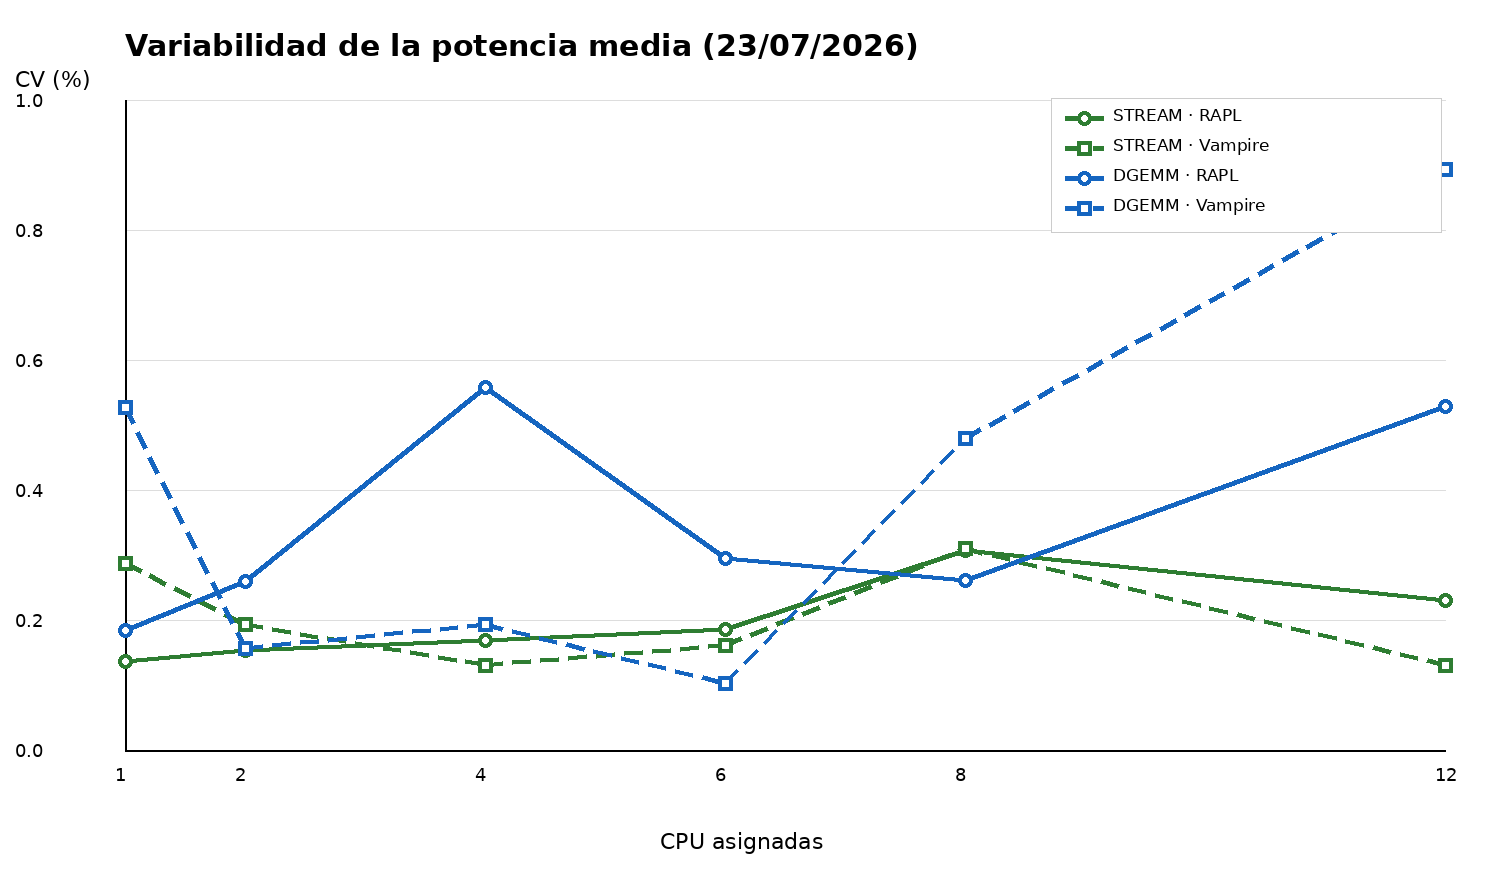
\includegraphics[width=0.94\textwidth]{imagenes/capitulo6/variabilidad_potencia.png}
    \caption{Coeficiente de variación de la potencia media RAPL y Vampire entre repeticiones.}
    \label{fig:variabilidad-potencia-cap6}
\end{figure}

\section{Resultados del programa de referencia Idle}
\label{sec:resultados-idle}

La ejecución de la prueba Idle tarda aproximadamente 120,5~s. RAPL registra 2,858~kJ, 23,703~W de potencia media y 28,323~W de potencia máxima. Vampire registra 10,926~kJ, 90,957~W de media y 93,4~W de máxima. La tabla~\ref{tab:idle-cap6} recoge estos valores.

\begin{table}[htbp]
    \centering
    \caption{Resultados de las fuentes interna y externa durante Idle.}
    \label{tab:idle-cap6}
    \begin{tabular}{lrr}
\hline
Métrica & RAPL & Vampire \\
\hline
Duración integrada (s) & 120.549 & 120.125 \\
Muestras & 104 & 24 \\
Energía (kJ) & 2.858 & 10.926 \\
Potencia media (W) & 23.703 & 90.957 \\
Potencia máxima (W) & 28.323 & 93.400 \\
\hline
\end{tabular}

\end{table}

La diferencia media de aproximadamente 67,3~W representa el consumo eléctrico observado externamente que no forma parte de los componentes leídos con RAPL, además de las diferencias propias de cada mecanismo de medida. Al existir una única ejecución Idle, este valor sirve como referencia y no se puede estimar su variabilidad.

\section{Resultados de STREAM}
\label{sec:resultados-stream}

El ancho de banda de memoria medido por STREAM pasa de ser 10,010~GB/s al ejecutar un proceso a 19,932~GB/s al ejecutar dos procesos en paralelo. Alcanza su mayor valor, 22,422~GB/s, con cuatro procesos, y después se mantiene alrededor de 22,2~GB/s cuando se ejecutan hasta doce procesos. La aceleración (speedup) es de 1,991 con el proceso p2, aumenta hasta 2,240 con el proceso p4 y se mantiene prácticamente igual, en 2,227, con el proceso p12. Esto muestra que el rendimiento mejora al principio, pero después se estabiliza..

La potencia obtenida a partir de los valores leídos por RAPL va de 74,018 W hasta 109,463~W. La potencia global calculada a partir de los valores obtenidos con Vampire van desde 156,282 W hasta 198,991~W. La energía medida con RAPL  toma los valores de 8,938 kJ a 13,555~kJ y de 18,832 kJ a 24,558~kJ cuando se obtiene a partir de las medidas con Vampire. Ambas fuentes presentan una evolución consistente respecto al aumento de los recursos asignados, sin cambios de tendencia en los valores registrados.

Las medidas asociadas a RAPL son crecientes, desde un 47,5~\% en el proceso \texttt{p1} hasta un 55,2~\% en el proceso \texttt{p12}. La diferencia entre el consumo global del sistema y las medidas internas se encuentran entre 9,89 kJ y 11,00~kJ. 

\section{Resultados de DGEMM}
\label{sec:resultados-dgemm}

El rendimiento obtenido con DGEMM aumenta de forma progresiva a medida que se incrementa el número de procesos: pasa de 0,668 GFLOP/s con un proceso a 1,378 GFLOP/s con dos, 2,406 GFLOP/s con cuatro, 2,856 GFLOP/s con seis, 3,291 GFLOP/s con ocho y 4,023 GFLOP/s con doce. Con doce procesos se alcanza una aceleración (speedup) de 6,022, lo que corresponde a una eficiencia paralela del 50,2~\%.

Al aumentar el número de procesos, ambas fuentes de medida muestran un incremento progresivo de la potencia media y de la energía consumida. En RAPL, la potencia media pasa de 74,870~W a 125,953~W, mientras que Vampire registra un aumento de 153,425~W a 221,225~W. De forma coherente, la energía acumulada crece desde 9,170 hasta 15,854~kJ en RAPL y desde 18,769 hasta 27,697~kJ en Vampire. Aunque la medida externa es superior en todos los casos, la proporción que representa RAPL respecto a Vampire aumenta del 48,9~\% al 57,2~\%. Al mismo tiempo, la diferencia absoluta entre ambas medidas también crece, pasando de 9,60 a 11,84~kJ.

Estos resultados indican que el aumento de la carga incrementa el consumo observado por ambas fuentes, pero no de forma idéntica, ya que RAPL y Vampire cubren ámbitos distintos del sistema.

La tabla~\ref{tab:resumen-activos} reúne los resultados medios de las cinco repeticiones para las dos cargas activas.

\begin{table}[htbp]
    \centering
    \caption{Rendimiento y medidas energéticas medias de STREAM y DGEMM.}
    \label{tab:resumen-activos}
    \resizebox{\textwidth}{!}{\begin{tabular}{lrrrrrrrr}
\hline
Benchmark & CPU & Rend. & Unidad & RAPL (W) & Vampire (W) & RAPL (kJ) & Vampire (kJ) & Cobertura (\%) \\
\hline
STREAM & 1 & 10.010 & GB/s & 74.02 & 156.28 & 8.94 & 18.83 & 47.5 \\
STREAM & 2 & 19.932 & GB/s & 85.18 & 170.53 & 10.30 & 20.57 & 50.1 \\
STREAM & 4 & 22.422 & GB/s & 91.92 & 178.78 & 11.15 & 21.63 & 51.5 \\
STREAM & 6 & 22.214 & GB/s & 95.40 & 182.98 & 11.64 & 22.27 & 52.3 \\
STREAM & 8 & 22.186 & GB/s & 99.91 & 188.27 & 12.28 & 23.04 & 53.3 \\
STREAM & 12 & 22.298 & GB/s & 109.46 & 198.99 & 13.56 & 24.56 & 55.2 \\
DGEMM & 1 & 0.668 & GFLOP/s & 74.87 & 153.43 & 9.17 & 18.77 & 48.9 \\
DGEMM & 2 & 1.378 & GFLOP/s & 85.88 & 166.46 & 10.58 & 20.42 & 51.8 \\
DGEMM & 4 & 2.406 & GFLOP/s & 97.91 & 180.19 & 12.11 & 22.19 & 54.6 \\
DGEMM & 6 & 2.856 & GFLOP/s & 106.09 & 192.00 & 13.12 & 23.65 & 55.5 \\
DGEMM & 8 & 3.291 & GFLOP/s & 114.12 & 203.22 & 14.20 & 25.18 & 56.4 \\
DGEMM & 12 & 4.023 & GFLOP/s & 125.95 & 221.23 & 15.85 & 27.70 & 57.2 \\
\hline
\end{tabular}
}
\end{table}

\section{Relación entre las medidas obtenidas con RAPL y Vampire}
\label{sec:resultados-vampire}

La Figura~\ref{fig:potencia-nucleos-cap6} compara la evolución de la potencia media registrada mediante RAPL y Vampire para STREAM y DGEMM al aumentar el número de CPU asignadas. Las cuatro series permiten observar tanto las diferencias entre los dos programas de referencia como la respuesta de las medidas interna y externa ante el incremento de recursos. Los valores obtenidos mediante Vampire son superiores a los registrados por RAPL debido al distinto alcance de ambas fuentes: RAPL considera los dominios \texttt{package} de los procesadores, mientras que Vampire mide el consumo eléctrico global del nodo.

\begin{figure}[htbp]
    \centering
    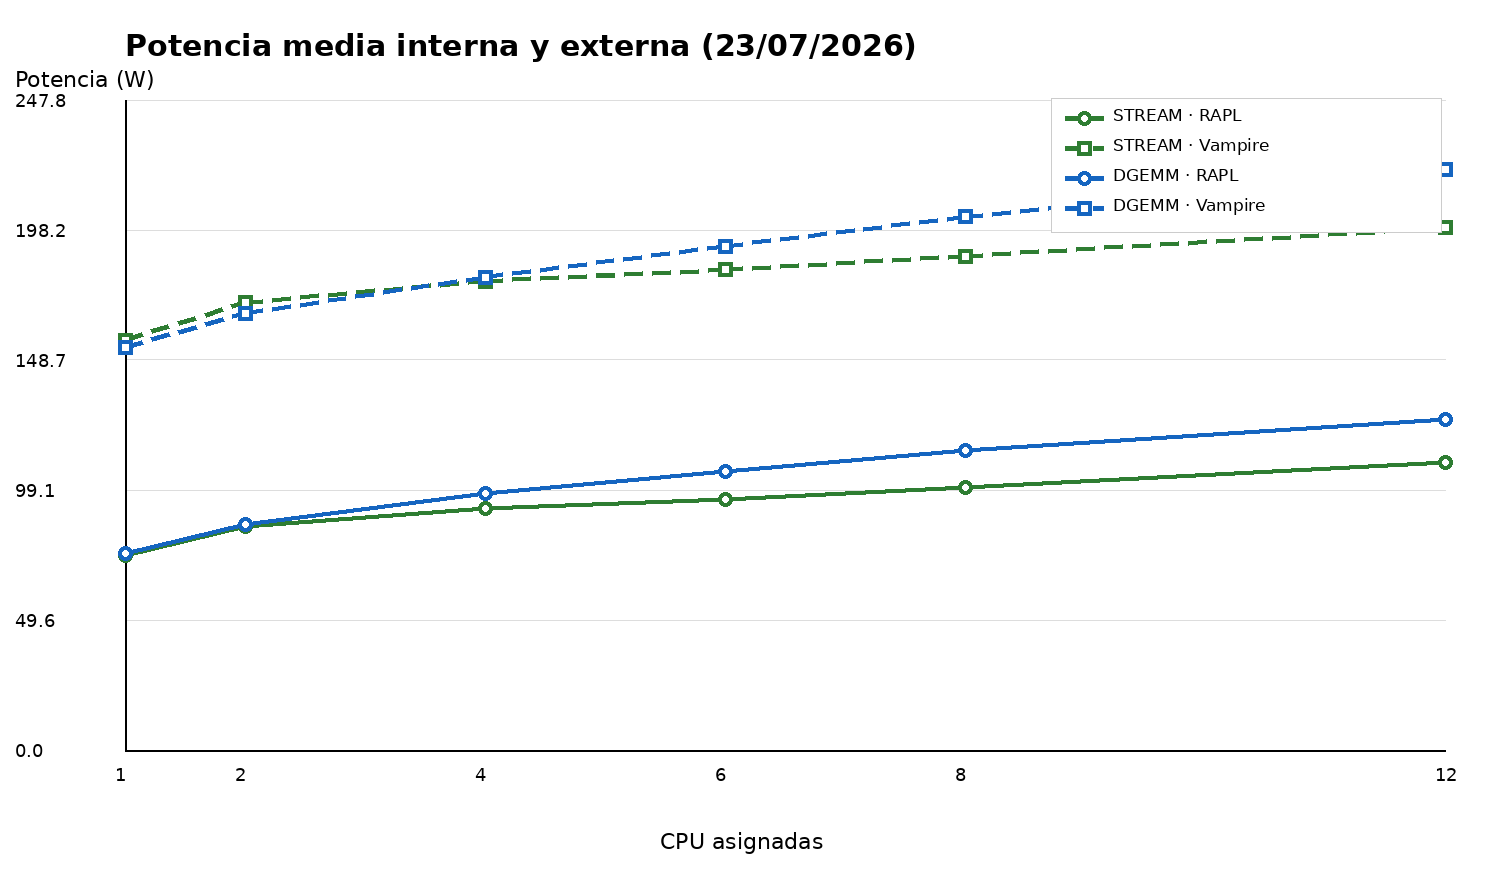
\includegraphics[width=0.94\textwidth]{imagenes/capitulo6/potencia_media_por_nucleos.png}
    \caption{Potencia media registrada mediante RAPL y Vampire para STREAM y DGEMM en función del número de CPU asignadas.}
    \label{fig:potencia-nucleos-cap6}
\end{figure}

La Figura~\ref{fig:energia-nucleos-cap6} presenta la misma comparación para la energía acumulada durante cada ejecución. Se representan las medidas de RAPL y Vampire para las seis configuraciones de STREAM y DGEMM.

\begin{figure}[htbp]
    \centering
    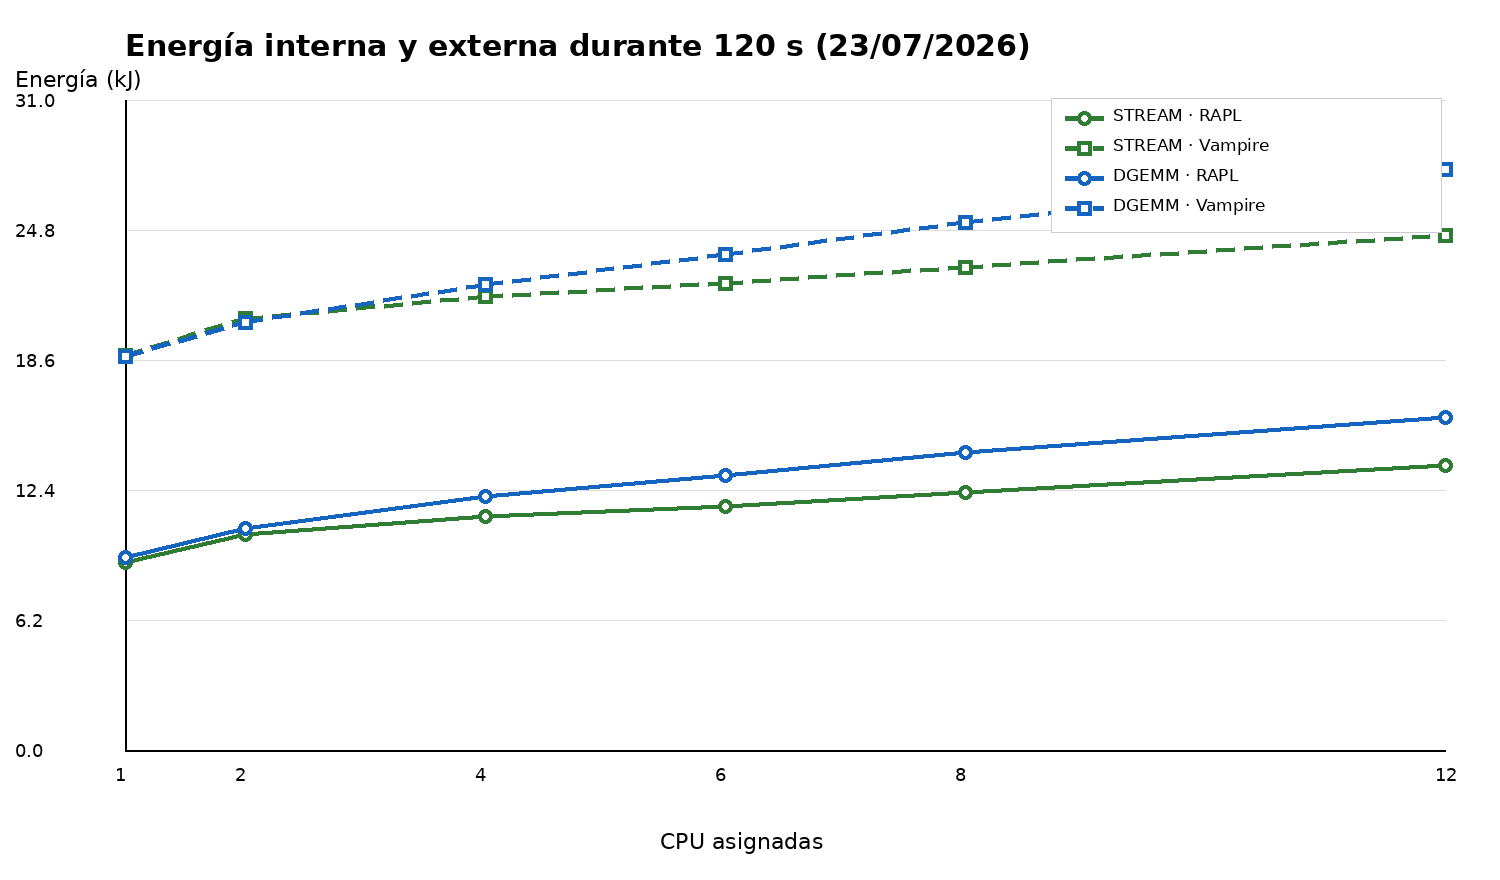
\includegraphics[width=0.94\textwidth]{imagenes/capitulo6/energia_por_nucleos.png}
    \caption{Energía registrada mediante RAPL y Vampire para STREAM y DGEMM en función del número de CPU asignadas, con una duración objetivo de 120~s por ejecución}
    \label{fig:energia-nucleos-cap6}
\end{figure}

Las cuatro series muestran un incremento de la energía al aumentar el número de CPU asignadas. La evolución es similar a la observada en la potencia media debido a que las ejecuciones tienen una duración objetivo aproximadamente constante. Vampire registra valores superiores a RAPL en todas las configuraciones, mientras que DGEMM presenta un crecimiento más acusado que STREAM al aumentar el número de procesos. Estas diferencias se interpretan considerando que ambas fuentes miden dominios energéticos distintos.

La Tabla~\ref{tab:vampire-cap6} muestra la diferencia entre la energía registrada mediante RAPL y Vampire, así como la relación porcentual entre ambas medidas. En todas las ejecuciones analizadas, Vampire registra valores superiores a RAPL, como corresponde al distinto alcance de cada fuente: RAPL considera los dominios \texttt{package} de los procesadores, mientras que Vampire mide el consumo eléctrico global del nodo. Además, las medidas externas presentan una baja variabilidad entre repeticiones y aumentan de forma coherente al incrementar la carga. Estos resultados permiten comprobar que la integración de Vampire proporciona medidas consistentes durante la campaña, aunque no permiten considerar RAPL y Vampire como instrumentos equivalentes ni constituyen una calibración de ninguno de ellos.

\begin{table}[htbp]
    \centering
    \caption{Energía consumida medida con RAPL y Vampire.}
    \label{tab:vampire-cap6}
    \resizebox{\textwidth}{!}{%
        \begin{tabular}{lrrrr}
\hline
Benchmark & CPU & Vampire--RAPL (kJ) & RAPL/Vampire (\%) & Vampire/RAPL \\
\hline
STREAM & 1 & 9.89 & 47.5 & 2.107 \\
STREAM & 2 & 10.27 & 50.1 & 1.997 \\
STREAM & 4 & 10.48 & 51.5 & 1.940 \\
STREAM & 6 & 10.63 & 52.3 & 1.913 \\
STREAM & 8 & 10.76 & 53.3 & 1.876 \\
STREAM & 12 & 11.00 & 55.2 & 1.812 \\
DGEMM & 1 & 9.60 & 48.9 & 2.047 \\
DGEMM & 2 & 9.83 & 51.8 & 1.929 \\
DGEMM & 4 & 10.08 & 54.6 & 1.833 \\
DGEMM & 6 & 10.53 & 55.5 & 1.803 \\
DGEMM & 8 & 10.98 & 56.4 & 1.773 \\
DGEMM & 12 & 11.84 & 57.2 & 1.747 \\
\hline
\end{tabular}
%
    }
\end{table}

\section{Análisis de escalabilidad}
\label{sec:analisis-escalabilidad}
A continuación se analiza cómo evoluciona el comportamiento de los programas de referencia al aumentar el número de CPU asignadas. Para ello se estudian el rendimiento, la potencia y la energía obtenidos para los distintos perfiles de ejecución, así como la eficiencia de escalado y la eficiencia energética. El objetivo es determinar hasta qué punto el incremento de recursos se traduce en una mejora efectiva del rendimiento y cómo varía, al mismo tiempo, el consumo energético.

\subsection{Rendimiento}

La figura~\ref{fig:speedup-nucleos-cap6} muestra la evolución de la aceleración (speedup) de los programas de pruebas, STREAM y DGEMM, al aumentar el número de CPUs asignadas. En el eje horizontal aparece el número de CPU asignadas y en el vertical la aceleración (speedup). La línea gris representa la escalabilidad ideal, es decir,  si se duplicaran los recursos, el rendimiento también debería duplicarse. STREAM mejora claramente al pasar de uno a dos procesos, pero a partir de 4 procesos el aumento es mucho menor y finalmente el rendimiento prácticamente se estabiliza. Esto indica que añadir más CPUs no supone una mejora significativa, probablemente porque se alcanza una limitación asociada al ancho de banda de memoria. DGEMM continúa aumentando su rendimiento conforme se incrementan las CPUs. Sin embargo, su crecimiento también está por debajo del ideal: con 12 CPUs alcanza una acelaración de aproximadamente 6, en lugar de 12. Por tanto, sigue aprovechando los recursos adicionales, aunque con una eficiencia cada vez menor. Ambos programas permanecen por debajo de la escalabilidad ideal, siendo esta diferencia especialmente acusada en STREAM. 

\begin{figure}[htbp]
    \centering
    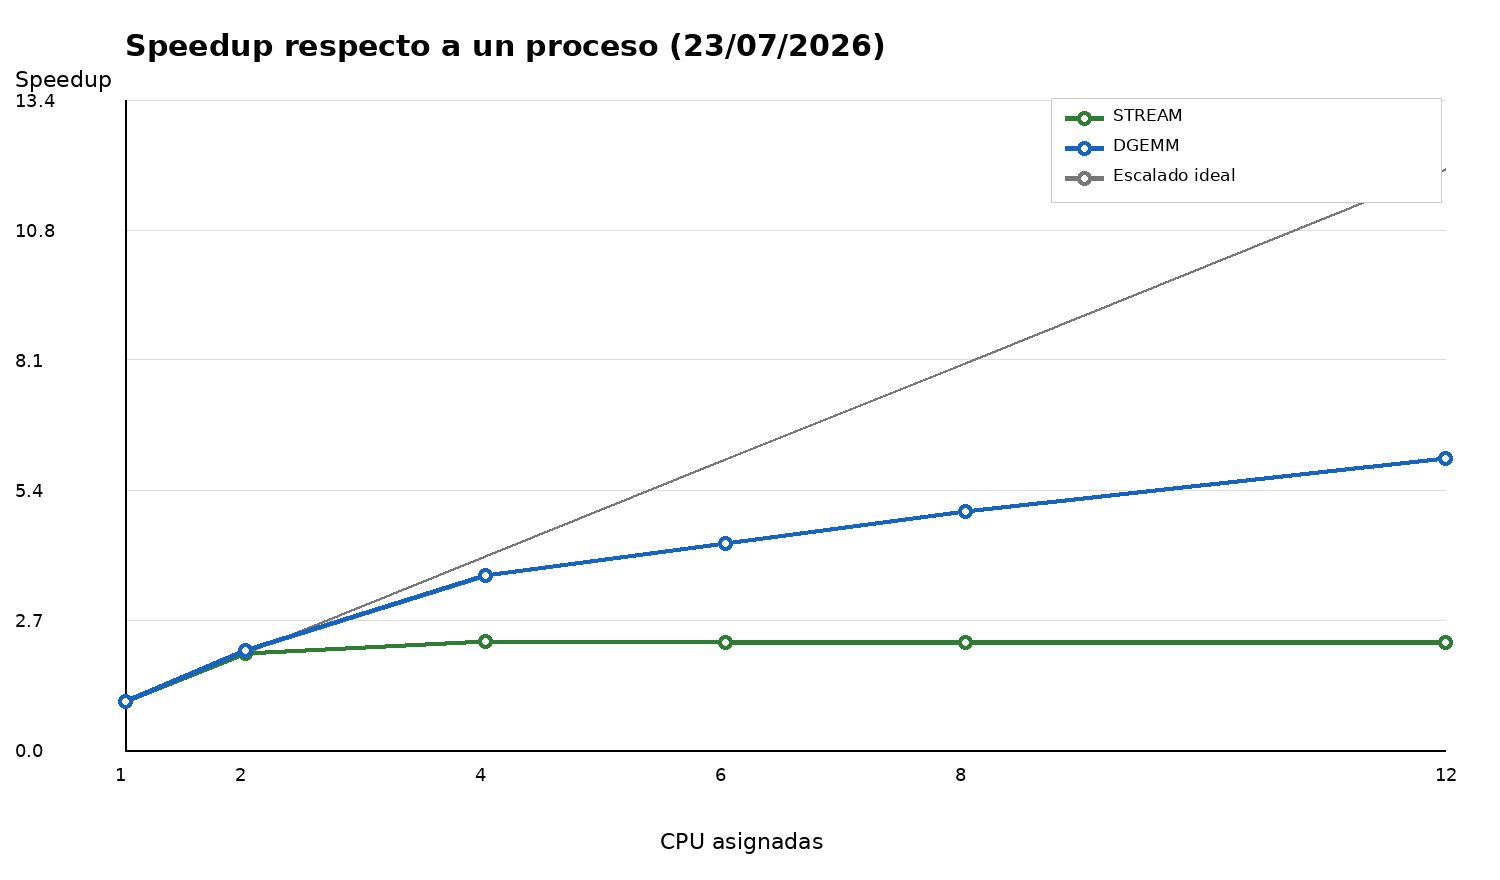
\includegraphics[width=0.92\textwidth]{imagenes/capitulo6/speedup_por_nucleos.png}
    \caption{Aceleración de STREAM y DGEMM con el número de CPUs.}
    \label{fig:speedup-nucleos-cap6}
\end{figure}

\subsection{Potencia y energía}

La figura 6.5 muestra cómo evoluciona en el tiempo la potencia medida con RAPL durante varias ejecuciones de STREAM y DGEMM, con 1 proceso (p1) y con 12 procesos (p12).

Las series temporales obtenidas con RAPL muestran un consumo de potencia estable durante la mayor parte de las ejecuciones. Con un proceso, STREAM y DGEMM se mantienen en torno a 50 W, mientras que con doce procesos la potencia aumenta hasta aproximadamente 95 W. En STREAM, aumentar de cuatro a doce procesos apenas modifica el rendimiento, pero eleva la energía obtenida con RAPL un 21,6~\% y la energía obtenida con Vampire un 13,5~\%

Además, el gráfico muestra que el número de procesos tiene mucha más influencia sobre la potencia que el tipo de programa, ya que STREAM y DGEMM presentan valores bastante similares cuando utilizan el mismo número de procesos. Sin embargo, esto no significa que tengan el mismo rendimiento: como se veía en el gráfico anterior, DGEMM aprovecha mucho mejor el aumento de procesos que STREAM. Al finalizar las ejecuciones se observa una caída brusca de la potencia, correspondiente a la finalización de la ejecución.  
\begin{figure}[htbp]
    \centering
    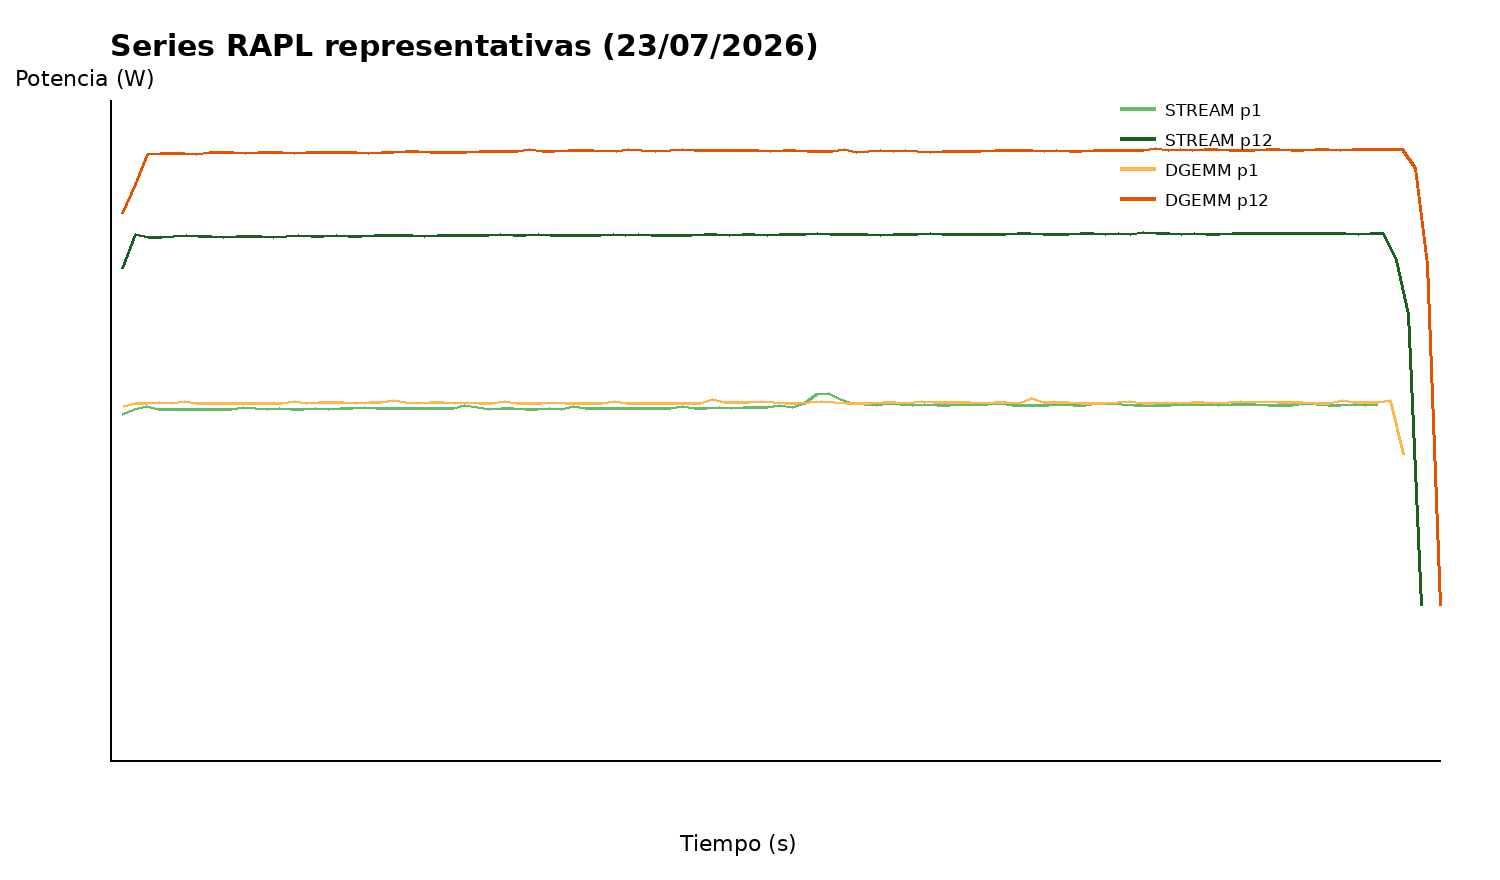
\includegraphics[width=0.94\textwidth]{imagenes/capitulo6/series_rapl_representativas.png}
    \caption{Evolución temporal de la potencia medida con RAPL  para STREAM y DGEMM.}
    \label{fig:series-rapl-cap6}
\end{figure}

\subsection{Eficiencia energética}

La eficiencia energética mide el rendimiento que se obtiene por cada unidad de energía o potencia consumida. En este trabajo se calcula dividiendo el trabajo total realizado por la energía consumida durante la ejecución para STREAM y se expresa en bytes/j, mientras que para DGEMM se expresa en operaciones/J

La evolución de la eficiencia energética muestra comportamientos claramente diferentes para STREAM y DGEMM. En ambos casos, el perfil de un proceso se utiliza como referencia, por lo que un valor superior a 1 indica que la cantidad de trabajo realizada por cada julio consumido ha aumentado respecto a dicha configuración.

En STREAM, la eficiencia energética mejora al pasar de uno a dos y cuatro procesos, alcanzando su valor máximo en el perfil de cuatro procesos. A partir de este punto, la tendencia se invierte y la eficiencia disminuye progresivamente al utilizar seis, ocho y doce procesos. Este comportamiento está relacionado con la evolución del rendimiento observada anteriormente: STREAM aumenta considerablemente su rendimiento hasta cuatro procesos, pero a partir de ese perfil permanece prácticamente estable. Sin embargo, la energía consumida continúa aumentando al incorporar más recursos. En consecuencia, los perfiles superiores a cuatro procesos consumen más energía sin producir un incremento proporcional de la cantidad de datos procesados.

DGEMM presenta un comportamiento diferente. Su eficiencia energética aumenta de forma sostenida al incrementar el número de procesos y alcanza su valor máximo con doce. En este caso, el aumento del consumo energético producido al utilizar más recursos se acompaña de un crecimiento suficiente del rendimiento, por lo que la cantidad de operaciones realizadas por julio continúa mejorando. Esto indica que, dentro del rango analizado, DGEMM aprovecha de forma más efectiva el incremento de los recursos de cálculo que STREAM.

Estos resultados muestran que la configuración energéticamente más eficiente depende del tipo de carga. En STREAM, aumentar el número de procesos más allá de cuatro deja de resultar favorable desde el punto de vista de la eficiencia energética, mientras que DGEMM continúa beneficiándose del aumento de recursos hasta el máximo estudiado. Por tanto, asignar un mayor número de CPU no garantiza por sí mismo una utilización más eficiente de la energía: es necesario considerar conjuntamente el aumento del rendimiento y el incremento del consumo producido por cada configuración.

La Figura~\ref{fig:eficiencia-energetica-cap6} permite observar esta diferencia de forma directa. Mientras que STREAM presenta un máximo seguido de una disminución progresiva, DGEMM mantiene una tendencia creciente. Esta diferencia refuerza la idea de que no existe un único perfil óptimo para todas las cargas y que la selección de recursos puede variar en función del objetivo perseguido, ya sea maximizar el rendimiento, limitar el consumo o aumentar la cantidad de trabajo realizada por unidad de energía.

\begin{figure}[htbp]
    \centering
    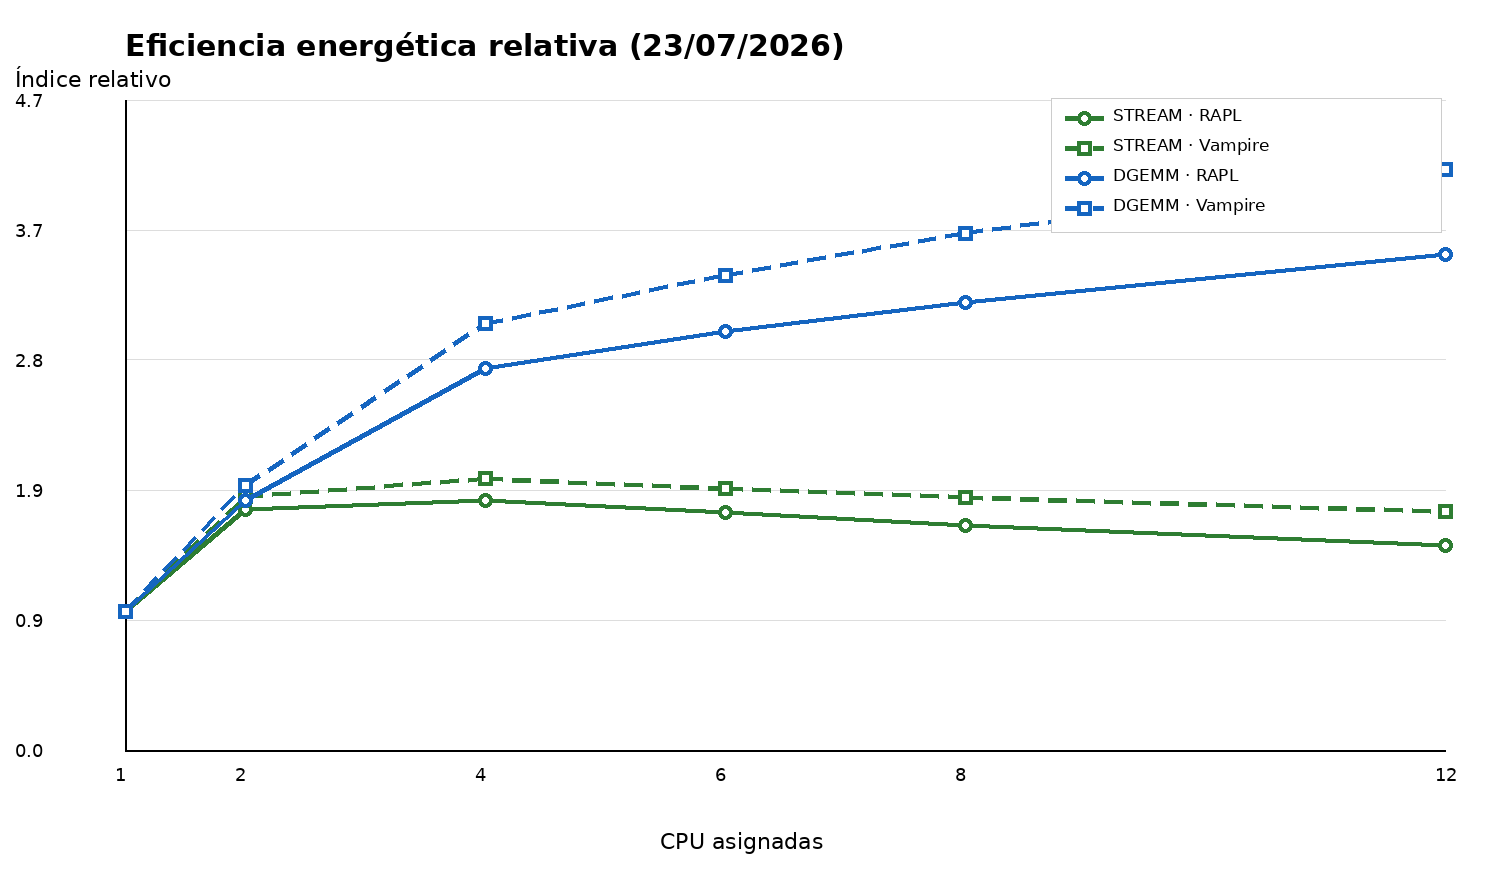
\includegraphics[width=0.92\textwidth]{imagenes/capitulo6/eficiencia_energetica_relativa.png}
    \caption{Evolución de la eficiencia energética relativa con el número de procesos.}
    \label{fig:eficiencia-energetica-cap6}
\end{figure}

La tabla~\ref{tab:escalabilidad-cap6} compara cómo evolucionan la aceleración, la eficiencia paralela y la eficiencia energética de STREAM y DGEMM al aumentar el número de CPU asignadas.

\begin{table}[htbp]
    \centering
    \caption{Indicadores de escalabilidad y eficiencia energética para STREAM y DGEMM.}
    \label{tab:escalabilidad-cap6}
    \resizebox{\textwidth}{!}{\begin{tabular}{lrrrrr}
\hline
Benchmark & CPU & Speedup & Eficiencia paralela (\%) & Efic. RAPL & Efic. Vampire \\
\hline
STREAM & 1 & 1.000 & 100.0 & 1.000 & 1.000 \\
STREAM & 2 & 1.991 & 99.6 & 1.728 & 1.823 \\
STREAM & 4 & 2.240 & 56.0 & 1.797 & 1.951 \\
STREAM & 6 & 2.219 & 37.0 & 1.706 & 1.879 \\
STREAM & 8 & 2.216 & 27.7 & 1.618 & 1.817 \\
STREAM & 12 & 2.227 & 18.6 & 1.474 & 1.715 \\
DGEMM & 1 & 1.000 & 100.0 & 1.000 & 1.000 \\
DGEMM & 2 & 2.062 & 103.1 & 1.792 & 1.901 \\
DGEMM & 4 & 3.601 & 90.0 & 2.745 & 3.067 \\
DGEMM & 6 & 4.275 & 71.3 & 3.009 & 3.417 \\
DGEMM & 8 & 4.926 & 61.6 & 3.222 & 3.720 \\
DGEMM & 12 & 6.022 & 50.2 & 3.565 & 4.177 \\
\hline
\end{tabular}
}
\end{table}

\section{Análisis estadístico}
\label{sec:estadistica-cap6}
En los siguientes subapartados se detalla el análisis estadístico llevado a cabo con los datos obtenidos.  Para ello se estudia, en primer lugar, la variabilidad entre repeticiones de una misma configuración con el objetivo de comprobar la estabilidad de las medidas. A continuación, se analizan las relaciones entre las principales métricas de rendimiento y consumo energético mediante medidas de correlación. Finalmente, se comparan los comportamientos observados entre los distintos programas de referencia y perfiles de ejecución, tratando de identificar tendencias consistentes y diferencias relevantes entre configuraciones.

\subsection{Estadística descriptiva y variabilidad}

Las medias y los coeficientes de variación muestran que energía y potencia son más estables que el rendimiento DGEMM. La mayor dispersión energética es 0,65~\% para RAPL y 1,04~\% para Vampire. La potencia media no supera 0,57~\% en RAPL ni 0,91~\% en Vampire. Estas cifras permiten distinguir los perfiles sin que la variación entre repeticiones domine las tendencias.

\subsection{Matriz de correlación}

Con el objetivo de estudiar si existe una relación entre las principales variables registradas durante la campaña, se ha calculado una matriz de correlación. Este tipo de matriz permite comparar varias variables entre sí y resumir, en una única representación, hasta qué punto dos magnitudes tienden a variar de forma conjunta.

Para cuantificar esta relación se utiliza el coeficiente de correlación de Pearson. Este coeficiente toma valores comprendidos entre \(-1\) y \(1\). Un valor próximo a \(1\) indica que, cuando una variable aumenta, la otra tiende también a aumentar. Un valor próximo a \(-1\) indica una evolución en sentido contrario, mientras que un valor cercano a \(0\) indica que no existe una relación lineal clara entre ambas variables. La correlación mide, por tanto, el grado de asociación lineal entre dos magnitudes, pero no permite afirmar por sí sola que una sea la causa de la otra.

La matriz de correlación se ha utilizado en este trabajo porque permite comprobar de forma sencilla si los cambios introducidos en las configuraciones experimentales se reflejan de manera consistente en las métricas de consumo. En particular, resulta de interés estudiar la relación entre el número de CPU asignadas y la energía registrada, así como comprobar si las medidas obtenidas mediante RAPL y Vampire presentan una evolución similar a lo largo de las distintas ejecuciones.

Para este análisis se consideran las 60 ejecuciones correspondientes a las cargas activas, STREAM y DGEMM. La ejecución Idle no se incluye, ya que constituye una única referencia basal y no forma parte de los perfiles repetidos utilizados para estudiar la variación con el número de CPU.

La Figura~\ref{fig:matriz-correlacion-cap6} muestra los valores obtenidos. El número de CPU asignadas presenta una correlación de \(0{,}911\) con la energía registrada mediante RAPL y de \(0{,}928\) con la energía medida por Vampire. Ambos valores son elevados y positivos, lo que indica que, dentro de las configuraciones analizadas, el aumento del número de CPU está asociado generalmente a un incremento de la energía consumida.

La correlación más elevada se observa entre las energías registradas mediante RAPL y Vampire, con un valor de \(r=0{,}995\). Este resultado indica que ambas magnitudes siguen una evolución lineal muy similar entre las diferentes ejecuciones: cuando aumenta la energía registrada mediante RAPL, también tiende a aumentar la energía medida externamente por Vampire.

Sin embargo, este resultado no significa que ambas herramientas estén midiendo la misma parte del sistema. RAPL registra la energía correspondiente a los dominios \texttt{package} de los procesadores, mientras que Vampire mide el consumo eléctrico global del nodo. Por tanto, la elevada correlación debe interpretarse como una similitud en la evolución de ambas medidas ante los cambios de carga y de recursos, y no como una equivalencia entre los dos sistemas de medición.

\begin{figure}[H]
    \centering
    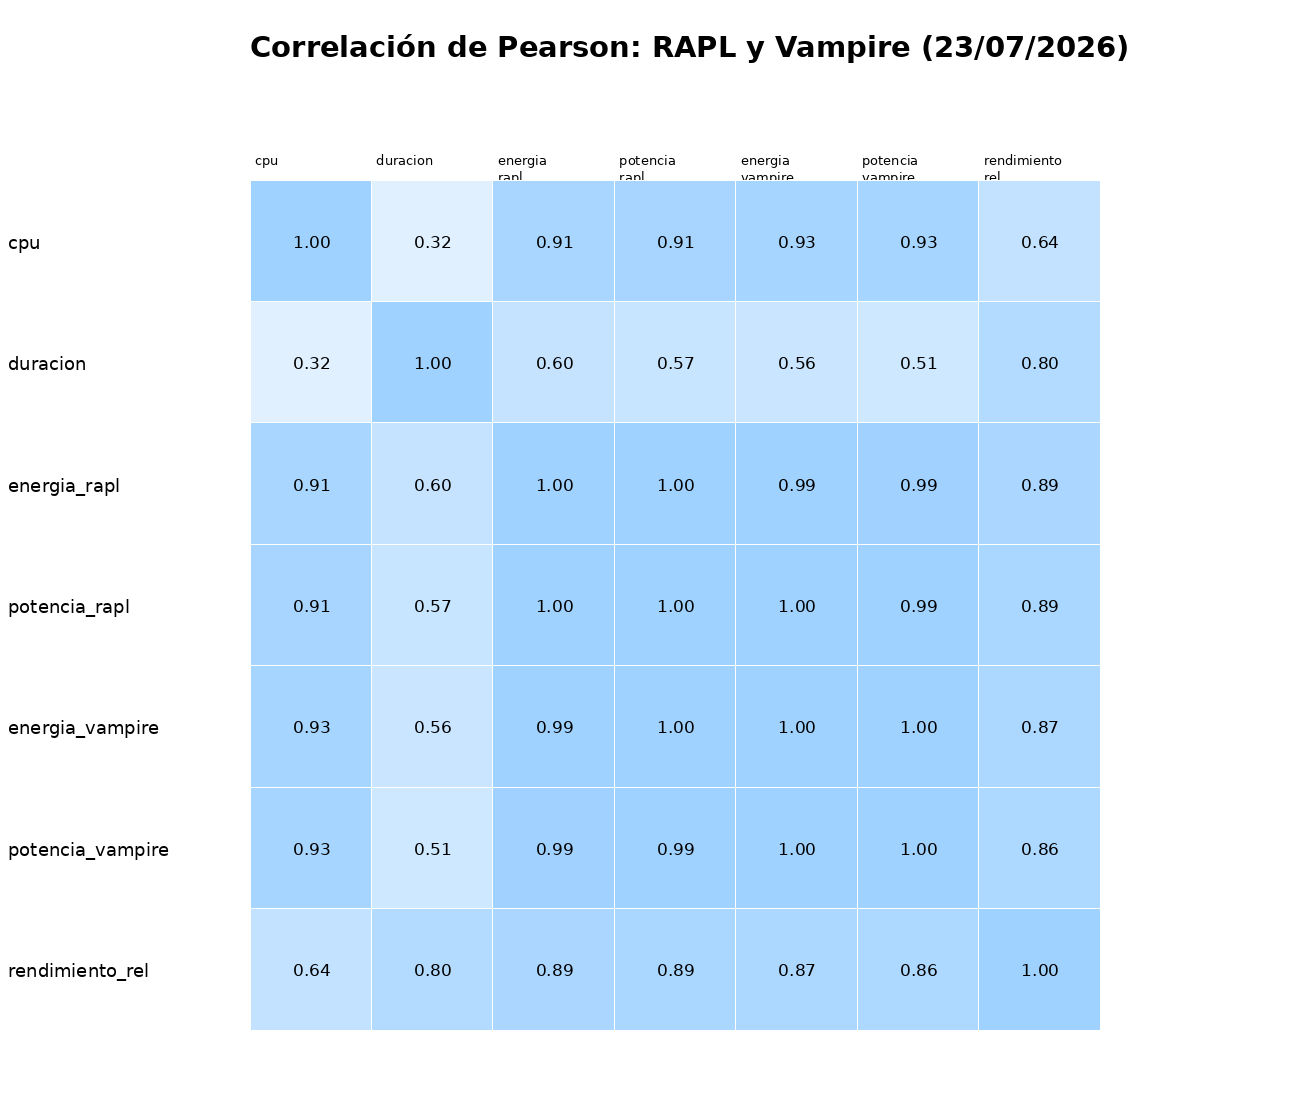
\includegraphics[width=0.90\textwidth]{imagenes/capitulo6/matriz_correlacion.png}
    \caption{Matriz de correlación de Pearson para métricas internas, externas y de rendimiento.}
    \label{fig:matriz-correlacion-cap6}
\end{figure}

La correlación entre energía y potencia es parcialmente estructural porque las duraciones son próximas. Del mismo modo, el rendimiento relativo deriva del trabajo y del tiempo. La matriz se utiliza para controlar la coherencia y para detectar la existencia de variables redundantes, no para demostrar causalidad.

\subsection{Selección e interpretación de métricas}

Para caracterizar cada ejecución se han seleccionado métricas relacionadas con tres aspectos principales: el tiempo de ejecución, el rendimiento obtenido y el consumo energético. Además, se conservan algunas variables auxiliares destinadas a comprobar la calidad de las medidas. La elección de estas métricas permite analizar no solo cuánto consume una configuración, sino también cuánto trabajo realiza y cómo evoluciona su comportamiento al aumentar los recursos asignados.

La \textbf{duración} representa el tiempo durante el que se ejecuta el programa de referencia. En STREAM y DGEMM se utiliza una ventana objetivo de aproximadamente 120~s, aunque se registra el tiempo real de cada ejecución. Esta métrica permite comprobar que las distintas pruebas se han desarrollado durante intervalos comparables y sirve también para calcular las tasas de rendimiento.

El \textbf{rendimiento} expresa la cantidad de trabajo realizada por unidad de tiempo. Su definición depende del programa de referencia. En STREAM se calcula a partir de la cantidad total de datos procesados por todos los procesos y se expresa en GB/s. En DGEMM se utiliza el número de operaciones en coma flotante realizadas por unidad de tiempo y se expresa en GFLOP/s. Para obtener el rendimiento agregado se suma el trabajo realizado por todos los procesos y se divide entre la mayor duración registrada entre ellos, ya que los procesos se ejecutan de forma concurrente.

La \textbf{energía} indica la cantidad total de energía consumida durante la ventana analizada. En RAPL se obtiene sumando los incrementos de energía calculados entre lecturas consecutivas de los contadores \texttt{package}. En Vampire se calcula a partir de las muestras de potencia registradas durante la ejecución, integrándolas sobre el intervalo temporal correspondiente al programa de referencia. La energía se expresa en julios o kilojulios y permite estudiar cómo aumenta el consumo total al modificar el número de recursos utilizados.

La \textbf{potencia media} representa la velocidad media a la que se consume energía durante una ejecución y se expresa en vatios. En RAPL se obtiene a partir de la energía consumida entre muestras consecutivas y del tiempo transcurrido entre ellas. En Vampire se calcula a partir de las muestras de potencia correspondientes a la misma ventana temporal. Esta métrica permite comparar la intensidad del consumo entre configuraciones sin depender únicamente de la energía total acumulada.

La \textbf{potencia máxima} corresponde al mayor valor de potencia observado durante una ejecución. Su inclusión permite detectar los niveles máximos alcanzados durante las cargas, aunque debe interpretarse con precaución. RAPL y Vampire utilizan intervalos de muestreo diferentes, por lo que un sistema con mayor frecuencia de adquisición tiene más posibilidades de registrar variaciones breves de potencia. Por este motivo, la potencia máxima se utiliza como información complementaria y no para realizar una comparación directa muestra a muestra entre ambas fuentes.

También se calcula la \textbf{diferencia de energía entre Vampire y RAPL}, definida como:

\[
\Delta E_{\mathrm{ext-int}} =
E_{\mathrm{Vampire}} - E_{\mathrm{RAPL}}.
\]

donde \(E_{\mathrm{Vampire}}\) es la energía medida externamente para el nodo completo y \(E_{\mathrm{RAPL}}\) la energía registrada en los dominios \texttt{package} seleccionados. Esta diferencia permite cuantificar cuánto mayor es la medida externa respecto a la interna. No debe interpretarse como el consumo exacto del resto de componentes del nodo, ya que ambas herramientas presentan alcances de medida diferentes y la diferencia no permite realizar una descomposición energética por componentes.

Para estudiar la relación entre ambas fuentes se calcula además la \textbf{cobertura RAPL}, definida como:

\[
C_{\mathrm{RAPL}} =
100\,
\frac{E_{\mathrm{RAPL}}}
     {E_{\mathrm{Vampire}}}.
\]

Esta métrica expresa qué porcentaje de la energía registrada externamente por Vampire representa la energía medida mediante los dominios RAPL seleccionados. Por ejemplo, una cobertura del 50~\% indica que la energía registrada mediante RAPL equivale aproximadamente a la mitad de la energía medida externamente durante esa ejecución. Este porcentaje no debe interpretarse como la fracción exacta del consumo del nodo atribuible a la CPU, sino como una relación entre los alcances de las dos fuentes de medida utilizadas en el trabajo.

Por último, el \textbf{número de muestras} y el \textbf{estado de la captura} se conservan como indicadores de calidad. El número de muestras permite comprobar que la ejecución contiene suficientes observaciones para cubrir el intervalo analizado, mientras que el estado de captura indica si el proceso de adquisición finalizó correctamente. Estas variables no se utilizan como resultados energéticos principales, pero permiten detectar ejecuciones incompletas o potencialmente inválidas antes de incorporarlas al análisis.

En conjunto, estas métricas permiten estudiar cada configuración desde distintas perspectivas. La duración y el rendimiento describen el trabajo realizado, la energía y la potencia caracterizan el consumo, la diferencia y la cobertura permiten analizar la relación entre las medidas internas y externas, y los indicadores de calidad ayudan a asegurar que los datos utilizados en el análisis proceden de ejecuciones correctamente registradas.

\section{Evaluación global del sistema}
\label{sec:evaluacion-global-cap6}

En los siguientes apartados se realiza una valoración conjunta del funcionamiento del sistema a partir de los resultados obtenidos en la campaña final. Para ello se consideran tanto la calidad y consistencia de las medidas como la capacidad de la plataforma para distinguir el comportamiento de las distintas cargas y configuraciones. El objetivo es comprobar si la infraestructura desarrollada cumple de forma adecuada su función como herramienta de medición, análisis y comparación del consumo energético en HPMoon.

\subsection{Funcionalidad}

De los resultados obtenidos tras las ejecuciones se puede deducir que el sistema es capaz de completar y coordinar las 61 ejecuciones mediante SLURM, obtener medidas energéticas de los dominios \texttt{package} de los procesadores mediante RAPL y del consumo eléctrico global del nodo mediante Vampire, procesar estos datos, conservar los resultados y publicar las métricas asociadas a un mismo identificador de ejecución (\texttt{run\_id}). Además, el sistema organiza estas tareas en etapas diferenciadas: la configuración define las condiciones de la prueba, la ejecución lanza el programa de referencia, la adquisición recoge las medidas, el almacenamiento conserva los resultados, la publicación envía las métricas al sistema de monitorización y el análisis procesa posteriormente los datos obtenidos. Esta organización facilita revisar o modificar cada etapa sin alterar necesariamente el resto del flujo.

\subsection{Coherencia}

En este trabajo, la coherencia de los resultados se entiende como la consistencia entre los datos almacenados, los valores recalculados a partir de las muestras originales y la evolución observada al modificar las condiciones de ejecución. Evaluar esta coherencia es importante porque permite comprobar que el sistema de medida y procesamiento no introduce discrepancias internas y que las métricas obtenidas responden de forma estable a los cambios de carga.

Para ello se han realizado varias comprobaciones. En primer lugar, los valores agregados de energía y potencia se han recalculado a partir de los archivos CSV originales y se ha verificado que coinciden con los resultados almacenados. En segundo lugar, se ha comprobado que tanto las medidas obtenidas mediante RAPL como las registradas por Vampire presentan una evolución consistente al aumentar la carga y una baja dispersión entre repeticiones equivalentes. Finalmente, la relación entre ambas medidas se interpreta teniendo en cuenta su distinto alcance: RAPL registra la energía asociada a los dominios \texttt{package} de los procesadores, mientras que Vampire mide el consumo eléctrico global del nodo.

\subsection{Repetibilidad y utilidad}

La repetibilidad se evalúa mediante la realización de varias ejecuciones bajo una misma configuración. Su análisis permite comprobar hasta qué punto los resultados se mantienen estables cuando se repite una prueba en condiciones equivalentes y detectar posibles ejecuciones anómalas. Para las configuraciones activas de STREAM y DGEMM se realizaron cinco repeticiones por perfil, como compromiso entre disponer de varias observaciones para estimar la variabilidad y mantener una duración asumible de la campaña. A partir de estas repeticiones se calcularon medidas de dispersión, cuyos resultados muestran una variabilidad reducida en las principales magnitudes energéticas.

También se evalúa la capacidad del sistema para distinguir diferentes comportamientos de carga. Los programas utilizados representan situaciones distintas: Idle sirve como referencia de baja actividad, STREAM genera una carga orientada principalmente al subsistema de memoria y DGEMM una carga intensiva de cálculo. Los resultados permiten observar diferencias entre ambos programas al aumentar los recursos asignados. STREAM alcanza una zona en la que añadir más procesos apenas incrementa el rendimiento, mientras que DGEMM continúa mejorando dentro del rango estudiado.

Finalmente, la combinación de las métricas de rendimiento y energía permite estudiar si el aumento de los recursos asignados produce una mejora proporcional del trabajo realizado. Este análisis se realiza directamente sobre los datos almacenados de cada ejecución, mientras que los paneles de Grafana se utilizan como herramienta complementaria de visualización y supervisión.

\subsection{Alcance de la evaluación}
\label{sec:alcance-cap6}

Los resultados presentados en este capítulo deben interpretarse dentro de las condiciones concretas en las que se ha realizado la campaña experimental. La evaluación se ha llevado a cabo sobre un único nodo de cómputo de HPMoon, \texttt{compute-0-4}, utilizando tres programas de referencia y seis perfiles de ejecución para las cargas activas. STREAM y DGEMM se ejecutaron durante una ventana objetivo de 120~s y con cinco repeticiones por perfil, mientras que Idle se utilizó como referencia basal mediante una única ejecución.

Esta configuración se eligió con el objetivo de mantener un experimento suficientemente controlado y asumible en duración, evitando introducir simultáneamente un número elevado de variables. Por este motivo, el estudio se centra principalmente en analizar cómo varían el rendimiento y el consumo energético al modificar el número de procesos asignados a cada carga.

Otros factores que pueden influir en el comportamiento del sistema no se estudian de forma específica en esta campaña. Entre ellos se encuentran la distribución de procesos y memoria dentro de la arquitectura NUMA, el uso de SMT, la afinidad física exacta sobre los núcleos, la frecuencia efectiva del procesador, la temperatura y la actividad de fondo del sistema. Aunque estos factores pueden afectar a las medidas, incorporarlos como variables experimentales habría ampliado considerablemente el número de configuraciones necesarias y dificultado la interpretación de los resultados obtenidos.

El uso de un único nodo también limita la generalización de las conclusiones. Los resultados describen el comportamiento observado en la configuración hardware evaluada y no deben extrapolarse directamente a otros nodos, procesadores o arquitecturas del clúster. Del mismo modo, los programas utilizados representan tres tipos concretos de carga y no pretenden reproducir toda la diversidad de aplicaciones que pueden ejecutarse en un entorno HPC.

Por último, las medidas obtenidas mediante RAPL y Vampire corresponden a ámbitos diferentes del sistema. RAPL registra la energía asociada a los dominios \texttt{package} de los procesadores, mientras que Vampire mide el consumo eléctrico global del nodo. Por este motivo, sus valores se analizan de forma complementaria y no como dos medidas equivalentes de una misma magnitud.

Estas limitaciones no invalidan los resultados obtenidos, sino que delimitan el alcance de las conclusiones que pueden extraerse de la campaña. La discusión global de estos resultados, junto con las posibles ampliaciones destinadas a abordar estas limitaciones, se desarrolla en el capítulo~\ref{chap:conclusiones}.

\subsection{Síntesis de los resultados}
\label{sec:sintesis-cap6}

La campaña realizada permite comprobar que la infraestructura desarrollada es capaz de ejecutar de forma automatizada las distintas configuraciones experimentales, conservar las medidas y metadatos asociados y generar resultados trazables y repetibles dentro de las condiciones estudiadas. Los datos obtenidos permiten distinguir el comportamiento de las cargas estudiadas y muestran diferencias claras en la evolución del rendimiento y del consumo al aumentar los recursos asignados.

La interpretación de estos resultados, sus implicaciones dentro del objetivo general del trabajo y las líneas de continuación que pueden plantearse a partir de las limitaciones identificadas se desarrollan en el capítulo~\ref{chap:conclusiones}.

\chapter{Planificación y gestión del proyecto}
\label{chap:planificacion}

\section{Metodología de desarrollo}
\label{sec:planificacion-metodologia}

El desarrollo de este trabajo ha seguido un enfoque incremental e iterativo combinado con una metodología experimental, sin adoptar formalmente Scrum, Kanban u otra metodología de trabajo ágil. La organización del trabajo se ha basado en el despliegue y la configuración de los servicios que componen la plataforma, su prueba en el clúster HPMoon y la revisión de las decisiones a partir de los resultados obtenidos.

El proceso no fue estrictamente lineal. Para automatizar un conjunto de pruebas fue necesario disponer previamente de un muestreador y de cargas ejecutables; a su vez, las primeras ejecuciones pusieron de manifiesto limitaciones que no podrían detectarse mediante pruebas locales. La integración con SLURM, los servicios remotos y el uso del medidor Vampire obligaron a alternar el análisis del entorno, la implementación, y el diagnóstico, ya que algunas incidencias solo podían detectarse al ejecutar el sistema en HPMoon. Tras cada corrección fue necesario repetir las ejecuciones para comprobar que el problema se había resuelto y que el flujo completo seguía funcionando correctamente.

Este enfoque resulta adecuado para un proyecto que combina software e infraestructura experimental. El correcto funcionamiento de los servicios que componen la plataforma puede verificarse de forma aislada mediante pruebas automáticas e individuales, pero la validez del flujo completo depende también de condiciones externas: disponibilidad del clúster, permisos, asignación del nodo, cobertura temporal de las muestras y correspondencia física del instrumento. Por ello, los resultados de cada iteración sirvieron para mejorar el sistema y revisar el diseño experimental.

\section{Organización del trabajo}
\label{sec:planificacion-fases}

El trabajo se ha organizado en las fases resumidas en la tabla~\ref{tab:fases-proyecto}. En cada fase se indican sus objetivos y resultados sin reproducir el diseño técnico del capítulo~\ref{chap:implementacion}.

\begin{table}[H]
    \centering
    \small
    \caption{Fases principales del desarrollo.}
    \label{tab:fases-proyecto}
    \begin{tabular}{p{0.20\textwidth}p{0.38\textwidth}p{0.31\textwidth}}
        \hline
        Fase & Actividades principales & Resultados de la fase \\
        \hline
        Estudio y acceso al entorno & Revisión de HPC, RAPL y SLURM; familiarización con HPMoon; primeras reservas y lecturas. & Configuraciones iniciales, trabajos de prueba y muestreador RAPL. \\
        Prototipo experimental & Implementación de cargas, ejecuciones individuales, persistencia inicial y publicación de métricas. & Orquestador individual, plantillas SLURM y primeros resultados. \\
        Automatización y perfiles & Generación de matrices, repeticiones, perfiles de CPU y campañas preliminares de Idle, memoria y cálculo. & Generador de matrices, configuraciones de campaña y resultados trazables. \\
        Observabilidad y análisis & Integración con Pushgateway, Prometheus y Grafana; consultas, paneles de control y análisis de correlación. & Módulo de monitorización, paneles de control y scripts de análisis. \\
        Medida externa & Integración de Vampire, sincronización con SLURM, descarga, validación de cobertura y publicación conjunta. & Módulo de integración, diagnósticos, pruebas y métricas externas. \\
        Validación final & Verificación de la configuración física, ejecución de la campaña definitiva y recálculo desde las muestras. & Dataset del 23/07, 61 ejecuciones válidas, tablas y figuras reproducibles. \\
        Documentación y revisión & Consolidación de decisiones, procedimientos remotos, limitaciones, memoria y anexos. & Documentación técnica, scripts de diagnóstico y memoria LaTeX. \\
        \hline
    \end{tabular}
\end{table}

Las fases presentan dependencias claras. La automatización se apoya en el prototipo de ejecución individual; la monitorización utiliza las métricas resumidas que ya han sido calculadas y almacenadas durante las ejecuciones; y la validación externa necesita marcas temporales compartidas entre el orquestador y el trabajo. El análisis definitivo se realizó después de fijar la campaña y sus controles de calidad, evitando adaptar retrospectivamente los datos brutos.

\section{Planificación temporal}
\label{sec:planificacion-temporal}

\subsection{Planificación inicial}
\label{subsec:planificacion-inicial}

Se hizo una planificación general inicial que fue concretándose conforme se fueron identificando las restricciones de HPMoon y de los medidores utilizados. Al no haberse creado inicialmente un calendario detallado con la dedicación y los criterios de aceptación, las fechas se presentan con precisión mensual.

El desarrollo se organizó de forma progresiva, de manera que cada fase se apoyaba en la anterior: primero se estudió el entorno, después se obtuvo una medida mediante RAPL, se ejecutaron cargas controladas, se automatizaron las repeticiones, se almacenaron los resultados y, finalmente, se habilitó su consulta. La integración externa y el análisis estadístico se incorporaron sobre ese flujo una vez estabilizadas sus interfaces principales.

La figura~\ref{fig:gantt-proyecto} representa la evolución temporal del proyecto entre marzo y julio y muestra el solapamiento entre sus principales fases. Dado que la planificación inicial se definió de forma general y se fue ajustando durante el desarrollo, el cronograma se presenta con una escala mensual y refleja de manera aproximada el trabajo realizado.

\begin{figure}[htbp]
    \centering
    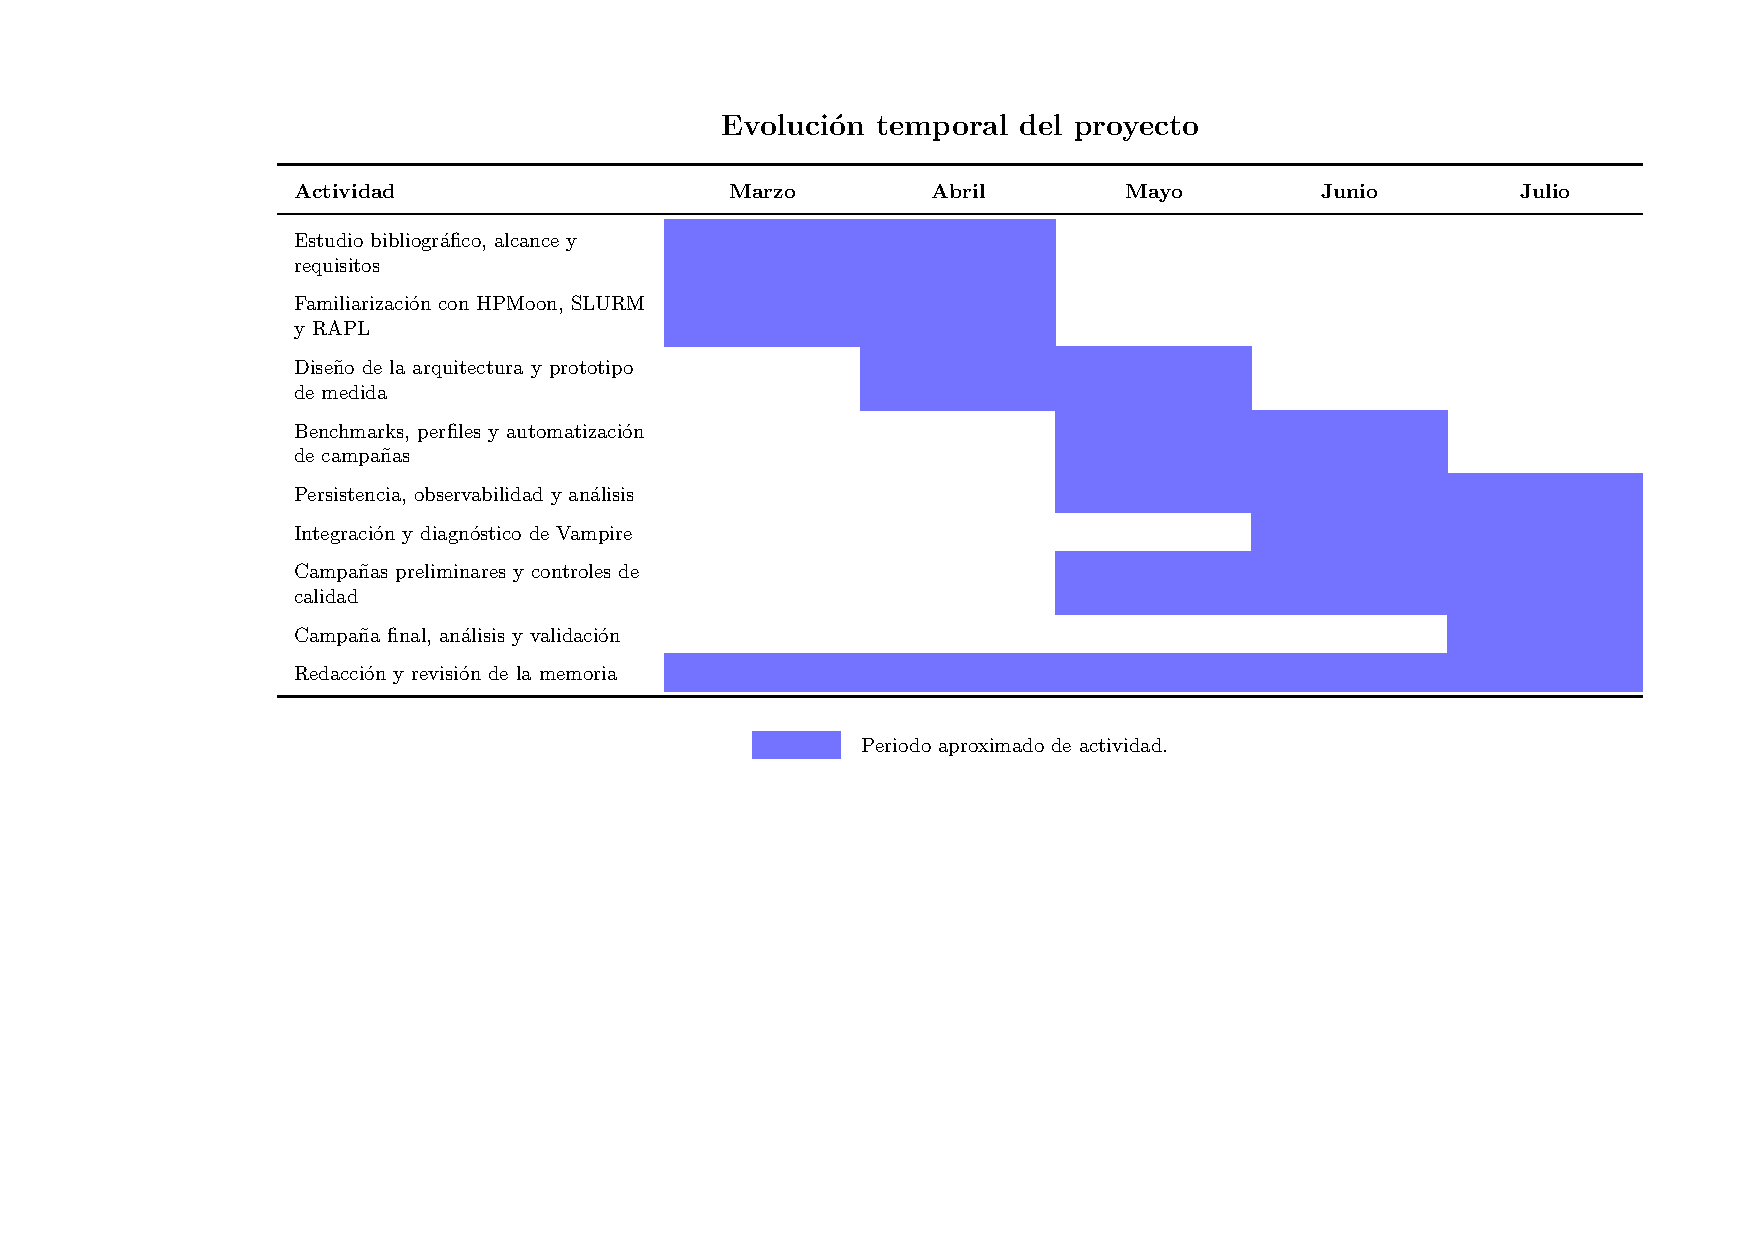
\includegraphics[width=\textwidth]{imagenes/capitulo7/gantt_proyecto.pdf}
    \caption{Evolución temporal aproximada del proyecto entre marzo y julio de 2026.}
    \label{fig:gantt-proyecto}
\end{figure}

El proyecto comenzó con el estudio del entorno HPMoon, el acceso al clúster y la revisión de las herramientas disponibles para la ejecución de trabajos y la medición energética. A partir de esta base se desarrolló un primer prototipo capaz de ejecutar una carga de forma controlada y obtener medidas mediante Intel RAPL. Posteriormente se incorporó la automatización de perfiles, repeticiones y almacenamiento de resultados, lo que permitió pasar de ejecuciones individuales a campañas experimentales completas.

Durante junio se realizaron campañas preliminares orientadas a comprobar el funcionamiento del sistema y a detectar posibles problemas en la adquisición y organización de los datos. Estas ejecuciones se solaparon con el desarrollo del análisis de resultados y con la incorporación de mecanismos de monitorización mediante Prometheus y Grafana. En julio se concentró la integración de la medida externa mediante Vampire, la corrección de incidencias relacionadas con la sincronización y la asociación entre nodo y dispositivo, y la ejecución de la campaña definitiva utilizada en el análisis final.

La documentación se desarrolló de forma paralela al resto del proyecto, recogiendo tanto las decisiones de diseño como la evolución de la implementación, los problemas encontrados y los resultados obtenidos.

\subsection{Principales ajustes durante el desarrollo}
\label{subsec:planificacion-real}

En la tabla~\ref{tab:periodos-desarrollo} se muestra el desarrollo del trabajo 

por meses e hitos funcionales. Los intervalos son aproximados y describen la secuencia y el solapamiento del trabajo, pero no constituyen un registro horario detallado.

\begin{table}[H]
    \centering
    \small
    \caption{Periodos aproximados e hitos principales del desarrollo.}
    \label{tab:periodos-desarrollo}
    \begin{tabular}{p{0.19\textwidth}p{0.30\textwidth}p{0.40\textwidth}}
        \hline
        Periodo aproximado & Trabajo predominante & Resultado principal \\
        \hline
        Marzo--abril & Estudio del problema, delimitación del alcance, familiarización con HPMoon, SLURM y RAPL. & Requisitos y planteamiento inicial de la infraestructura experimental. \\
        Abril--mayo & Diseño de la arquitectura, prototipo de muestreo, cargas controladas y ejecución individual. & Muestreador RAPL, programas de pruebas y primer flujo completo de ejecución. \\
        Mayo--junio & Automatización de matrices, perfiles, persistencia, campañas preliminares y observabilidad. & Configuraciones de campaña, resultados trazables, publicación y paneles de control. \\
        Junio--julio & Integración de Vampire, sincronización, controles de cobertura y diagnóstico de inconsistencias. & Integración externa reforzada, reintentos y herramientas de diagnóstico. \\
        Julio & Verificación de la configuración física, campaña definitiva y análisis. & Paquete validado del 23/07, tablas, figuras y resultados reproducibles. \\
        Marzo--julio & Redacción progresiva y revisión de la memoria. & Memoria LaTeX, anexos y documentación técnica consolidada. \\
        \hline
    \end{tabular}
\end{table}

Las desviaciones más relevantes fueron las siguientes:

\begin{description}
    \item[Acceso al Pushgateway.] La configuración inicial necesitó varios ajustes de dominio, ruta y uso de HTTPS. La consecuencia fue retrasar la estabilización de la observabilidad, sin afectar a los CSV locales. Se mantuvieron los datos almacenados localmente como fuente experimental y la publicación remota como una etapa separada.

    \item[Control de afinidad.] Se diseñaron perfiles utilizando \texttt{numactl}, una herramienta de Linux que permite controlar la asignación de procesos y memoria en sistemas NUMA, y se solicitó la opción \texttt{cpu-bind} de SLURM, utilizada para asociar los procesos a determinadas CPU o núcleos. Sin embargo, durante la campaña SLURM registró que HPMoon no admite esta última opción. Se conservaron el número de tareas y CPU solicitadas, pero se excluyeron del análisis las comparaciones que requerían demostrar una colocación física exacta.

    \item[Cobertura temporal de Vampire.] Algunas capturas preliminares terminaban antes del final del programa de referencia. El procesamiento anterior podía aceptar una ventana parcial, por lo que se reforzó la validación para exigir muestras a ambos lados del intervalo y se añadieron espera posterior y reintentos de descarga. Las ejecuciones incompletas dejaron de producir energía externa aparentemente válida.

    \item[Verificación de la configuración física.] Antes de la campaña definitiva se comprobó la correspondencia entre el nodo de ejecución y el instrumento externo. La batería final se fijó en \texttt{compute-0-4}, asociado a \texttt{hpm4}, y solo las ejecuciones realizadas bajo esta configuración verificada se incorporaron al análisis.

    \item[Publicación y visualización.] La aparición de RAPL sin Vampire en algunos paneles obligó a seguir un mismo \texttt{run\_id} desde el CSV hasta Pushgateway, Prometheus y Grafana. Esto dio lugar a payloads de depuración, consultas separadas por fuente y revisión de variables y etiquetas, evitando atribuir a Grafana fallos producidos en etapas anteriores.

    \item[Selección del dataset.] Las campañas preliminares mezclaban configuraciones y condiciones que dejaron de ser comparables tras las correcciones. En lugar de corregir silenciosamente resultados históricos, se conservó un paquete inmutable de la campaña del 23/07 y se filtró el análisis por su prefijo de ejecución.
\end{description}

Estas desviaciones ampliaron el esfuerzo de diagnóstico y obligaron a repetir campañas, pero también produjeron controles que forman parte del resultado: validación de ventanas, políticas de fallo, reintentos, cargas de trabajo auditables y análisis reproducible.

\section{Recursos utilizados}
\label{sec:planificacion-recursos}

\subsection{Recursos hardware e infraestructura}
\label{subsec:recursos-hardware}

La tabla~\ref{tab:recursos-hardware} resume los recursos utilizados. La caracterización técnica del nodo se detalla en el capítulo~\ref{chap:entorno}.

\begin{table}[htbp]
    \centering
    \small
    \caption{Recursos hardware e infraestructuras utilizados.}
    \label{tab:recursos-hardware}
    \begin{tabular}{p{0.20\textwidth}p{0.22\textwidth}p{0.43\textwidth}}
        \hline
        Recurso & Tipo & Uso en el proyecto \\
        \hline
        HPMoon &
        Clúster de computadores &
        Ejecución de trabajos mediante SLURM y acceso a los recursos de cómputo necesarios para las campañas experimentales. \\

        \texttt{compute-0-4} &
        Nodo de cómputo &
        Nodo utilizado para la campaña definitiva, sobre el que se ejecutan los programas de prueba y se obtienen las medidas internas mediante RAPL. \\

        Vampire \texttt{hpm4} &
        Vatímetro externo &
        Medición externa de la potencia y la energía asociadas al nodo \texttt{compute-0-4}. \\

        VPS de observabilidad &
        Servidor virtual &
        Alojamiento mediante Docker de HAProxy, Pushgateway, Prometheus y Grafana para la publicación, recopilación y visualización de métricas. Su coste imputable durante los cinco meses del proyecto asciende a 60~EUR. \\

        Equipo de desarrollo y red &
        Infraestructura de desarrollo y comunicaciones &
        Edición del proyecto, acceso al clúster, realización de pruebas locales y redacción de la memoria. No se registró el detalle necesario para imputar su amortización. \\
        \hline
    \end{tabular}
\end{table}

\subsection{Recursos software}
\label{subsec:recursos-software}

El software desarrollado incluye: el muestreador RAPL, los programas de prueba, el orquestador de ejecuciones, el generador de matrices, la construcción de métricas y los scripts de diagnóstico y análisis. Además, el sistema se integra con el dispositivo externo Vampire para obtener las medidas eléctricas del nodo. Sobre estos componentes se utilizaron las herramientas externas de la tabla~\ref{tab:recursos-software}.

\begin{table}[htbp]
    \centering
    \small
    \caption{Principales recursos software externos.}
    \label{tab:recursos-software}
    \begin{tabular}{p{0.28\textwidth}p{0.61\textwidth}}
        \hline
        Recurso & Finalidad \\
        \hline
        Linux y \emph{powercap} & Entorno de ejecución y acceso a \texttt{energy\_uj} para el muestreo RAPL. \\
        SLURM y \texttt{sacct} & Reserva, ejecución y consulta del estado final de los trabajos. \\
        Python 3 & Orquestación, adquisición, persistencia, diagnóstico, pruebas y análisis. \\
        C y GCC & Implementación y compilación de las cargas utilizadas en la campaña final. \\
        \texttt{numactl} y \texttt{taskset} & Solicitud e inspección de colocación de CPU y memoria en campañas exploratorias. \\
        Cliente Vampire e InfluxDB & Inicio, parada y descarga de las muestras externas. \\
        Docker y Docker Compose & Despliegue aislado y reproducible de los servicios de observabilidad en el VPS. \\
        HAProxy, Certbot y Let's Encrypt & Enrutamiento por subrutas, terminación HTTPS y gestión de certificados del dominio público. \\
        Pushgateway, Prometheus y Grafana & Recepción, recopilación, consulta y visualización de agregados. \\
        Bibliotecas Python & Procesamiento y representación mediante Pandas, Pillow, Matplotlib y Seaborn, además de dependencias del cliente Vampire. \\
        \texttt{unittest} & Pruebas locales de monitorización, selección de nodo e integración externa simulada. \\
        Git y LaTeX & Control de versiones, trazabilidad del desarrollo y elaboración de la memoria. \\
        \hline
    \end{tabular}
\end{table}

El código fuente y las configuraciones necesarias para reproducir el sistema se encuentran disponibles en el repositorio indicado en el Anexo~\ref{anexo:scripts}.

Los nodos de HPMoon proporcionan el entorno Linux utilizado para ejecutar las campañas. Por otra parte, el sistema de observabilidad se desplegó en un VPS con Ubuntu 24.04 mediante Docker y Docker Compose. Estos últimos permiten mantener separados HAProxy, Pushgateway, Prometheus y Grafana, así como conservar su configuración mediante volúmenes y directorios enlazados.

\section{Recursos humanos}
\label{sec:planificacion-esfuerzo}

Una única persona desempeñó las tareas de análisis, diseño, desarrollo, integración, experimentación, análisis de datos y documentación. Dado que no se mantuvo un registro horario detallado, el esfuerzo se ha estimado retrospectivamente tomando como referencia la carga académica del Proyecto Fin de Grado. La asignatura tiene asignados 12 créditos ECTS \parencite{ugrGuiaPfg2025}, y cada crédito representa entre 25 y 30 horas de trabajo del estudiante \parencite{realDecreto1125_2003}. Para obtener una estimación conservadora se adopta el límite inferior, correspondiente a 300 horas de dedicación. La Tabla~\ref{tab:esfuerzo-fases} distribuye este esfuerzo entre las principales fases del proyecto.

\begin{table}[htbp]
    \centering
    \caption{Estimación del esfuerzo dedicado a las distintas fases del proyecto.}
    \label{tab:esfuerzo-fases}
    \begin{tabular}{p{0.64\textwidth}r}
        \hline
        \textbf{Fase} & \textbf{Horas estimadas} \\
        \hline
        Estudio del entorno y antecedentes & 40 \\
        Diseño e implementación del sistema & 90 \\
        Integración de observabilidad y Vampire & 50 \\
        Pruebas, diagnóstico y correcciones & 45 \\
        Campañas y análisis de datos & 35 \\
        Documentación y memoria & 40 \\
        \hline
        \textbf{Total} & \textbf{300} \\
        \hline
    \end{tabular}
\end{table}

\section{Estimación de costes}
\label{sec:planificacion-costes}

La estimación económica distingue entre la valoración del trabajo realizado y los costes directos de infraestructura, energía y licencias. Las cantidades presentadas no representan pagos efectuados al autor, sino una aproximación al coste que tendría desarrollar el proyecto utilizando una referencia salarial profesional y los recursos empleados. Las hipótesis aplicadas a cada partida se indican explícitamente para evitar atribuir una precisión superior a la disponible.

\subsection{Personal}

El esfuerzo se valora utilizando como referencia el Área 3 del XIX Convenio colectivo estatal de empresas de consultoría, tecnologías de la información y estudios de mercado, que comprende actividades de desarrollo de software, programación y explotación de sistemas. Dentro de esta área se adopta el grupo C, nivel 3, por corresponder a un perfil técnico con poca experiencia profesional y autonomía en la ejecución de tareas \parencite{convenioConsultoria2025}.

La tabla salarial actualizada para 2026 establece para esta categoría una retribución anual de 24.105,37~EUR \parencite{tablasConsultoria2026}. Considerando la jornada máxima de 1.800 horas anuales establecida por el convenio, la tarifa horaria de referencia es:

\begin{equation}
    t_{\mathrm{personal}}=
    \frac{24\,105{,}37}{1\,800}
    =13{,}39~\mathrm{EUR/h}.
    \label{eq:tarifa-personal}
\end{equation}

El coste de personal se obtiene multiplicando las 300 horas estimadas por la tarifa horaria:

\begin{equation}
    C_{\mathrm{personal}}=
    300\times13{,}39
    =4\,017{,}00~\mathrm{EUR}.
    \label{eq:coste-personal}
\end{equation}

Esta cantidad representa una valoración económica del trabajo realizado a partir de una referencia profesional pública. No corresponde a una remuneración percibida por el autor ni incorpora costes empresariales indirectos.

\subsection{Infraestructura y energía}

No resulta adecuado imputar a este trabajo el coste de adquisición de HPMoon, ya que se trata de una infraestructura previamente disponible en la Universidad y no se dispone de una tarifa interna por hora de nodo. Por este motivo, su coste directo se considera nulo, aunque su utilización constituye un recurso necesario para el desarrollo del proyecto.

El sistema de observabilidad se desplegó en un VPS contratado por 12~EUR mensuales. Dado que la planificación comprende los cinco meses transcurridos entre marzo y julio, su coste imputable es:

\begin{equation}
    C_{\mathrm{VPS}} =
    12 \times 5 =
    60{,}00~\mathrm{EUR}.
    \label{eq:coste-vps}
\end{equation}

El dominio utilizado para acceder a los servicios tiene un precio anual de 6~EUR. La imputación proporcional correspondiente al mismo periodo es:

\begin{equation}
    C_{\mathrm{dominio}} =
    6 \times \frac{5}{12} =
    2{,}50~\mathrm{EUR}.
    \label{eq:coste-dominio}
\end{equation}

No se imputa un coste adicional al equipo de desarrollo, puesto que era un recurso disponible previamente y no se adquirió específicamente para el proyecto.

La energía externa acumulada durante las ventanas de prueba de la campaña final es 1.354.943~J, equivalentes a 0,376~kWh. Esta cifra no comprende el desarrollo, las campañas preliminares, los tiempos en cola, la captura anterior y posterior a cada programa de referencia ni el resto de la infraestructura. Sirve únicamente para cuantificar la energía registrada durante las ventanas de ejecución de la campaña final.

La conversión de julios a kilovatios-hora se realiza mediante:

\begin{equation}
    E_{\mathrm{kWh}} =
    \frac{E_{\mathrm{Vampire}}}{3{,}6\times10^6},
    \qquad
    1~\mathrm{kWh}=3{,}6\times10^6~\mathrm{J}.
    \label{eq:conversion-energia}
\end{equation}

Aplicando esta expresión a la energía acumulada de la campaña:

\[
    E_{\mathrm{kWh}} =
    \frac{1\,354\,943}{3{,}6\times10^6}
    \approx 0{,}376~\mathrm{kWh}.
\]

Para valorar esta energía se adopta como referencia el precio medio de la electricidad para consumidores domésticos en España durante el segundo semestre de 2025, correspondiente a 0,2669~EUR/kWh, incluidos impuestos y gravámenes \parencite{eurostatElectricidad2025}. Se utiliza una tarifa doméstica de referencia, y no el precio específico que pudiera pagar la Universidad, porque el objetivo es proporcionar una estimación económica reproducible basada en un valor público.

\begin{equation}
    C_{\mathrm{energia}} =
    0{,}376 \times 0{,}2669
    \approx 0{,}10~\mathrm{EUR}.
    \label{eq:coste-energia}
\end{equation}

Esta partida corresponde exclusivamente a la energía externa registrada durante las ventanas de ejecución de la campaña final. No incluye las campañas preliminares, el consumo del VPS, el equipo de desarrollo ni el funcionamiento habitual de HPMoon. No se utiliza la energía RAPL para valorar la electricidad adquirida porque representa únicamente los dominios internos \texttt{package}.

\subsection{Software y coste total}

Las herramientas principales son software libre, de código abierto o servicios ya disponibles en la infraestructura universitaria, por lo que no generaron costes directos de licencias imputables al proyecto. Un coste de licencia igual a cero no implica coste de integración nulo: la instalación, configuración, diagnóstico y mantenimiento se incluyen en el apartado de recursos humanos.

La tabla~\ref{tab:coste-total} resume las partidas consideradas. El coste de personal constituye la mayor parte del presupuesto, mientras que los costes directos de infraestructura son reducidos debido al uso de recursos previamente disponibles y herramientas sin coste de licencia.

\begin{table}[htbp]
    \centering
    \caption{Valoración económica y costes directos estimados del proyecto.}
    \label{tab:coste-total}
    \begin{tabular}{p{0.59\textwidth}r}
        \hline
        Concepto & Coste estimado (EUR) \\
        \hline
        Personal & 4.017,00 \\
        Uso de HPMoon (coste directo imputado) & 0,00 \\
        VPS durante cinco meses & 60,00 \\
        Dominio durante cinco meses & 2,50 \\
        Energía registrada en la campaña final & 0,10 \\
        Equipo de desarrollo (coste directo imputado) & 0,00 \\
        Software y licencias directas & 0,00 \\
        \hline
        \textbf{Total} & \textbf{4.079,60} \\
        \hline
    \end{tabular}
\end{table}

El total estimado asciende a 4.079,60~EUR. Esta cifra representa una valoración económica del desarrollo y de los costes directos documentados, no el desembolso efectivo realizado durante el TFG.

\section{Gestión de riesgos}
\label{sec:planificacion-riesgos}

La gestión de riesgos se integró en el flujo mediante validaciones, persistencia por ejecución y políticas de fallo. La probabilidad y el impacto de la tabla~\ref{tab:riesgos-proyecto} se estimaron cualitativamente al cierre del proyecto; no proceden de un análisis probabilístico formal.

\begingroup
\small
\setlength{\tabcolsep}{4pt}
\renewcommand{\arraystretch}{1.16}
\begin{longtable}{|
    >{\raggedright\arraybackslash}p{0.05\textwidth}|
    >{\raggedright\arraybackslash}p{0.17\textwidth}|
    >{\raggedright\arraybackslash}p{0.165\textwidth}|
    >{\raggedright\arraybackslash}p{0.315\textwidth}|
    >{\raggedright\arraybackslash}p{0.155\textwidth}|}
    \caption{Principales riesgos y respuesta adoptada.}
    \label{tab:riesgos-proyecto} \\
    \hline
    \rowcolor[gray]{0.90}
    \textbf{ID} & \textbf{Riesgo} & \textbf{P/I} & \textbf{Prevención, mitigación y contingencia} & \textbf{Estado final} \\
    \hline
    \endfirsthead
    \multicolumn{5}{c}{\tablename\ \thetable\ (continuación)} \\
    \hline
    \rowcolor[gray]{0.90}
    \textbf{ID} & \textbf{Riesgo} & \textbf{P/I} & \textbf{Prevención, mitigación y contingencia} & \textbf{Estado final} \\
    \hline
    \endhead
    R1 & Nodo no disponible o trabajo interrumpido & Media/alta & Ejecución mediante SLURM, consulta de \texttt{sacct} y estado persistido; repetir solo ejecuciones afectadas. & Gestionado. \\
    \hline
    R2 & Permisos insuficientes para RAPL o recursos & Media/alta & Validación previa del entorno y ejecución del muestreador dentro del nodo asignado. & Gestionado en el nodo final. \\
    \hline
    R3 & Afinidad solicitada no aplicada & Media/media & Conservar comandos y logs; limitar las conclusiones a CPU asignadas y excluir comparaciones físicas no verificadas. & Limitación abierta. \\
    \hline
    R4 & Captura Vampire incompleta & Alta/alta & Validar cobertura, ampliar espera, reintentar descarga y no publicar energía falsa cuando falla; repetir la prueba. & Corregido para la campaña final. \\
    \hline
    R5 & Asociación nodo--medidor no verificada & Media/alta & Mapa explícito nodo--dispositivo y comprobación previa antes de iniciar la campaña definitiva. & Verificada. \\
    \hline
    R6 & Fallo de Pushgateway o del VPS & Media/media & Reintentos, timeout, registro del error y conservación local de CSV y JSON; republicar o consultar localmente. & Mitigado. \\
    \hline
    R7 & Pérdida o mezcla de resultados & Media/alta & \texttt{run\_id}, directorios por campaña, raw JSON, logs y paquetes inmutables; copia antes de retirar grupos antiguos. & Mitigado. \\
    \hline
    R8 & Ruido o ejecuciones anómalas & Media/media & Reserva exclusiva, repeticiones, controles de calidad y coeficientes de variación; excluir y repetir casos no válidos. & Evaluado en la campaña final. \\
    \hline
    R9 & Error de procesamiento o unidades & Media/alta & Pruebas automáticas y recálculo independiente desde los CSV de ambas fuentes. & Verificado en 61 ejecuciones. \\
    \hline
    R10 & Tiempo insuficiente para repetir & Media/alta & Campañas diagnósticas cortas, ejecución secuencial y validación previa antes de lanzar la batería completa. & Mitigado. \\
    \hline
\end{longtable}
\endgroup

\section{Sostenibilidad del proyecto}
\label{sec:planificacion-sostenibilidad}

\subsection{Impacto medioambiental}

El proyecto no implementa directamente una política de reducción del consumo, pero proporciona la infraestructura y la información necesarias para estudiar el comportamiento energético del clúster y fundamentar futuras decisiones de optimización. La comparación entre rendimiento y consumo permite identificar configuraciones en las que un aumento de los recursos asignados no se traduce en una mejora proporcional del rendimiento, pero sí en un mayor consumo energético.

La validación previa también evita repetir campañas completas por errores detectables de configuración, sincronización o publicación. Este efecto reduce potencialmente ejecuciones inútiles, aunque no se ha cuantificado una reducción de consumo ni de emisiones atribuible al TFG.

\subsection{Dimensión económica}

La automatización reduce trabajo manual y permite reutilizar campañas, diagnósticos y análisis. Las herramientas externas empleadas no introducen costes directos de licencia documentados y aprovechan infraestructura académica existente. No obstante, el tiempo de integración y mantenimiento sigue constituyendo un coste profesional, como refleja la estimación del coste de personal.

\subsection{Dimensión técnica}

La arquitectura modular del sistema, junto con el uso de formatos abiertos como CSV y JSON, la conservación de las muestras originales y la documentación del proceso, facilita su mantenimiento y reutilización. La posibilidad de incorporar nuevas cargas, perfiles, nodos de cómputo o fuentes de medida sin reconstruir completamente la plataforma permite ampliar el sistema progresivamente y aprovechar el desarrollo realizado en futuras campañas sobre el clúster de pruebas HPMoon.

Desde esta perspectiva, la sostenibilidad técnica se relaciona con la capacidad de mantener, reutilizar y ampliar la infraestructura desarrollada a lo largo del tiempo. Además, disponer de medidas reproducibles de rendimiento y consumo proporciona una base para estudiar posteriormente configuraciones más eficientes. Las posibles mejoras ambientales o económicas dependerán de las decisiones de optimización que se adopten a partir de estos datos y de su validación mediante nuevas campañas.

\chapter{Conclusiones y trabajos futuros}
\label{chap:conclusiones}

\section{Conclusiones}
\label{sec:conclusiones}

El objetivo de este Trabajo Fin de Grado ha sido diseñar, desarrollar y validar un sistema que permita estudiar el consumo energético asociado a la ejecución de cargas de trabajo sobre un clúster de computadores. El resultado obtenido va más allá de la adquisición puntual de medidas energéticas: se ha construido una infraestructura experimental capaz de coordinar un conjunto de ejecuciones bajo diferentes configuraciones, la ejecución de trabajos mediante SLURM, la adquisición de medidas de energía con medidores internos y externos, el almacenamiento de los resultados y su posterior análisis.

Este trabajo ha permitido transformar una configuración experimental en un conjunto de ejecuciones identificadas y trazables. Cada prueba conserva no solo sus medidas finales, sino también las muestras originales, los parámetros utilizados, los metadatos de cada ejecución y la información necesaria para relacionar los distintos parámetros del experimento. De este modo, los resultados pueden revisarse y recalcularse posteriormente sin depender de una visualización en tiempo real o de un único fichero agregado.

La validación del sistema se ha realizado mediante 61 ejecuciones válidas sobre el nodo \texttt{compute-0-4} de un clúster de computadores. Para ello, se han utilizado tres tipos de cargas: un programa Idle como referencia basal, un conjunto de programas de prueba orientados poner a prueba el ancho de banda de la memoria, utilizando STREAM y un programa de cálculo intensivo, con el benchmark DGEMM. Para las dos cargas activas se estudiaron perfiles con 1, 2, 4, 6, 8 y 12 procesos, realizando cinco repeticiones por configuración y manteniendo una duración objetivo de 120~s.

Los resultados obtenidos muestran que el sistema es capaz de distinguir comportamientos energéticos diferentes en función del tipo de carga y de los recursos utilizados. Idle presenta, como era esperable, los niveles de potencia más bajos, mientras que STREAM y DGEMM incrementan el consumo energético al aumentar el número de procesos. Sin embargo, este incremento no se traduce de la misma manera en rendimiento para ambas cargas.

En STREAM, el mayor rendimiento medio se alcanza con cuatro procesos y la incorporación de recursos adicionales no produce una mejora proporcional. Esto provoca que, a partir de determinados perfiles, el consumo continúe aumentando sin que exista un incremento equivalente del trabajo realizado. DGEMM presenta un comportamiento diferente, ya que el rendimiento continúa aumentando hasta doce procesos y la relación entre el trabajo realizado y la energía consumida evoluciona de forma más favorable.

Este comportamiento pone de manifiesto una de las ideas principales del trabajo: \textbf{utilizar más recursos de cómputo no implica necesariamente obtener una mejora proporcional del rendimiento ni de la eficiencia energética}. La configuración más adecuada depende principalmente del tipo de carga y del objetivo perseguido. Analizar conjuntamente el rendimiento y el consumo permite identificar configuraciones en las que aumentar los recursos aporta poca mejora de rendimiento, pero sí incrementa el consumo energético.

La estabilidad de las medidas se ha evaluado realizando cinco repeticiones  para cada configuración activa. La dispersión observada es reducida en comparación con las diferencias existentes entre perfiles. El coeficiente de variación máximo de la energía fue del 0,65~\% para las medidas obtenidas con RAPL y del 1,04~\% para los datos obtenidos con Vampire. El coeficiente de variación del rendimiento de STREAM es inferior al 0,55~\%, mientras que el DGEMM es del orden del 5,43~\%, para cuatro procesos. La baja dispersión observada entre repeticiones de una misma configuración indica que el procedimiento produce resultados estables bajo condiciones equivalentes, lo que respalda su repetibilidad dentro del entorno estudiado.

La utilización de dos medidores, Intel RAPL y Vampire, aporta diferente información sobre el comportamiento energético del sistema. RAPL proporciona información correspondiente a determinados componentes del procesador (\texttt{package}), mientras que Vampire registra el consumo eléctrico global del nodo completo. 

Por tanto, la principal aportación experimental no consiste en determinar unos  valores de consumo, sino en desarrollar una infraestructura que permite medir el consumo energético de programas de prueba con diferentes configuraciones de forma automatizada, trazable y repetible, obteniendo información suficientemente estable para estudiar diferencias entre cargas y configuraciones.

En un contexto en el que las necesidades de cómputo continúan aumentando, el rendimiento no puede analizarse de forma completamente independiente del consumo energético necesario para obtenerlo. El sistema desarrollado no reduce por sí mismo el consumo del clúster, pero permite cuantificar la relación entre los recursos utilizados, el rendimiento obtenido y la energía consumida. Esta información constituye una base para identificar configuraciones poco eficientes y, en futuros trabajos, plantear estrategias de utilización y asignación de recursos que tengan en cuenta tanto el rendimiento como el consumo energético.

\section{Cumplimiento de los objetivos}
\label{sec:objetivos-cumplimiento}

Los objetivos planteados al inicio del trabajo se consideran alcanzados dentro del alcance experimental definido. El objetivo general, consistente en diseñar, implementar y validar un sistema para medir y analizar el consumo energético asociado a las CPU del clúster HPMoon durante la ejecución de cargas controladas, se ha materializado en una infraestructura funcional y validada mediante una campaña experimental completa.

La Tabla~\ref{tab:cumplimiento-objetivos} relaciona los principales objetivos específicos con los resultados alcanzados.

\begingroup
\small
\setlength{\tabcolsep}{4pt}
\renewcommand{\arraystretch}{1.16}

\begin{longtable}{|p{0.27\textwidth}|p{0.535\textwidth}|p{0.12\textwidth}|}
    \caption{Cumplimiento de los objetivos específicos del proyecto.}
    \label{tab:cumplimiento-objetivos}\\
    \hline
    \textbf{Objetivo} & \textbf{Resultado alcanzado} & \textbf{Estado} \\
    \hline
    \endfirsthead

    \multicolumn{3}{c}{\tablename\ \thetable{} (continuación)}\\
    \hline
    \textbf{Objetivo} & \textbf{Resultado alcanzado} & \textbf{Estado} \\
    \hline
    \endhead

    Caracterizar el entorno de ejecución y los mecanismos de medida. &
    Se estudiaron HPMoon, SLURM, la topología del nodo y las interfaces utilizadas para la medición mediante RAPL y Vampire. &
    Cumplido \\
    \hline

    Definir una arquitectura modular para el sistema. &
    La solución separa la configuración de campañas, la ejecución, la adquisición de medidas, el almacenamiento, la publicación y el análisis de resultados. &
    Cumplido \\
    \hline

    Automatizar combinaciones de carga, recursos y repeticiones. &
    La plataforma genera y ejecuta las distintas configuraciones experimentales a partir de la definición de cada campaña. &
    Cumplido \\
    \hline

    Integrar la adquisición energética mediante Intel RAPL. &
    Se realiza un muestreo periódico de los dominios \texttt{package}, conservando tanto las muestras como las métricas agregadas de cada ejecución. &
    Cumplido \\
    \hline

    Integrar la medida externa mediante Vampire. &
    La captura externa se coordina con la ejecución del programa de referencia y se comprueba que cubra correctamente la ventana temporal analizada. &
    Cumplido \\
    \hline

    Mantener la trazabilidad de las ejecuciones. &
    Cada ejecución conserva un identificador \texttt{run\_id} que permite relacionar configuración, muestras, resultados, estados y metadatos. &
    Cumplido \\
    \hline

    Incorporar monitorización y visualización. &
    Los agregados pueden publicarse mediante Pushgateway, recopilarse con Prometheus y visualizarse en Grafana, manteniendo los datos experimentales originales como fuente del análisis. &
    Cumplido \\
    \hline

    Diseñar y ejecutar una campaña experimental. &
    Se completó una campaña formada por 61 ejecuciones válidas con tres tipos de carga y seis perfiles de ejecución para las cargas activas. &
    Cumplido \\
    \hline

    Desarrollar un procedimiento de análisis reproducible. &
    Las métricas pueden recalcularse a partir de las muestras originales y se aplican controles de calidad antes de incorporar una ejecución al conjunto analizado. &
    Cumplido \\
    \hline

\end{longtable}
\endgroup

\section{Aportaciones del trabajo}
\label{sec:aportaciones}

Una de las principales aportaciones del trabajo es la integración de componentes y tecnologías diferentes dentro de un único flujo experimental. La solución desarrollada coordina el gestor de trabajos del clúster, programas de referencia, medidores internos (Intel RAPL) y externos (Vampire), el almacenamiento de resultados y las herramientas de monitorización. Esta integración permite que una campaña completa pueda ejecutarse siguiendo un procedimiento homogéneo y reduciendo la intervención manual.

Otra aportación relevante es la trazabilidad de los experimentos. Cada ejecución conserva su configuración, sus muestras de energía, los resultados del programa de referencia y los metadatos necesarios para conocer las condiciones en las que se realizó. La utilización de un identificador común permite relacionar las distintas fuentes de información y reconstruir posteriormente los resultados sin modificar los datos originales.

El trabajo también aporta un procedimiento de validación que no se limita a comprobar que una ejecución haya finalizado correctamente. Antes de incorporar una prueba al conjunto de resultados se consideran aspectos como el estado del trabajo, la existencia de los ficheros esperados, la cobertura temporal de las medidas, el número de muestras y la coherencia de los valores obtenidos. La aplicación de estos controles permite detectar problemas durante las campañas preliminares, corregir el sistema y repetir las pruebas con una configuración adecuada en lugar de modificar retrospectivamente los datos obtenidos.

Desde el punto de vista experimental, la infraestructura permite relacionar el consumo energético con el comportamiento de distintos tipos de carga. Los resultados obtenidos al ejecutar STREAM y DGEMM muestran que una misma ampliación de recursos puede tener efectos diferentes sobre el rendimiento y la eficiencia dependiendo del patrón de trabajo. Esta capacidad convierte la plataforma en una base útil para estudiar configuraciones de ejecución y no únicamente para registrar valores de potencia o energía.

Además, el desarrollo combina conocimientos pertenecientes a distintas áreas de la Ingeniería Informática. El trabajo requiere abordar aspectos relacionados con sistemas operativos, administración de clústeres, arquitectura de computadores, programación, automatización, monitorización, tratamiento de datos y metodología experimental. La integración de estas áreas ha sido necesaria para obtener una solución funcional sobre una infraestructura real y no únicamente sobre un entorno de laboratorio controlado.

Por último, la arquitectura desarrollada permite ampliar el sistema sin modificar su planteamiento fundamental. Nuevas cargas, perfiles de ejecución o nodos pueden incorporarse mediante nuevas campañas, mientras que los mecanismos de adquisición y almacenamiento pueden seguir utilizándose. Esta capacidad de extensión resulta especialmente relevante para continuar estudiando el compromiso entre rendimiento y consumo energético en HPMoon.

\section{Limitaciones}
\label{sec:limitaciones-conclusiones}

Los resultados obtenidos deben interpretarse dentro del alcance de la campaña realizada. La evaluación se ha llevado a cabo sobre el nodo \texttt{compute-0-4} del clúster HPMOON, equipado con dos procesadores Intel Xeon Silver 4214. Por tanto, las tendencias observadas caracterizan esta configuración y no pueden extrapolarse directamente a otros tipos de nodos, procesadores, arquitecturas o clústeres.

Las cargas utilizadas son sintéticas y representan tres situaciones concretas: baja actividad mediante Idle, presión sobre el subsistema de memoria mediante una carga basada en STREAM y cálculo intensivo con DGEMM. Aunque esta selección permite observar comportamientos diferenciados, no reproduce toda la variedad de aplicaciones que pueden ejecutarse en un entorno HPC.

La campaña utiliza seis perfiles de ejecución para las cargas activas y no estudia de forma específica los efectos sobre una arquitectura NUMA, sisteas multihilo simultáneo (SMT), frecuencia del procesador o diferentes estrategias de afinidad. Además, aunque se solicita el número de procesos y recursos necesarios para cada ejecución, no se pudo verificar de forma exacta en qué núcleos físicos del nodo se ejecutó cada proceso.

El programa Idle se ejecuta una única vez al utilizarse como referencia basal. En consecuencia, esta prueba permite disponer de un valor de referencia, pero no estudiar su variabilidad entre repeticiones al mismo nivel que STREAM y DGEMM.

Otra limitación deriva del diseño temporal de las cargas. STREAM y DGEMM repiten sus operaciones durante una ventana de duración aproximadamente constante. Este planteamiento facilita la obtención de medidas energéticas estables, pero hace que cada configuración pueda completar una cantidad diferente de trabajo durante el mismo intervalo. Por este motivo, métricas como el producto energía--retardo no pueden interpretarse de la misma forma que en una campaña en la que todas las configuraciones resuelvan exactamente el mismo problema.

Los dos medidores utilizados miden consumos diferentes. Intel RAPL proporciona información correspondiente a componentes del procesador (\texttt{package}) concretos, mientras que Vampire mide el consumo global del nodo. La diferencia entre ambas medidas no puede utilizarse para atribuir directamente el consumo a componentes concretos. Además, Vampire utiliza una frecuencia de muestreo de 5~s, frente al de 1~s utilizado por RAPL, por lo que los valores máximos obtenidos por ambas fuentes no son directamente comparables muestra a muestra.

Finalmente, la coherencia observada entre las medidas y su repetibilidad no constituyen una calibración metrológica absoluta de los instrumentos. El trabajo valida el funcionamiento de la infraestructura y la consistencia de los resultados dentro de las condiciones estudiadas, pero una caracterización de precisión absoluta requeriría instrumentación y procedimientos específicos de calibración.

\section{Trabajos futuros}
\label{sec:trabajo-futuro}

El sistema desarrollado constituye una base sobre la que pueden plantearse nuevas líneas de experimentación. Una primera ampliación consiste en aumentar la variedad de entornos evaluados. La ejecución de campañas equivalentes sobre otros nodos de HPMoon permitiría estudiar si las tendencias observadas se mantienen entre diferentes generaciones de procesadores y configuraciones hardware.

También resulta de interés ampliar el conjunto de cargas utilizadas. La incorporación de aplicaciones científicas reales permitiría complementar los programas sintéticos y estudiar escenarios más próximos al uso habitual de un clúster HPC. Del mismo modo, aumentar el número de repeticiones de Idle permitiría caracterizar con mayor precisión el consumo basal del nodo.

Otra línea de trabajo consiste en modificar el planteamiento temporal de los programas de referencia. Una campaña en la que todas las configuraciones deban completar una cantidad fija de trabajo permitiría estudiar directamente el tiempo necesario para resolver el mismo problema y analizar métricas como el \emph{speedup}, la energía total o el producto energía--retardo. Este enfoque complementaría la campaña de duración controlada utilizada en este trabajo.

El estudio de la CPU puede ampliarse introduciendo de forma controlada nuevas variables experimentales. Entre ellas se encuentran el uso de SMT, diferentes distribuciones NUMA, políticas de frecuencia o límites de potencia. La incorporación de contadores hardware mediante herramientas como \texttt{perf} permitiría además relacionar el consumo energético con variables como el número de instrucciones ejecutadas, los ciclos de procesador o determinados eventos de memoria y caché.

En relación con la medición energética, una futura ampliación podría caracterizar con mayor detalle la relación entre los dominios observados mediante RAPL y el consumo global registrado por Vampire. También sería de interés analizar de forma específica el consumo basal del nodo y estudiar cómo cambia la proporción entre ambas medidas para distintos tipos de carga. Si se dispusiera de instrumentación de referencia adecuada, podría realizarse además una calibración independiente de la cadena de medida.

Desde el punto de vista del software, el sistema puede evolucionar incorporando nuevos mecanismos de automatización. Entre las posibles mejoras se encuentran el registro automático de la asignación efectiva de CPU, la agregación directa del trabajo producido por todos los procesos, la detección automática de ejecuciones anómalas y la generación de informes comparativos entre campañas.

La acumulación de resultados a lo largo de múltiples campañas permitiría dar un paso adicional. En lugar de limitarse a describir el comportamiento energético de una configuración, los datos podrían utilizarse para identificar qué cantidad de recursos resulta más adecuada para una determinada clase de carga. Por ejemplo, sería posible detectar situaciones en las que aumentar el número de procesos incrementa el consumo sin producir una mejora significativa del rendimiento.

A partir de esta información podría desarrollarse una capa de recomendación capaz de seleccionar configuraciones en función de diferentes objetivos, como minimizar la energía consumida, limitar la potencia utilizada o alcanzar un determinado nivel de rendimiento. De esta manera, la infraestructura evolucionaría desde un sistema de medida y análisis hacia una herramienta de apoyo a la toma de decisiones.

A más largo plazo, este enfoque podría extenderse al propio planificador del clúster. La información obtenida sobre rendimiento y consumo podría servir como base para estudiar estrategias de planificación conscientes de la energía, en las que la asignación de recursos no dependiera únicamente de su disponibilidad, sino también del coste energético asociado a las distintas configuraciones.

También podría explorarse la utilización de técnicas estadísticas o modelos predictivos capaces de estimar el consumo esperado de una ejecución a partir de sus características y de los recursos asignados. Estas líneas requerirían campañas experimentales más amplias, pero representan una evolución natural de la infraestructura construida en este trabajo.

En todos estos casos, el punto de partida continúa siendo el mismo: disponer de datos energéticos fiables, contextualizados y reproducibles. Sin una infraestructura que permita medir de forma consistente, cualquier estrategia posterior de optimización o recomendación carecería de una base experimental adecuada.

% Anexos
\appendix

\chapter{Entorno y requisitos de ejecución}
\label{anexo:entorno}

El sistema requiere Python 3, un compilador C, acceso a SLURM y permisos de lectura sobre la interfaz RAPL del nodo. Para utilizar la medición externa se requiere además acceso al cliente \texttt{vampire.py}, facilitado por la Universidad de Granada y no distribuido en el repositorio, y al servicio del que este obtiene las muestras. Los benchmarks se compilan mediante el \texttt{Makefile} del repositorio y las campañas se ejecutan desde el directorio raíz. La comprobación local, que no se comunica con el clúster ni con los servicios remotos, se realiza con la siguiente orden:

\begin{lstlisting}[style=Consola]
python3 -m unittest discover -s tests
python3 scripts/validate_campaign_singlethread.py \
  campaigns/hpc-tfg-main-campaign.json
\end{lstlisting}

La campaña se lanza con la siguiente orden:

\begin{lstlisting}[style=Consola]
python3 run_matrix.py \
  --config campaigns/hpc-tfg-main-campaign.json
\end{lstlisting}

Las URL y posibles credenciales del sistema remoto se proporcionan mediante variables de entorno y no se almacenan en la memoria ni en los resultados publicados. La configuración permite comprobar localmente el procesamiento, las etiquetas y el payload sin realizar conexiones remotas.

La campaña final se ejecutó en \texttt{compute-0-4}. La salida validada de \texttt{lscpu} indica dos Intel Xeon Silver 4214 a 2,20~GHz, 12 núcleos físicos por socket, dos hilos hardware por núcleo, 48 CPU lógicas en total y dos nodos NUMA. La campaña utiliza perfiles de hasta 12 CPU y un proceso monohilo por CPU solicitada.

\chapter{Configuración de la campaña principal}
\label{anexo:campania}

La configuración completa se encuentra en el directorio \path{campaigns}, en el fichero \path{/hpc-tfg-main-campaign.json}. Los parámetros determinantes para el análisis son:

\begin{lstlisting}
{
  "campaign_name": "hpc_tfg_main_campaign",
  "launcher": "slurm",
  "partition": "guest",
  "nodelist": "compute-0-4",
  "duration": 120,
  "monitoring": {
    "enabled": true,
    "publish": {
      "internal_metrics": true,
      "external_metrics": true
    },
    "grouping": {"mode": "run_id"}
  },
  "external_measurement": {
    "enabled": true,
    "provider": "vampire"
  },
  "languages": ["c"],
  "benchmarks": [
    "idle",
    "memory-stream-hpc",
    "compute-dgemm-hpc"
  ],
  "reps": [1, 2, 3, 4, 5]
}
\end{lstlisting}

La configuración completa mantiene fuera de este extracto la URL del servicio y las credenciales. En la campaña final, \texttt{compute-0-4} se asocia con el dispositivo Vampire \texttt{hpm4}; la captura reserva 2~s antes y 15~s después del benchmark y reintenta la descarga si las muestras todavía no cubren la ventana completa. Las métricas internas y externas se publican con agrupación por \texttt{run\_id}.

Los perfiles \texttt{p1}, \texttt{p2}, \texttt{p4}, \texttt{p6}, \texttt{p8} y \texttt{p12} mantienen un hilo por proceso y solicitan, respectivamente, 1, 2, 4, 6, 8 y 12 procesos y CPU. Los tamaños utilizados son 50 millones de elementos por vector en STREAM y matrices de orden 1024 en DGEMM.

\chapter{Componentes software}
\label{anexo:scripts}

El código fuente, los ficheros de configuración y los scripts de análisis desarrollados durante el proyecto se encuentran disponibles en el siguiente repositorio:

\begin{center}
    \url{https://github.com/v4sr/tfg-energy-lab}
\end{center}

La tabla~\ref{tab:componentes-software} relaciona los principales componentes del sistema con su responsabilidad. Los listados completos se encuentran en el repositorio y no se reproducen en este anexo.

La tabla~\ref{tab:componentes-software} relaciona los principales componentes con su función. Los listados completos se se encuentran en el código fuente y no se incluyen en este anexo.

\begin{table}[htbp]
    \centering
    \caption{Componentes principales del sistema desarrollado.}
    \label{tab:componentes-software}
    \begin{tabular}{p{0.34\textwidth}p{0.55\textwidth}}
        \hline
        Componente & Responsabilidad \\
        \hline
        \path{run_matrix.py} & Lectura de campaña y generación de combinaciones. \\
        \path{run_experiment.py} & Envío, seguimiento, agregación y persistencia de una ejecución. \\
        \path{rapl_sampler.py} & Descubrimiento de dominios y adquisición periódica RAPL. \\
        \path{vampire_integration.py} & Coordinación de la captura externa, sincronización y procesamiento de sus muestras. \\
        Cliente externo Vampire & Herramienta facilitada por la Universidad de Granada para iniciar, detener y descargar una captura; no forma parte del código desarrollado ni se distribuye en el repositorio. \\
        \path{monitoring.py} & Construcción y publicación del payload Prometheus. \\
        \path{slurm/templates/benchmark.sbatch} & Coordinación en el nodo entre muestreador y benchmark. \\
        \path{scripts/analyze_chapter6_20260723.py} & Validación y análisis reproducible de las medidas RAPL y Vampire del capítulo~6. \\
        \hline
    \end{tabular}
\end{table}

El conjunto actual contiene 36 pruebas unitarias que cubren la construcción de métricas, etiquetas y agrupaciones, la configuración de la monitorización, la selección del nodo, el cierre de Vampire ante fallos, el rechazo de ventanas incompletas y los reintentos de descarga. No se comunica con SLURM ni con los servicios remotos; por tanto, protege frente a regresiones del software, pero no sustituye las pruebas extremo a extremo en HPMoon y el VPS.

\chapter{Panel de visualización y monitorización}
\label{anexo:dashboards}

Los paneles de visualización utilizados en la campaña final se almacenan como JSON en \path{deploy/monitoring/grafana/dashboards}. Las versiones integradas con las métricas externas se encuentran en el subdirectorio \path{integrated-current}.

Los paneles de visualización actuales tienen tres funciones: monitorización en tiempo real, resumen de una ejecución identificada por \texttt{run\_id} y análisis de escalabilidad entre configuraciones. Además se dispone de paneles específicos para visualizar conjuntamente las métricas obtenidas mediante RAPL y Vampire, así como para revisar la calidad de las ejecuciones, incluyendo la detección de capturas externas fallidas y la consulta de los resultados asociados a cada \texttt{run\_id}.

Los resultados no solo se pueden visualizar, sino que los paneles también permiten supervisar y consultar datos, aunque el análisis reproducible se hace a partir de los datos de los ficheros CSV y JSON asociados a las ejecuciones. Esta separación evita que una variable, un rango temporal o una transformación de Grafana modifique la interpretación de los resultados.

Para utilizar los paneles desarrollados en Grafana, estos pueden importarse a partir de los archivos JSON incluidos en el proyecto mediante la opción \emph{Dashboards $\rightarrow$ New $\rightarrow$ Import}. Una vez importado el panel, debe configurarse como fuente de datos la instancia de Prometheus encargada de recopilar las métricas publicadas en Pushgateway.

Los paneles incorporan variables que permiten filtrar la información mostrada según el conjunto de pruebas o campaña, el programa de referencia, el perfil de ejecución y el identificador \texttt{run\_id}. De esta forma es posible localizar una ejecución específica o comparar varias configuraciones dentro de una misma campaña. Adicionalmente, el dispositivo Vampire puede utilizarse como criterio de filtrado para los paneles que incluyen las medidas externas.


Los paneles de monitorización desarrollados para el proyecto pueden consultarse en:

\begin{center}
   \url{https://tfg-energy-lab.vasr.es/grafana}
\end{center}

Para facilitar la evaluación se ha habilitado un usuario temporal con permisos de solo lectura. Las credenciales de acceso se proporcionan a los tutores y al tribunal mediante un canal separado y no se incluyen en esta memoria.

\section{Implementación reproducible}

Con el objetivo de facilitar la reproducción del entorno de monitorización, la configuración necesaria para desplegar los distintos servicios que lo componen se conserva junto con el proyecto. Para ello se utiliza Docker, una plataforma que permite ejecutar aplicaciones dentro de contenedores aislados, junto con Docker Compose, que permite definir y coordinar varios servicios en distintos contenedores desde un único fichero de configuración.

En este trabajo, la infraestructura de monitorización está formada principalmente por tres servicios: Pushgateway, Prometheus y Grafana. Pushgateway es el servicio encargado de recibir los resultados durante las ejecuciones experimentales, Prometheus los recopila y almacena, y Grafana consulta posteriormente esos datos para representarlos mediante paneles de visualización. Esta separación permite que cada componente tenga una función concreta dentro del flujo de monitorización.

Los ficheros necesarios para desplegar estos servicios se encuentran en \path{deploy/monitoring}. El archivo \path{docker-compose.yml} define los contenedores que deben ejecutarse y la relación entre ellos. Por otra parte el archivo de configuración de Prometheus, para que este consulte los resultados publicados por Pushgateway, se encuentra en \path{prometheus/prometheus.yml}, mientras que el archivo \path{grafana/provisioning/datasources/prometheus.yml} configura Prometheus como fuente de datos de Grafana.

Los datos generados por estos servicios, como las series temporales almacenadas por Prometheus o la información interna de Grafana, se conservan en directorios persistentes del servidor. Estos datos no forman parte del repositorio, ya que dependen de cada despliegue y pueden generarse nuevamente al poner en funcionamiento la infraestructura.

El acceso externo a los servicios se gestiona mediante HAProxy. Este componente actúa como punto de entrada a la infraestructura y se encarga de dirigir cada petición hacia el servicio correspondiente. Su configuración se encuentra en \path{deploy/monitoring/haproxy}. En este despliegue, HAProxy permite acceder a Grafana, Prometheus y Pushgateway mediante rutas diferenciadas, como \texttt{/grafana}, \texttt{/prometheus} y \texttt{/pushgateway}, y redirige las conexiones HTTP hacia HTTPS.

La comunicación entre HAProxy y los distintos servicios se realiza a través de la red interna de los contenedores de Docker. De esta forma, los servicios pueden comunicarse entre sí mediante los nombres definidos en la configuración sin necesidad de exponer directamente todos sus puertos internos.

Por motivos de seguridad y portabilidad, el repositorio conserva únicamente la configuración necesaria para reconstruir la infraestructura. Los certificados digitales, las credenciales y el estado de herramientas como Certbot no se incluyen, ya que contienen información específica del servidor y deben configurarse de forma independiente en cada despliegue.

\chapter{Conjunto de datos y análisis}
\label{anexo:dataset}

Este anexo describe cómo se organizan los datos obtenidos durante las campañas experimentales y el procedimiento utilizado para generar los resultados presentados en el capítulo~\ref{chap:validacion-experimental}. El objetivo es que las métricas mostradas en la memoria puedan relacionarse con las ejecuciones que las generaron y, cuando sea necesario, volver a calcularse a partir de las muestras originales.

Cada campaña genera distintos tipos de ficheros. El archivo \texttt{summary.csv} contiene un resumen de las principales métricas de cada ejecución, como la energía consumida, la potencia media, la potencia máxima o la duración. De forma complementaria, cada ejecución dispone de un documento JSON almacenado en \texttt{raw/}, donde se conserva información sobre su configuración y estado.

Las muestras energéticas originales se almacenan por separado. Las lecturas obtenidas mediante RAPL se encuentran en \texttt{samples/rapl/}, mientras que las medidas externas proporcionadas por Vampire se guardan en \texttt{samples/vampire/}. También se conservan los ficheros de \emph{log} generados durante la ejecución, que permiten consultar posibles avisos o errores.

Todos estos elementos se relacionan mediante el identificador único por ejecución \texttt{run\_id}. De esta forma, a partir de una ejecución concreta es posible localizar sus muestras energéticas, su configuración, sus resultados y sus registros asociados. Entre la información almacenada se encuentran la campaña, el programa de referencia, el perfil utilizado, el número de CPU solicitado, la repetición, el nodo de ejecución, el estado registrado por SLURM, la duración, el número de muestras, las métricas energéticas y el dispositivo Vampire asociado a las medida externas y el estado de estas.

Para obtener los resultados utilizados en el capítulo~\ref{chap:validacion-experimental} no se emplean automáticamente todas las ejecuciones almacenadas. Se seleccionan únicamente aquellas pertenecientes a la campaña \texttt{hpc\_tfg\_main\_campaign} realizada el 23 de julio, identificadas mediante el prefijo \texttt{20260723\_}. Esta selección evita mezclar los resultados definitivos con campañas preliminares realizadas durante el desarrollo y validación del sistema.

Además de pertenecer a la campaña adecuada, cada ejecución debe cumplir una serie de condiciones antes de incorporarse al análisis. Se comprueba que el trabajo haya finalizado correctamente en SLURM, que se haya ejecutado sobre el nodo \texttt{compute-0-4}, que el dispositivo externo utilizado sea \texttt{hpm4} y que los ficheros esperados estén disponibles. También se verifica que las métricas contengan valores numéricos válidos, que las muestras de Vampire cubran correctamente la ventana temporal de ejecución y que los valores agregados puedan reproducirse a partir de las muestras originales.

Tras aplicar estos controles, el conjunto de datos utilizado en el análisis está formado por 61 ejecuciones válidas: una correspondiente a Idle, 30 a STREAM y 30 a DGEMM. En las cargas activas, estas ejecuciones corresponden a seis perfiles diferentes y cinco repeticiones por perfil.

El análisis de estos datos se automatiza mediante un rutina desarrollada específicamente para este capítulo. Desde la raíz del repositorio puede ejecutarse mediante:

\begin{lstlisting}[style=Consola]
python3 scripts/analyze_chapter6_20260723.py
\end{lstlisting}

El script trabaja sobre una copia cerrada de la campaña definitiva almacenada en:

\begin{lstlisting}[style=Consola]
analysis/capitulo6/datasets/hpc_tfg_main_campaign-20260723.tar.gz
\end{lstlisting}

Este archivo reúne los datos utilizados para generar los resultados de la memoria y permite mantener constante el conjunto analizado aunque posteriormente se realicen nuevas campañas.

Durante el análisis de la rutina, las métricas energéticas no se toman únicamente de los valores resumidos previamente calculados. Este programa vuelve a procesar las muestras originales de RAPL y Vampire y recalcula las magnitudes utilizadas en el capítulo. De esta forma es posible comprobar que los valores agregados almacenados durante la ejecución coinciden con los obtenidos posteriormente a partir de los datos brutos.

A partir de este proceso se generan las tablas, figuras y controles de calidad utilizados en el capítulo~\ref{chap:validacion-experimental}. Los ficheros originales de las ejecuciones no se modifican durante el análisis; los resultados derivados se generan en archivos independientes. Esta separación permite conservar los datos experimentales originales y repetir el análisis aplicando el mismo procedimiento.

\printbibliography[heading=bibintoc,title={Bibliografía}]
\chapter*{}
\thispagestyle{empty}

\end{document}
